% Set page size and margins
\usepackage[
  a4paper,
  top=2.43cm,
  bottom=3cm,
  left=1.5cm,
  right=1.5cm,
  marginparwidth=1.75cm,
  footskip=2.05cm,
]{geometry}

% General language packages
\usepackage[T1]{fontenc}
\usepackage{fontspec}

% Useful packages
\usepackage[export]{adjustbox}
\usepackage{amsmath}
\usepackage{array}
\usepackage{caption}
\usepackage[strict]{changepage}
\usepackage{enumitem}
\usepackage{etoolbox}
\usepackage{float}
\usepackage{fullwidth}
\usepackage{graphicx, trimclip}
\usepackage[colorlinks=true, allcolors=blue]{hyperref}
\usepackage{hyperref}
\usepackage[noautomatic, nonewpage]{imakeidx}
\usepackage{multicol}
\usepackage[super]{nth}
\usepackage{outlines}
\usepackage{paracol}
\usepackage[section]{placeins}
\usepackage{setspace}
\usepackage{stfloats}
\usepackage{subcaption}
\usepackage[usetransparent=false]{svg}
\usepackage{tabularx}
\usepackage[subfigure]{tocloft}
\usepackage{tikz}
\usepackage{titlesec}
\usepackage{transparent}
\usepackage{verbatim}
\usepackage{varwidth}
\usepackage{wrapfig}
\usepackage[most]{tcolorbox}
\usepackage{catchfile}
\usepackage{xstring}
\usepackage{soul}
\usepackage{xifthen}
\usepackage{xparse}

\usepackage{tocloft}
\renewcommand{\cftsubsecpagefont}{\bfseries}

\usepackage[hang, symbol, perpage]{footmisc}
\renewcommand{\footnotemargin}{1em}

\newtcolorbox{scaledfigure}[1][]{height fill, space to=\myspace,#1}
\hypersetup{
  colorlinks=true,
  linkcolor=goldenbrown,
  filecolor=magenta,
  urlcolor=cyan,
  pdftitle={Heroes of Might \& Magic III Fan-Made Mission Book},
  pdfpagemode=UseNone,
}
% Set the default spacing between paragraphs. Remove indentation.
\usepackage[skip=6pt, indent=0pt]{parskip}
\setstretch{1}

% Default margins for itemize lists
\setlist[itemize,2]{leftmargin=15pt, label=$\triangleright$}
\setlist[enumerate,2]{leftmargin=15pt}

% Get version from env
% \getenv{variable_name} just prints the value
% \getenv[\macro]{variable_name} stores the value in \macro for reusability
\newcommand{\getenv}[2][]{%
  \CatchFileEdef{\value}{"|echo \$#2"}{\endlinechar=-1}%
  \if\relax\detokenize{#1}\relax\value\else\let#1\value\fi}

% Add dots to the table of contents
\renewcommand{\cftsecleader}{\cftdotfill{\cftsecdotsep}}
\renewcommand\cftsecdotsep{\cftdot}
\renewcommand\cftsubsecdotsep{\cftdot}

\captionsetup[figure]{labelformat=empty}
\captionsetup[subfigure]{labelformat=empty, singlelinecheck=off, justification=centering}
\usetikzlibrary{shadows, shadows.blur, calc, backgrounds}

\setlength{\columnsep}{1cm}
\newtoggle{printable}
\newtoggle{noartbackground}
\newtoggle{githubbuild}

% Variables
\def\_assets{assets}

\def\art{\_assets/art}
\def\cards{\_assets/cards}
\def\examples{\_assets/examples}
\def\images{\_assets/images}
\def\layout{\_assets/layout}
\def\maps{\_assets/maps}
\def\skills{\_assets/skills}
\def\spells{\_assets/spells}
\def\svgs{\_assets/glyphs}
\def\notes_svgs{\svgs/for-notes}
\def\tables{\_assets/tables}
\def\qr{\_assets/qr-codes}

\def\repourl{https://github.com/qwrtln/Homm3BG-mission-book}

\newcommand{\svg}[2][10]{%
  {\raisebox{-0.15\height}{\includesvg[height=#1px]{\svgs/\detokenize{#2}.svg}}}%
}%

\newcommand{\svgunit}[2][10]{%
  {\raisebox{-0.1\height}{\includesvg[height=#1px]{\svgs/\detokenize{#2}.svg}}}%
}%

\renewcommand{\labelitemi}{
  \begin{tikzpicture}
    \node (listdot) [circle, inner sep=-3] {
\includegraphics[width=1em, valign=c]{\layout/listdot.png}};
  \end{tikzpicture}
}

% Colors
\definecolor{amber}{rgb}{1.0, 0.49, 0.0}
\definecolor{antiquewhite}{rgb}{0.98, 0.92, 0.84}
\definecolor{arylideyellow}{rgb}{0.96, 0.89, 0.58}
\definecolor{bistre}{rgb}{0.24, 0.17, 0.12}
\definecolor{cadmiumgreen}{rgb}{0.0, 0.42, 0.24}
\definecolor{camel}{rgb}{0.76, 0.6, 0.42}
\definecolor{darkcandyapplered}{rgb}{0.64, 0.0, 0.0}
\definecolor{cobalt}{rgb}{0.0, 0.28, 0.67}
\definecolor{goldenbrown}{rgb}{0.6, 0.4, 0.08}

% Command to frame images
\newcommand\framedimage[2][]{%
  \begin{tikzpicture}
    \draw (0, 0) node[inner sep=0] {\makebox[#1][c]{\includegraphics[width=#1]{#2}}};
    \draw [bordermidyellow, thick] ([xshift=+1pt, yshift=-1pt] current bounding box.north west) rectangle ([xshift=-1pt, yshift=1pt] current bounding box.south east);
    \draw [borderoutyellow, thick] (current bounding box.north west) rectangle (current bounding box.south east);
    \draw [borderinyellow, thick] ([xshift=+3pt, yshift=-3pt] current bounding box.north west) rectangle ([xshift=-3pt, yshift=3pt] current bounding box.south east);
  \end{tikzpicture}}
% End of drop frame definition

\titleformat{\section}
{\huge}
{\filright
\footnotesize
\enspace SECTION \thesection\enspace}
{8pt}
{\Huge\bfseries\filcenter\uppercase}

\newfontfamily{\liberation}{LiberationSerif}
[
  Path = ./assets/fonts/,
  Extension = .ttf,
  UprightFont = *-Regular,
  ItalicFont = *-Italic,
  BoldFont = *-Bold,
  BoldItalicFont = *-BoldItalic
]

\newcommand{\sectionheadertext}[2][antiquewhite]{
  \color{#1}\MakeUppercase{\textbf{\liberation #2}}
}

%Create section heading with graphics. Argument one is heading name, argument two is picture to use on the left.
\newcommand{\addsection}[2]{
  \vspace*{-5em}
  \hspace*{-1em}
  \makebox[0pt][l]{
  \raisebox{-\totalheight}[0pt][7pt]{
    \begin{tikzpicture}
      \draw (0, 0) node[inner sep=0] {
\includegraphics[width=\linewidth, height=0.2\linewidth]{\layout/section_heading.jpg}};
      \draw (-6.2, 0) node {\includegraphics[width=0.125\textwidth]{#2}};
    \end{tikzpicture}
    }
  }
  \begin{fullwidth}[leftmargin=0.16\textwidth, outermargin=0.16\textwidth, innermargin=0.16\textwidth]
    \begin{center}
      \vspace*{\lang_header_adjustment}
      \section*{\sectionheadertext{#1}}
      \cleardoublepage\phantomsection\addcontentsline{toc}{section}{\protect\numberline{}#1}
    \end{center}
  \end{fullwidth}
  \vspace{1.75em}
}
%End of create section heading.

% Add title page for scenario type
\newcommand{\addscenariogroup}[2]{
  \thispagestyle{empty}
  \cleardoublepage\phantomsection\addcontentsline{toc}{section}{\protect\numberline{}#1}
  \AddToHookNext{shipout/background}{%
    \put (0in,-\paperheight){\includegraphics[width=\paperwidth,height=\paperheight]{\layout/tausta.png}}%
  }
  \begin{tikzpicture}[remember picture, overlay, inner sep=10pt]
    \node(cover)[anchor=center] at (current page.center) {
      \includegraphics[height=\paperheight, keepaspectratio]{#2}
    };
    \node(heading)[anchor=center] at (current page.center) {
      
\includegraphics[width=\linewidth, keepaspectratio]{\layout/grouping_heading.png}
    };
    \node(title)[minimum width = \paperwidth, anchor=center] at (current page.center) {
      \huge\sectionheadertext[bistre]{#1}
    };
  \end{tikzpicture}
}

\newcommand\addheadershadow[2][]{
    % #1: Optional aditional tikz options
    % #2: Name of the node to "decorate"
    \begin{pgfonlayer}{background}
        \path[
           rounded corners=1pt,
           blur shadow={shadow xshift=0pt,
           shadow yshift=0pt,
           shadow blur steps=10,
           shadow blur radius=6pt}, #1]
            ($(#2.north west)+( 0.6pt,0)$) --
            ($(#2.south west)+( 0.6pt,0)$) --
            ($(#2.south east)+(-0.6pt,0)$) --
            ($(#2.north east)+(-0.6pt,0)$) --
        cycle;
        \path[rounded corners,
           blur shadow={shadow xshift=0pt,
           shadow yshift=0pt,
           shadow blur steps=10,
           shadow blur radius=6pt}, #1]
            ($(#2.north west)+(-1.3pt,-3pt)$) --
            ($(#2.south west)+(-1.3pt, 3pt)$) --
            ($(#2.south east)+( 1.3pt, 3pt)$) --
            ($(#2.north east)+( 1.3pt,-3pt)$) --
            cycle;
    \end{pgfonlayer}
}

% Four mandatory params
% - [optional] set to "subsection" or any other level if you want to have this as a subsection in TOC
% - lines of campaign name (1-2 according to the name length)
% - campaign name
% - scenario name
% - icon
%
% TODO: possibly replace the whole \addsection with this
\newcommand{\addscenariosection}[5][section]{
  \sodef\sotitle{}{0.2em}{0.6em}{1.2em}
  \def\oneliner{\equal{#2}{1}}

  \vspace*{-5.72em}
  \hspace*{-1.3em}
  \makebox[0pt][l]{
  \raisebox{-\totalheight}[0pt][7pt]{
    \ifthenelse{\oneliner}{\def\yscale{1}}{\def\yscale{1.3}}
      \begin{tikzpicture}
        \draw (0, 0) node[inner sep=0, yscale=\yscale] (header){\makebox[\textwidth][c]{
\includegraphics[width=1.06\linewidth, height=0.24\linewidth]{\layout/section_heading.png}}};
        \draw (-6.2, 0) node {\includegraphics[width=0.125\textwidth]{#5}};
      \end{tikzpicture}
    }
  }
  \begin{fullwidth}[leftmargin=0.2\textwidth]
    \begin{center}
      \vspace{\lang_header_adjustment}
      \vspace{-12pt}
      \section*{\sectionheadertext{\small{\sotitle{#3}}}}
      \vspace{\lang_header_adjustment}
      \vspace{-10pt}
      \section*{\sectionheadertext{#4}}
      \ifthenelse{\oneliner}{}{\vspace{14pt}}
      \cleardoublepage\phantomsection\addcontentsline{toc}{#1}{\protect\numberline{} {} {} {} {}#4}
      \pagetarget{#4}{}
    \end{center}
  \end{fullwidth}
  \ifthenelse{\oneliner}{\vspace{1.75em}}{\vspace{0.75em}}
  \vspace{\lang_header_adjustment}
}

% Apply language-specific subsection spacings if defined
\ifdefined\subsectionspacing
  \subsectionspacing{}
\fi

\newcommand\picdims[4][]{%
  \setbox0=\hbox{\includegraphics[#1]{#4}}%
  \clipbox{.5\dimexpr\wd0-#2\relax{} %
    .5\dimexpr\ht0-#3\relax{} %
    .5\dimexpr\wd0-#2\relax{} %
    .5\dimexpr\ht0-#3\relax}{\includegraphics[#1]{#4}}}

\tikzset{
  thick/.style=      {line width=1.3pt},
  very thick/.style= {line width=1.7pt},
  ultra thick/.style={line width=2.2pt}
}

\definecolor{borderoutyellow}{HTML}{DBCA86}
\definecolor{borderinyellow}{HTML}{B09E69}
\definecolor{bordermidyellow}{HTML}{6f6749}
% Create note box
\newcommand{\notefont}[0]{\liberation\selectfont}
\newcommand{\note}[2]{
  \begin{tikzpicture}
    \draw (0, 0) node[inner sep=0] {\makebox[\linewidth][c]{\picdims[width=\linewidth]{\linewidth}{#1\baselineskip}{\layout/table-background.jpg}}};
    \draw [borderoutyellow, very thick] (current bounding box.north west) rectangle (current bounding box.south east);
    \draw [borderinyellow, thick] ([xshift=+2.8pt, yshift=-2.8pt] current bounding box.north west) rectangle ([xshift=-2.8pt, yshift=2.8pt] current bounding box.south east);
    \node at (current bounding box.center) {
      \begin{varwidth}{0.85\linewidth}
      \notefont{
        \color{arylideyellow}
        \hypersetup{linkcolor=amber}
        #2
        \hypersetup{linkcolor=goldenbrown}
      }
      \end{varwidth}
    };
    \begin{pgfonlayer}{background}
      \begin{scope}[blend mode=multiply]
        \draw [shade, blur shadow={shadow opacity=15}] (current bounding box.north west) rectangle (current bounding box.south east);
      \end{scope}
    \end{pgfonlayer}
  \end{tikzpicture}
}

% Create Heroes-styled framed canvas for a table. Accepts three arguments:
% 1) [Optional] Drop shadow description. Use [] as the first arg to delete it.
% 2) Height specified in verses (lines of text)
% 3) Table contents like title and tabularx environment
\newcommand{\hommtable}[3][shade, blur shadow={shadow opacity=15}]{
  \begin{tikzpicture}
    \draw (0, 0) node[inner sep=0] {\makebox[\linewidth][c]{\picdims[width=\linewidth]{\linewidth}{#2\baselineskip}{\layout/table-background.jpg}}};
    \draw [bordermidyellow, thick] ([xshift=+1pt, yshift=-1pt] current bounding box.north west) rectangle ([xshift=-1pt, yshift=1pt] current bounding box.south east);
    \draw [borderoutyellow, thick] (current bounding box.north west) rectangle (current bounding box.south east);
    \draw [borderinyellow, thick] ([xshift=+3pt, yshift=-3pt] current bounding box.north west) rectangle ([xshift=-3pt, yshift=3pt] current bounding box.south east);
    \node at (current bounding box.center) {
      \begin{varwidth}{0.95\linewidth}
      \notefont{
        \bgroup
        \color{arylideyellow}
        \hypersetup{linkcolor=amber}
        \setlength{\tabcolsep}{0.3em}
        #3
        \egroup
      }
      \end{varwidth}
    };
    \begin{pgfonlayer}{background}
      \begin{scope}[blend mode=multiply]
        \draw [#1] (current bounding box.north west) rectangle (current bounding box.south east);
      \end{scope}
    \end{pgfonlayer}
  \end{tikzpicture}
}
% End of Heroes-styled canvas definition.

\definecolor{darkcellborder}{HTML}{634831}
\definecolor{darkcellbg}{HTML}{20160C}

\newcommand{\darkcell}[2][0.9]{
  \begin{tikzpicture}
    \filldraw[line width=1.0pt, fill=darkcellbg, fill opacity=0.5, draw=darkcellborder] (0, 0) rectangle (\linewidth, #1);
    \node[text width=\linewidth, align=center] at (current bounding box.center) {\textbf{#2}};
  \end{tikzpicture}
}

\definecolor{lightcellborder}{HTML}{77543e}
\definecolor{lightcellbg}{HTML}{20160C}

\newcommand{\lightcell}[2][0.9]{
  \begin{tikzpicture}
    \filldraw[line width=1.0pt, fill=lightcellbg, fill opacity=0.25, draw=lightcellborder] (0, 0) rectangle (\linewidth, #1);
    \node[text width=\linewidth, align=center] at (current bounding box.center) {\color{white}#2};
  \end{tikzpicture}
}

% Commands to be used for automation generating printable version
\newcommand{\pagetarget}[2]{\label{#1}\hypertarget{#1}{#2}}
\newcommand{\pagelink}[2]{\hyperlink{#1}{#2}\iftoggle{printable}{ \textmd{(\pageshorthand\,\pageref{#1})}}{}}

% Command for overlay circled text
\definecolor{goblin}{HTML}{3b7c33}
\newcommand\encircle[1]{%
  \tikz[baseline=(X.base)]
  \node (X) [draw=white, shape=circle, inner sep=0, fill=goblin, text=white, blur shadow={shadow blur steps=5}] {\strut \textbf{#1}};%
}

% Background
\AddToHook{shipout/background}{%
  \iftoggle{noartbackground}{}{
    \put (0in,-\paperheight){\includegraphics[width=\paperwidth,height=\paperheight]{\layout/tausta.png}}
  }
  \iftoggle{printable}{
    \ifodd\value{page}
      \put (0in,-\paperheight){\includegraphics[width=\paperwidth]{\layout/bottom-odd.png}}
    \else
      \put (0in,-\paperheight){\includegraphics[width=\paperwidth,height=0.05\paperheight]{\layout/bottom-even.png}}
    \fi
  }{\put (0in,-\paperheight){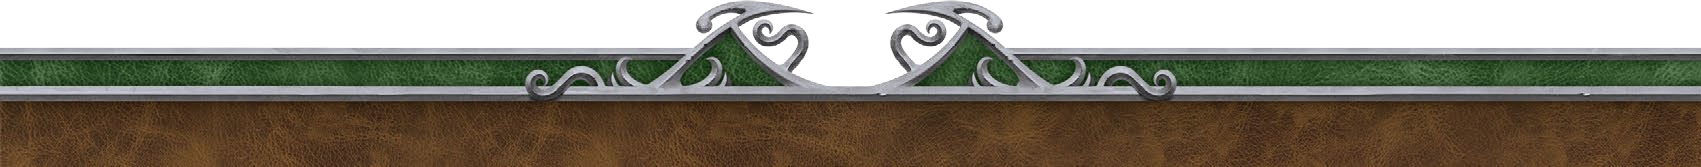
\includegraphics[width=\paperwidth,height=0.05\paperheight]{\layout/bottom.png}}}
}

\begin{document}

% !TeX spellcheck = en_US
\thispagestyle{empty}
\begin{tikzpicture}[remember picture, overlay, inner sep=10pt]
  \iftoggle{noartbackground}{}{
    \node(cover)[anchor=center] at (current page.center) {
      \includegraphics[height=\paperheight, keepaspectratio]{\layout/cover.jpg}
    };
  }
  \node(title)[minimum width = \paperwidth, anchor=center, yshift=\dimexpr-10em\relax] at (current page.north) {
    \includegraphics[width=0.6\paperwidth]{\layout/cover_title.png}
  };
  \node(subtitle)[anchor=center, yshift=12em] at (current page.south) {
    
\includegraphics[width=0.6\paperwidth]{\layout/cover_subtitle.png}
  };
\end{tikzpicture}

% Render phantom SVGs before their use in tabular env
\phantom{
  \includesvg[height=0.1px]{\svgs/bronze.svg}
  \includesvg[height=0.1px]{\svgs/bronze.svg}
  \includesvg[height=0.1px]{\svgs/silver.svg}
  \includesvg[height=0.1px]{\svgs/golden.svg}
  \includesvg[height=0.1px]{\svgs/azure.svg}
  \includesvg[height=0.1px]{\svgs/gold.svg}
  \includesvg[height=0.1px]{\svgs/building_materials.svg}
  \includesvg[height=0.1px]{\svgs/valuables.svg}
  \includesvg[height=0.1px]{\svgs/attack-yellow.svg}
  \includesvg[height=0.1px]{\svgs/defense-yellow.svg}
  \includesvg[height=0.1px]{\svgs/damage-yellow.svg}
}


\iftoggle{printable}{
  \newgeometry{
    twoside,
    top=2cm,
    bottom=3cm,
    left=2.5cm,
    right=1.5cm,
    marginparwidth=1.75cm,
    footskip=2.05cm,
  }
}{}

\author{\authortext}
\maketitle

\begin{center}
  \iftoggle{githubbuild}{
    \getenv[\githubsha]{GITHUB_SHA}
    \versionwarning{} \href{\repourl}{\StrLeft{\githubsha}{7}}.
  }{
    \versionlabel{} \input{.version}
  }

  \bigbreak

  \intro{}

  \bigbreak

  
\includegraphics[width=0.4\linewidth]{\qr/github.png} \\
  \qrgithub
\end{center}

\AddToHookNext{shipout/background}{
  \put (0in,-\paperheight){\includegraphics[width=\paperwidth,height=\paperheight]{\layout/tausta.png}}
}
\thispagestyle{empty}
\begin{tikzpicture}[remember picture, overlay]
  \node(cover)[anchor=center, yshift=9em] at (current page.south) {
    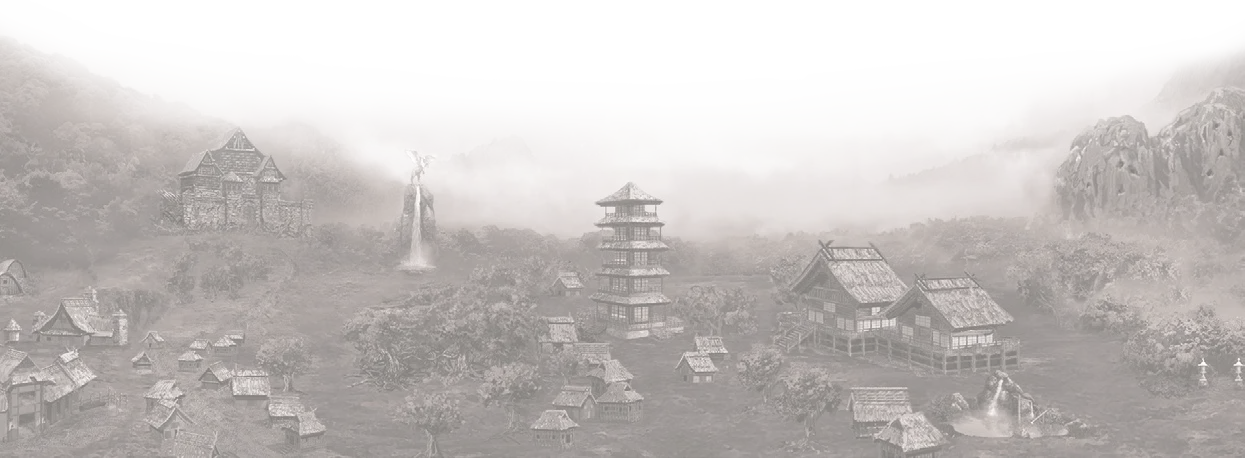
\includegraphics[width=1.01\paperwidth, keepaspectratio]{\layout/rampart_background.png}
  };
\end{tikzpicture}

\clearpage

\begin{multicols*}{2}
\tableofcontents
\vspace*{\fill}
\columnbreak
\vspace{-3em}
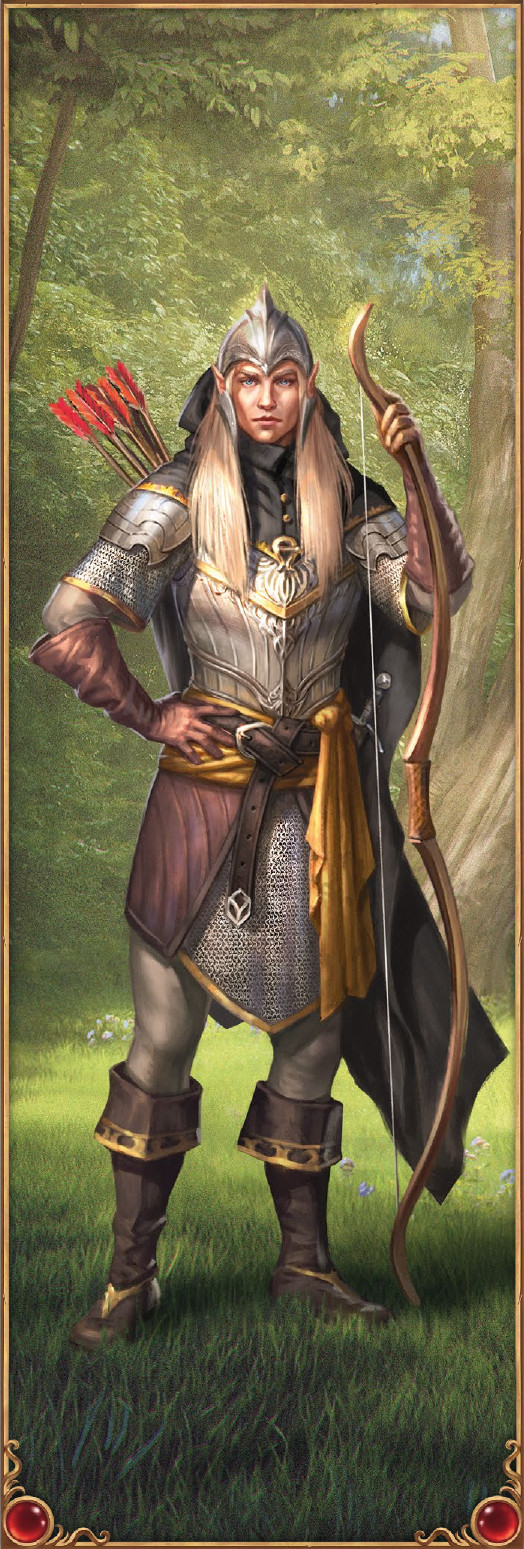
\includegraphics[width=\linewidth]{\art/elf.jpg}
\end{multicols*}

\clearpage

% !TeX spellcheck = en_US
\addsection{What to Play}{\images/forgetfulness.png}

\begin{multicols}{2}

Follow these suggestions if you're not sure which scenario is best for you.

\subsection*{Cooperative Mode}

If you're new to the game and want to try \textbf{learning the rules}, start with \pagelink{Emerald Island}{Emerald Island}.
For a big adventure for \textbf{up to 6 players} with an epic battle at the end, try \pagelink{Titans' Stronghold}{Titans' Stronghold}.
For more tactical play for two players, try \pagelink{Sentinels}{Sentinels}.

\subsection*{Clash Mode}

If you'd like to play a 2- or 4-player ``capture the Grail'' scenario with interesting twists, try \pagelink{Bloody Grail}{Bloody Grail}.
For an exciting boss fight for 3 players, choose \pagelink{The Hunt}{The Hunt}.
For an inevitable epic battle between two players with a possible siege, play \pagelink{Dragoncurse Castle}{Dragoncurse Castle}.

\subsection*{Campaign}

There is a 3-scenario Inferno \pagelink{1. A Devilish Plan}{Dungeons and Devils} Campaign at the end if you prefer solo play.

\subsection*{Recommendations}

For information regarding your play time, strategizing, and custom rules, checkout out \pagelink{Recommendations}{recommendations} at the and of this book.

\end{multicols}

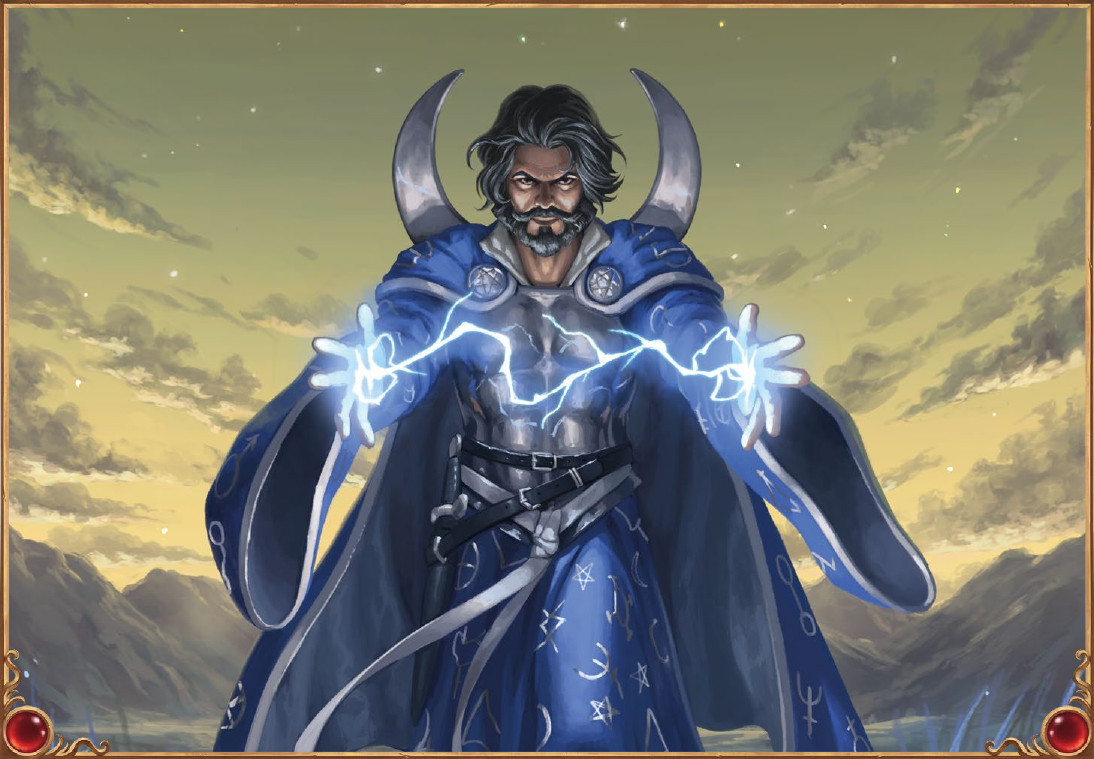
\includegraphics[width=\linewidth]{\art/enchanter.jpg}


\addscenariogroup{Cooperative Scenarios}{\layout/coops.png}

\clearpage

% !TeX spellcheck = en_US
\addscenariosection{1}{Cooperative scenario}{Sentinels}{\images/sentinel.png}

\begin{multicols}{2}

\textbf{Author:} silence70011

\textbf{Source:} \href{https://discord.com/channels/740870068178649108/1233112440322002964/1233112440322002964}{Archon Studio Discord}

\textit{There is a world beyond ours, filled with beasts and monsters, barely contained by a formation of four sacred Obelisks.
  But the power of these stones is waning, and a breach is imminent.
  When it happens, only you and your ally will stand between the hordes and the total devastation of these lands.
}

\subsection*{\MakeUppercase{Scenario Length}}

This scenario is played over 12 rounds.

\subsection*{\MakeUppercase{Player Setup}}

\textbf{Player Count:} 2

\textbf{Starting Resources:}\par
\resources{10}{2}{1}

\textbf{Starting Income:}\par
\resources{10}{2}{1}

\textbf{Starting Units:}
\begin{itemize}
  \item A Pack of \svg{bronze} units with the \textit{lowest} recruitment cost.
  \item A Few \svg{bronze} units with the \textit{highest} recruitment cost.
\end{itemize}

\textbf{Town Buildings:} \svg{bronze} Dwelling, Citadel

\textbf{Map tile Pool:} Each player takes 1 random Near (IV--V) Map tile and 1 random Far (II--III) Map tile. These tiles should not contain any Obelisks.

\textbf{Additional Bonus:} Search (2) the Artifact Deck

\subsection*{\MakeUppercase{Map Setup}}

Take the following Map tiles and arrange them as shown in the scenario map layout:

\textbf{2 × Starting (I) Map tile}
\begin{itemize}
  \item Starting Tiles of your chosen factions.
  \item Ignore their yellow borders.
\end{itemize}

\textbf{4 × Far (II--III) Map tile}

\textbf{4 × Near (IV--V) Map tile}
\begin{itemize}
  \item All Near Map tiles must have Obelisks.
\end{itemize}

\subsection*{\MakeUppercase{Victory Conditions}}

Defeat all invading armies.

\subsection*{\MakeUppercase{Defeat Conditions}}

An undefeated enemy army remains at the end of Round 12.

One of your towns is captured, or a main hero is defeated in a battle (retreat doesn't count).

\subsection*{\MakeUppercase{Timed Events}}

\textbf{\nth{6} Round:}
\begin{itemize}
  \item Remove all Black cubes from every Windmill, Water Wheel, and Mystical Garden on the map.
  \item Spawn an enemy army following the rules outlined below.
\end{itemize}

\textbf{\nth{7} and \nth{8} Rounds:}
\begin{itemize}
  \item Spawn an enemy army following the rules outlined below.
\end{itemize}

\textbf{\nth{9} Round:}
\begin{itemize}
  \item Repeat the Timed Events of Round 6.
\end{itemize}

\textbf{\nth{10} Round:}
\begin{itemize}
  \item Repeat the Timed Events of Rounds \mbox{7 and 8.}
\end{itemize}
\vspace{-0.5em}

\subsection*{\MakeUppercase{Additional Rules}}

\begin{itemize}
  \item Players can trade resources when one of the active player's heroes visits a trading post or stands on a field adjacent to an allied hero.
  \item The hero who defeats an enemy army gains 2 \svg{experience}.
    The victorious player rolls two Treasure Dice and resolves one of them.
  \item Additionally, no player can:
  \begin{itemize}
      \item Attack other Heroes.
      \item Capture a Mine or Settlement that is already Flagged.
  \end{itemize}
\end{itemize}

\subsection*{\MakeUppercase{Enemy Spawning\\and Movement}}

\begin{itemize}
  \item Enemy armies spawn on a random Obelisk field (use hero miniatures from factions not in play).
  \item Determine which Obelisk field by rolling 2 Attack Dice. Apply the results as follows (D1/D2), reroll any 0:
  \begin{itemize}[leftmargin=15pt]
    \item $+1$/$+1$ = North, $+1$/$-1$ = East
    \item $-1$/$+1$ = West, $-1$/$-1$ = South
  \end{itemize}
  \item For a more balanced distribution, in Rounds 7 and 9, only roll the second Attack Die (D2). For D1, take the opposite result from what was rolled in the previous Round.
  Rounds 8 and 10 are entirely random.
  \item If the tile where an enemy is to spawn hasn't been discovered yet, flip it over and orient it as preferred.
  \item If there is a hero on the field where the enemy spawns, a fight starts immediately.
  \item Enemy armies move at the end of every turn, starting with the turn they spawned.
  \item Enemy armies have 3 MPs per round.
  \item Enemy armies move as described in the rulebook (p.\,33), but instead of capturing, they destroy everything in their path.
    Place Black cubes on any field they pass through, treating those fields as empty from that point on.
  \item If an enemy's movement could go in different directions, the players decide which way they go.
\end{itemize}

\subsection*{\MakeUppercase{Combat with\\Enemy Armies}}

\begin{itemize}
  \item Fighting enemy armies over more than one Combat Round does not cost Movement Points.
  \item During a battle with an enemy army, a hero can retreat whenever a friendly unit is about to activate.
    A retreating main Hero loses all remaining MPs and is returned to an allied town or settlement of their choice, keeping all remaining units.
  \item Retreating secondary heroes are removed from the game, but their remaining units are kept.
  \item Killed enemy units do not respawn.
\end{itemize}

\subsection*{\MakeUppercase{Boss Army}}

\begin{itemize}
  \item In Round 10, a Boss Army spawns. It is different from previous armies because it is reinforced from a fixed pool of neutral units (reinforcement pool = number in brackets in the table below).
  \item At the beginning of the \nth{2} combat round and every following round, 2 units reinforce the remaining army from the shuffled reinforcement pool (up to a maximum of 5 units) to continue the fight until either the player retreats or every neutral unit from the reinforcement pool is killed. \textit{If the number of enemy units at the beginning of a round is 1 or lower, draw up to a total of 4 units (i.e., there are always 4 or 5 enemy units on the board after reinforcing, if available).}
  \item Place the reinforcing units on the enemy base line, starting from the left with the lowest initiative (\svg{unit_ranged} units first). If necessary, continue on the next line in the same order.
  \item When a player retreats, the enemy army draws up to the ``minimum'' of 4 units and takes these as starting units to the next fight.
\end{itemize}

\columnbreak

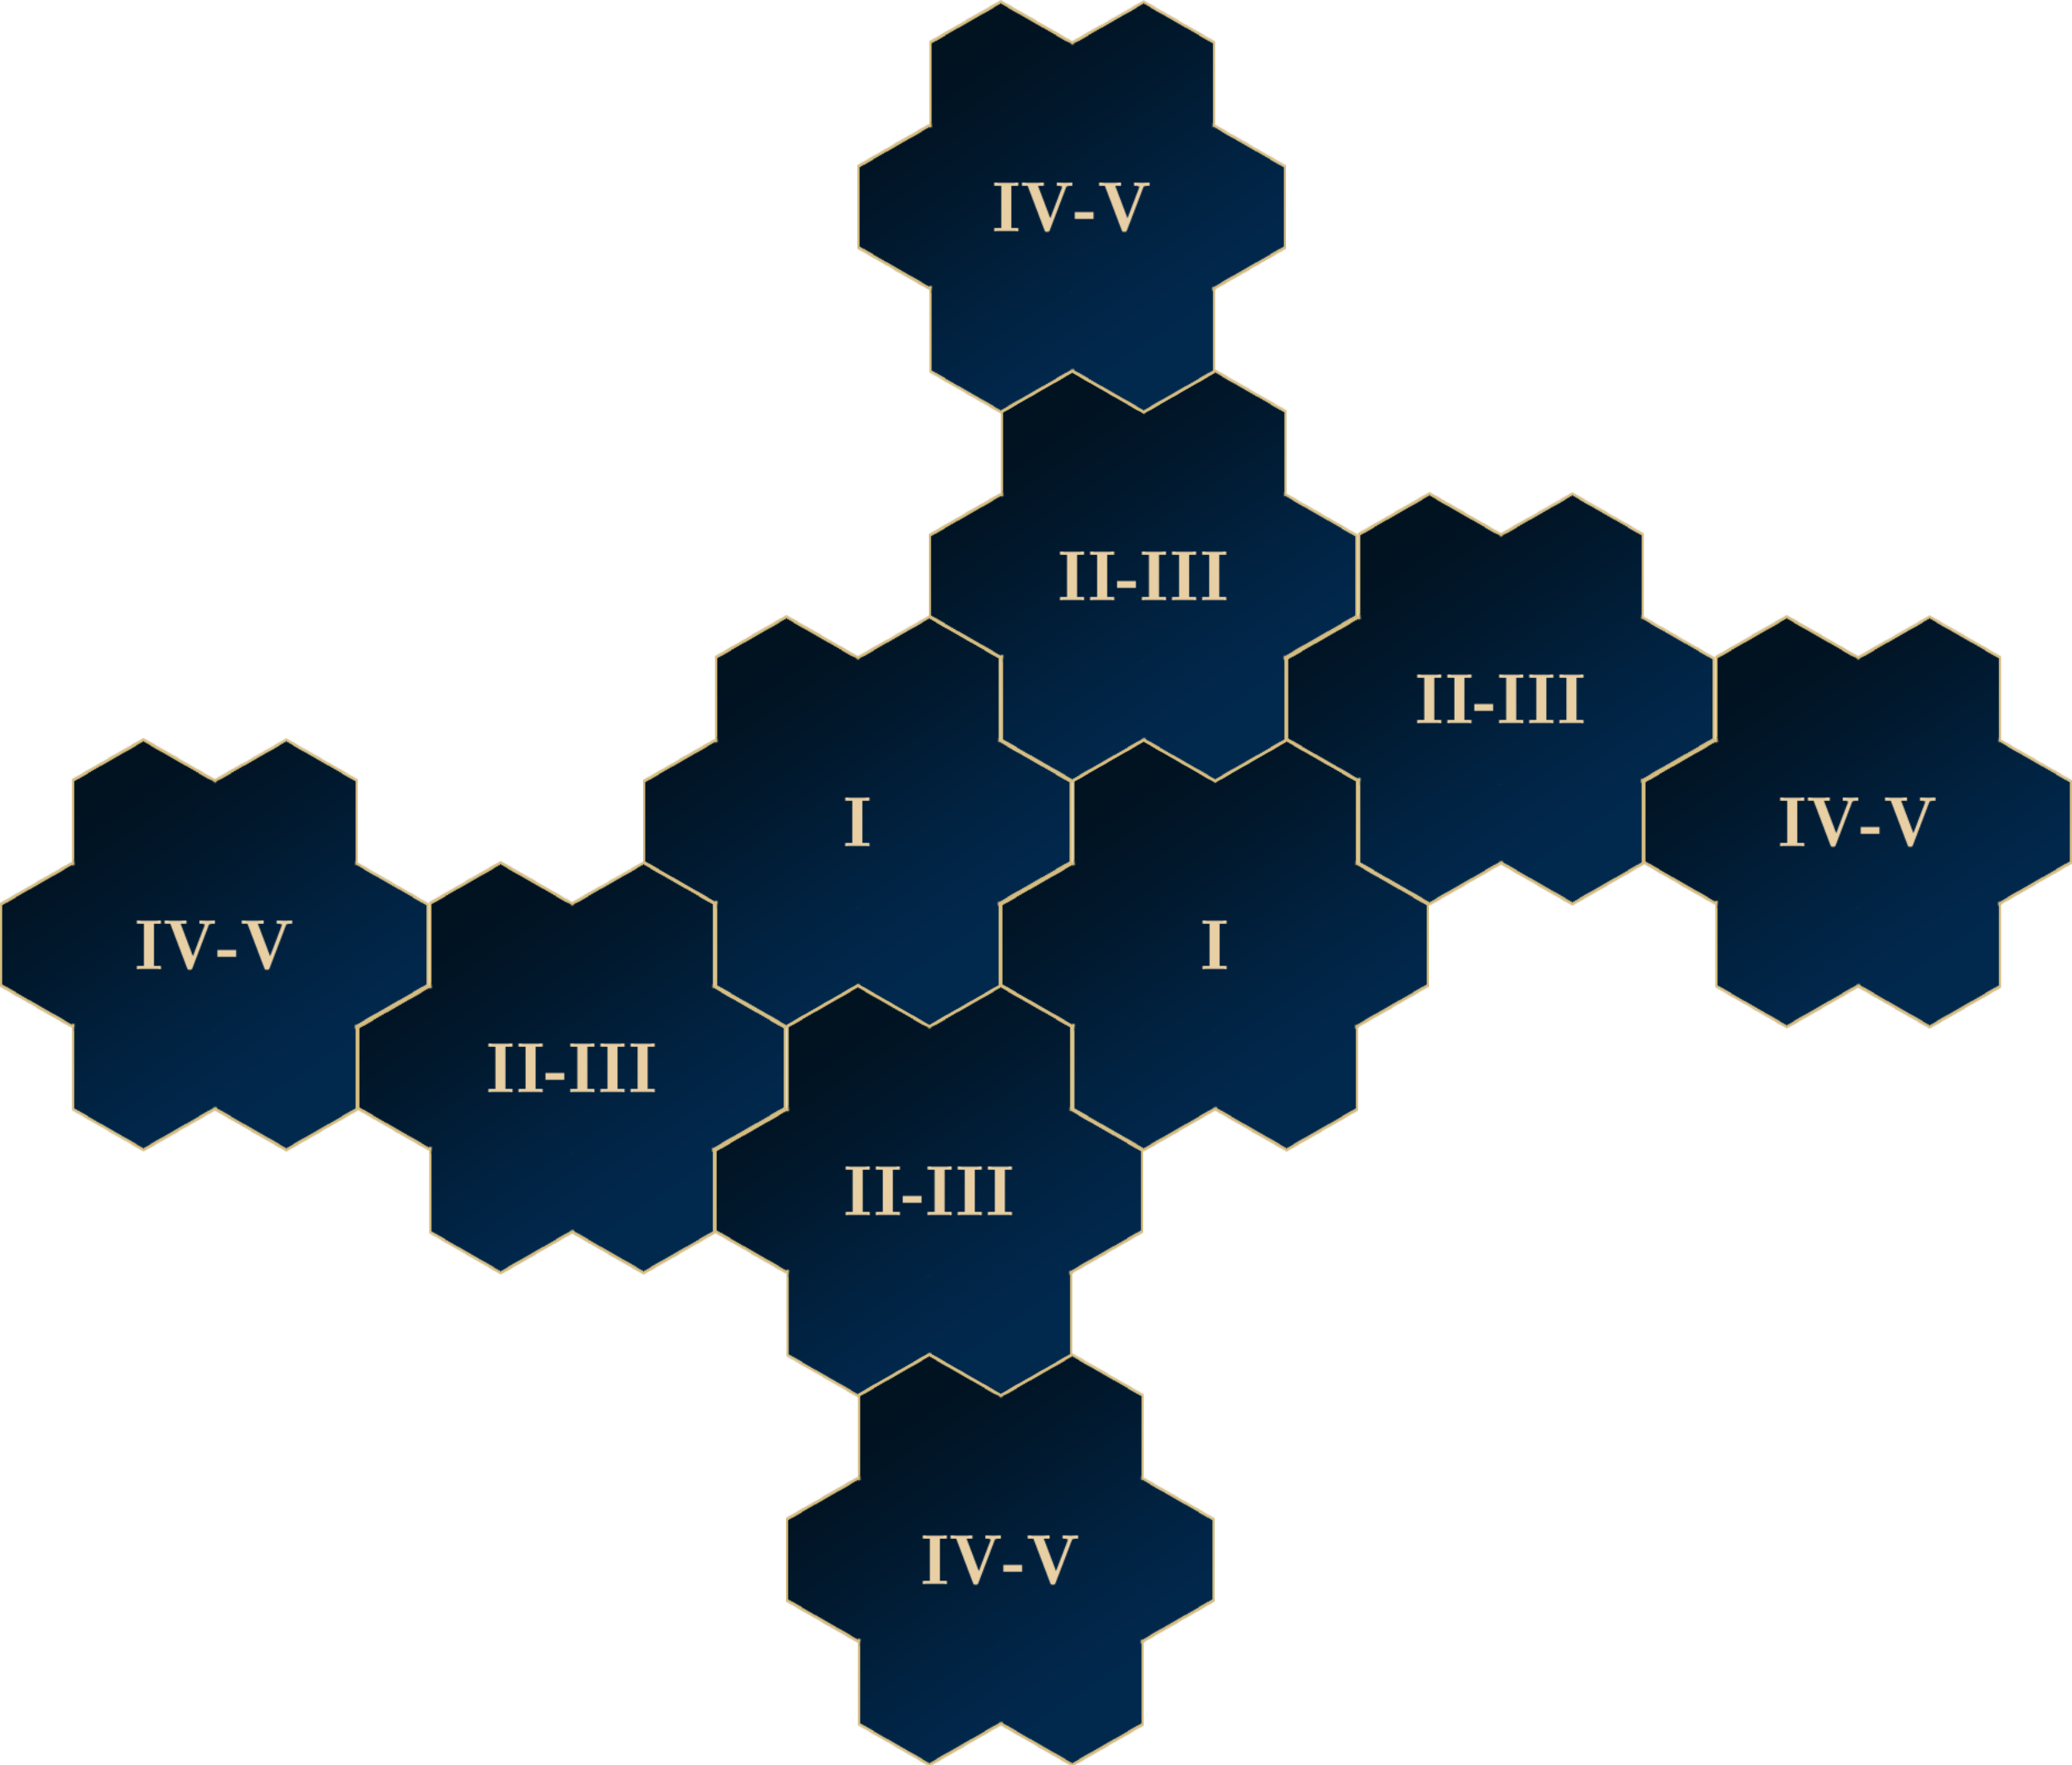
\includegraphics[width=0.4\paperwidth]{\_assets/maps/sentinels.png}

\end{multicols}

\vspace*{\fill}

\hommtable[]{20}{
  \centering
  \medskip
  \textbf{Strength of Enemy Armies}\\
  \bigskip

  \newcommand{\bronze}[0]{\svg[12]{bronze}}
  \newcommand{\silver}[0]{\svg[12]{silver}}
  \newcommand{\golden}[0]{\svg[12]{golden}}
  \newcommand{\azure}[0]{\svg[12]{azure}}

  \begin{tabularx}{\linewidth}{p{0.15\linewidth}XXXX} & \darkcell{Rounds 6 + 7} & \darkcell{Rounds 8 + 9} & \darkcell{Round 10}\\
  \darkcell[1.4]{Easy}
    & \lightcell[1.4]{\bronze \silver \silver \silver \golden}
    & \lightcell[1.4]{\silver \silver \silver \golden \golden}
    & \lightcell[1.4]{\silver \silver \golden \azure \footref{azure} \linebreak
      (2\bronze, 4\silver, 3\golden, 1\azure)}\\
  \darkcell[1.4]{Normal}
    & \lightcell[1.4]{\silver \silver \silver \golden \golden}
    & \lightcell[1.4]{\silver \silver \silver \golden \azure}
    & \lightcell[1.4]{\golden \golden \golden \azure \footref{azure} \linebreak
      (2\silver, 7\golden, 1\azure)}\\
  \darkcell[1.4]{Hard}
    & \lightcell[1.4]{\silver \silver \golden \golden \golden}
    & \lightcell[1.4]{\silver \silver \golden \golden \azure}
    & \lightcell[1.4]{\golden \golden \azure \azure \footref{azure} \linebreak
      (2\silver, 6\golden, 2\azure)}\\
  \darkcell[1.4]{Impossible}
    & \lightcell[1.4]{\silver \golden \golden \golden \golden}
    & \lightcell[1.4]{\golden \golden \golden \golden \azure}
    & \lightcell[1.4]{\golden \azure \azure \azure \footref{azure} \linebreak
      (7\golden, 3\azure)}\\
  \end{tabularx}
}

\vspace*{\fill}

\footnotetext[1]{Always 1 unit of Azure Dragons (starting units of Boss Army). The rest is random\label{azure}.}


\clearpage

% !TeX spellcheck = en_US
\addscenariosection{1}{Cooperative scenario}{Titans' Stronghold}{\images/earthquake.png}

\begin{multicols*}{2}

\textbf{Author:} Invoceusse

\textbf{Source:} \href{https://discord.com/channels/740870068178649108/1219333721019256943}{Archon Studio Discord}

\textit{A long time ago, a mighty fortress was built to house the fantastic and murderous Titans.
  No one has ever entered and returned to tell the tale.
  Now, there are rumors about the death of the guardians and an incredible amount of treasures, potentially including the best bow in the world.\\
  If this legend of the empty fort is true, it's time for excavation.\\
  But for now, you and your allies need to find the keys spread across Antagarich to open the gate of the Titans' Stronghold.
}
\subsection*{\MakeUppercase{Scenario Length}}

This scenario is played over 16 rounds (15 on Impossible difficulty).

\subsection*{\MakeUppercase{Player setup}}

\textbf{Player Count:} 1 -- 6

\textbf{Starting Resources:}\par
\resources{30}{8}{2}

\textbf{Starting Income:}\par
\resources{10}{2}{1}

\textbf{Starting Units:}
\begin{itemize}
  \item A Pack of \svgunit{bronze} units of your choice
  \item A Few \svgunit{bronze} units of your choice
\end{itemize}

\textbf{Town Buildings:} None

\textbf{Map tile Pool:} None

\textbf{Additional Bonus:} None

\subsection*{\MakeUppercase{Map Setup}}

Take the following Map tiles and arrange them as shown in the scenario map layout ($P$ stands for the number of players):

$\boldsymbol{P}$ \textbf{× Starting (I) Map tile}
\begin{itemize}
  \item Starting Tiles of your chosen factions.
  \item Ignore their yellow borders.
\end{itemize}

$\boldsymbol{2 P}$ \textbf{× Far (II--III) Map tile}

$\boldsymbol{2 P}$ \textbf{× Near (IV--V) Map tile}

$\boldsymbol{(P + 1)}$ \textbf{× Center (VI--VII) Map tile}

If you don't have enough VI--VII tiles, you can use another tile near to tile I.
The center of this tile is the Titans' Stronghold.

\subsection*{\MakeUppercase{Victory Conditions}}

Kill all units in the Titans' Stronghold (the center of tile VI--VII next to tiles I).

\subsection*{\MakeUppercase{Defeat Conditions}}

There are undefeated units left in the Titans' Stronghold at the end of Round 16 (15 on Impossible difficulty).

\subsection*{\MakeUppercase{Timed Events}}

\textbf{\nth{4}, \nth{8} and \nth{12} Rounds:}
\begin{itemize}
  \item Remove all Black cubes from every Windmill, Water Wheel, and Mystical Garden on the map.
\end{itemize}

\vspace*{\fill}\columnbreak

\subsection*{\MakeUppercase{Additional Rules}}
\begin{itemize}
  \item Remember: the center of VI--VII tile next to all I tiles is the Titans' Stronghold.
  \item No one can enter the Titans' Stronghold until all other VII fields are flagged by any player.
  \item After defeating a level VII neutral army, instead of resolving the field, the player chooses an option three times from the following list (an option may be chosen multiple times):
    \begin{itemize}[leftmargin=12pt]
      \item Another player (your choice) gains 5 \svg{gold}
      \item Another player (your choice) gains 2 \svg{building_materials}
      \item Another player (your choice) gains 1 \svg{valuables}
    \end{itemize}
  Then, flag the VII field with a faction cube.
  (There is no bonus in solo play!)
  \item Ignore all yellow borders in I tiles.
  \item You can use your build token to give your resources to another player.
  \item Two players can use their build tokens to exchange artifacts and/or spells.
  \item Whenever a player visits an Obelisk, that player rolls one treasure die and one resource die, and resolves one of them.
  \item When all VII fields (excluding the Titans' Stronghold) are flagged, randomly draw and shuffle the specified number (see the next page) of Neutral Unit cards from each of their corresponding decks to create a separate deck of Neutral Units for the Titans' Stronghold (the deck of the Titans' Stronghold is sometimes split in two because certain scenarios are otherwise impossible to implement with the cards from certain expansions).
  \item Any time a Hero enters the Titans' Stronghold, they draw 5 cards from the Titans' Stronghold deck instead of from the Neutral Unit card decks. The units are placed on the Combat board (see page 29, ``Neutral Unit Setup'' in the Core Rulebook). Players attempt to defeat the units they find in the Titans' Stronghold. Any Neutral Units defeated during combat in the Titans' Stronghold are returned to their respective Neutral Unit decks instead of the Titans' Stronghold deck. Any Neutral Units surviving combat in the Titans' Stronghold are shuffled back into the Titans' Stronghold deck. If there are not enough Unit cards in this deck, draw as many Unit cards as are available and place them on the Combat board.
  \item Combat in the Titans' Stronghold now costs 1 MP to extend per Combat round, just like Combat against non-Azure tier units.
  \item Additionally, no player can:
  \begin{itemize}
    \item Attack other Heroes.
    \item Capture a Mine or Settlement that is already controlled.
  \end{itemize}
\end{itemize}

\vspace*{\fill}

\begin{center}
  
\includegraphics[width=\linewidth]{\art/dimension_door.png}
\end{center}

\vspace*{\fill}

\end{multicols*}

\newpage

\hommtable[]{28}{
  \centering
  \medskip
  \textbf{Strength of Titans' Stronghold Armies}\\
  \bigskip

  \newcommand{\bronze}[0]{\svg[12]{bronze}}
  \newcommand{\silver}[0]{\svg[12]{silver}}
  \newcommand{\golden}[0]{\svg[12]{golden}}
  \newcommand{\azure}[0]{\svg[12]{azure}}

  \begin{tabularx}{\linewidth}{p{0.15\linewidth}XXXX} & \darkcell{Easy} & \darkcell{Normal} & \darkcell{Hard} & \darkcell{Impossible}\\
  \darkcell[1.2]{1 player}
    & \lightcell[1.2]{3\bronze 2\silver 1\golden 1\azure}
    & \lightcell[1.2]{2\bronze 2\silver 2\golden 1\azure}
    & \lightcell[1.2]{2\bronze 2\silver 2\golden 2\azure}
    & \lightcell[1.2]{1\bronze 2\silver 2\golden 3\azure}\\
  \darkcell[1.2]{2 players}
    & \lightcell[1.2]{5\bronze 5\silver 3\golden 1\azure}
    & \lightcell[1.2]{4\bronze 5\silver 3\golden 2\azure}
    & \lightcell[1.2]{2\bronze 5\silver 5\golden 3\azure}
    & \lightcell[1.2]{1\bronze 5\silver 7\golden 4\azure}\\
  \darkcell[1.8]{3 players}
    & \lightcell[1.8]{8\bronze 7\silver 4\golden 2\azure}
    & \lightcell[1.8]{6\bronze 7\silver 5\golden 3\azure}
    & \lightcell[1.8]{2\bronze 3\silver 4\golden 3\azure \linebreak
      Then\linebreak
      2\bronze 4\silver 3\golden 2\azure}
    & \lightcell[1.8]{1\bronze 3\silver 5\golden 3\azure \linebreak
      Then\linebreak
      1\bronze 4\silver 5\golden 3\azure}\\
  \darkcell[1.8]{4 players}
    & \lightcell[1.8]{10\bronze 10\silver 6\golden 2\azure}
    & \lightcell[1.8]{8\bronze 10\silver 6\golden 4\azure}
    & \lightcell[1.8]{2\bronze 5\silver 5\golden 3\azure \linebreak
      Then\linebreak
      2\bronze 5\silver 5\golden 3\azure}
    & \lightcell[1.8]{1\bronze 5\silver 7\golden 4\azure \linebreak
      Then\linebreak
      1\bronze 5\silver 7\golden 4\azure}\\
  \darkcell[1.8]{5 players}
    & \lightcell[1.8]{6\bronze 6\silver 4\golden 1\azure \linebreak
      Then\linebreak
      7\bronze 6\silver 3\golden 2\azure}
    & \lightcell[1.8]{5\bronze 6\silver 4\golden 2\azure \linebreak
      Then\linebreak
      5\bronze 6\silver 4\golden 3\azure}
    & \lightcell[1.8]{3\bronze 6\silver 6\golden 4\azure \linebreak
      Then\linebreak
      3\bronze 6\silver 6\golden 4\azure}
    & \lightcell[1.8]{1\bronze 6\silver 8\golden 6\azure \linebreak
      Then\linebreak
      2\bronze 6\silver 8\golden 5\azure}\\
  \darkcell[1.7]{6 players}
    & \lightcell[1.8]{8\bronze 8\silver 4\golden 1\azure \linebreak
      Then\linebreak
      7\bronze 7\silver 5\golden 2\azure}
    & \lightcell[1.8]{6\bronze 8\silver 4\golden 3\azure \linebreak
      Then\linebreak
      6\bronze 7\silver 5\golden 3\azure}
    & \lightcell[1.8]{3\bronze 8\silver 7\golden 5\azure \linebreak
      Then\linebreak
    3\bronze 7\silver 8\golden 4\azure}
    & \lightcell[1.8]{3\bronze 7\silver 11\golden 6\azure \linebreak
    Then\linebreak
    3\bronze 8\silver 10\golden 6\azure}\\
  \end{tabularx}
}

\vspace*{\fill}

\begin{center}
  \transparent{0.3}{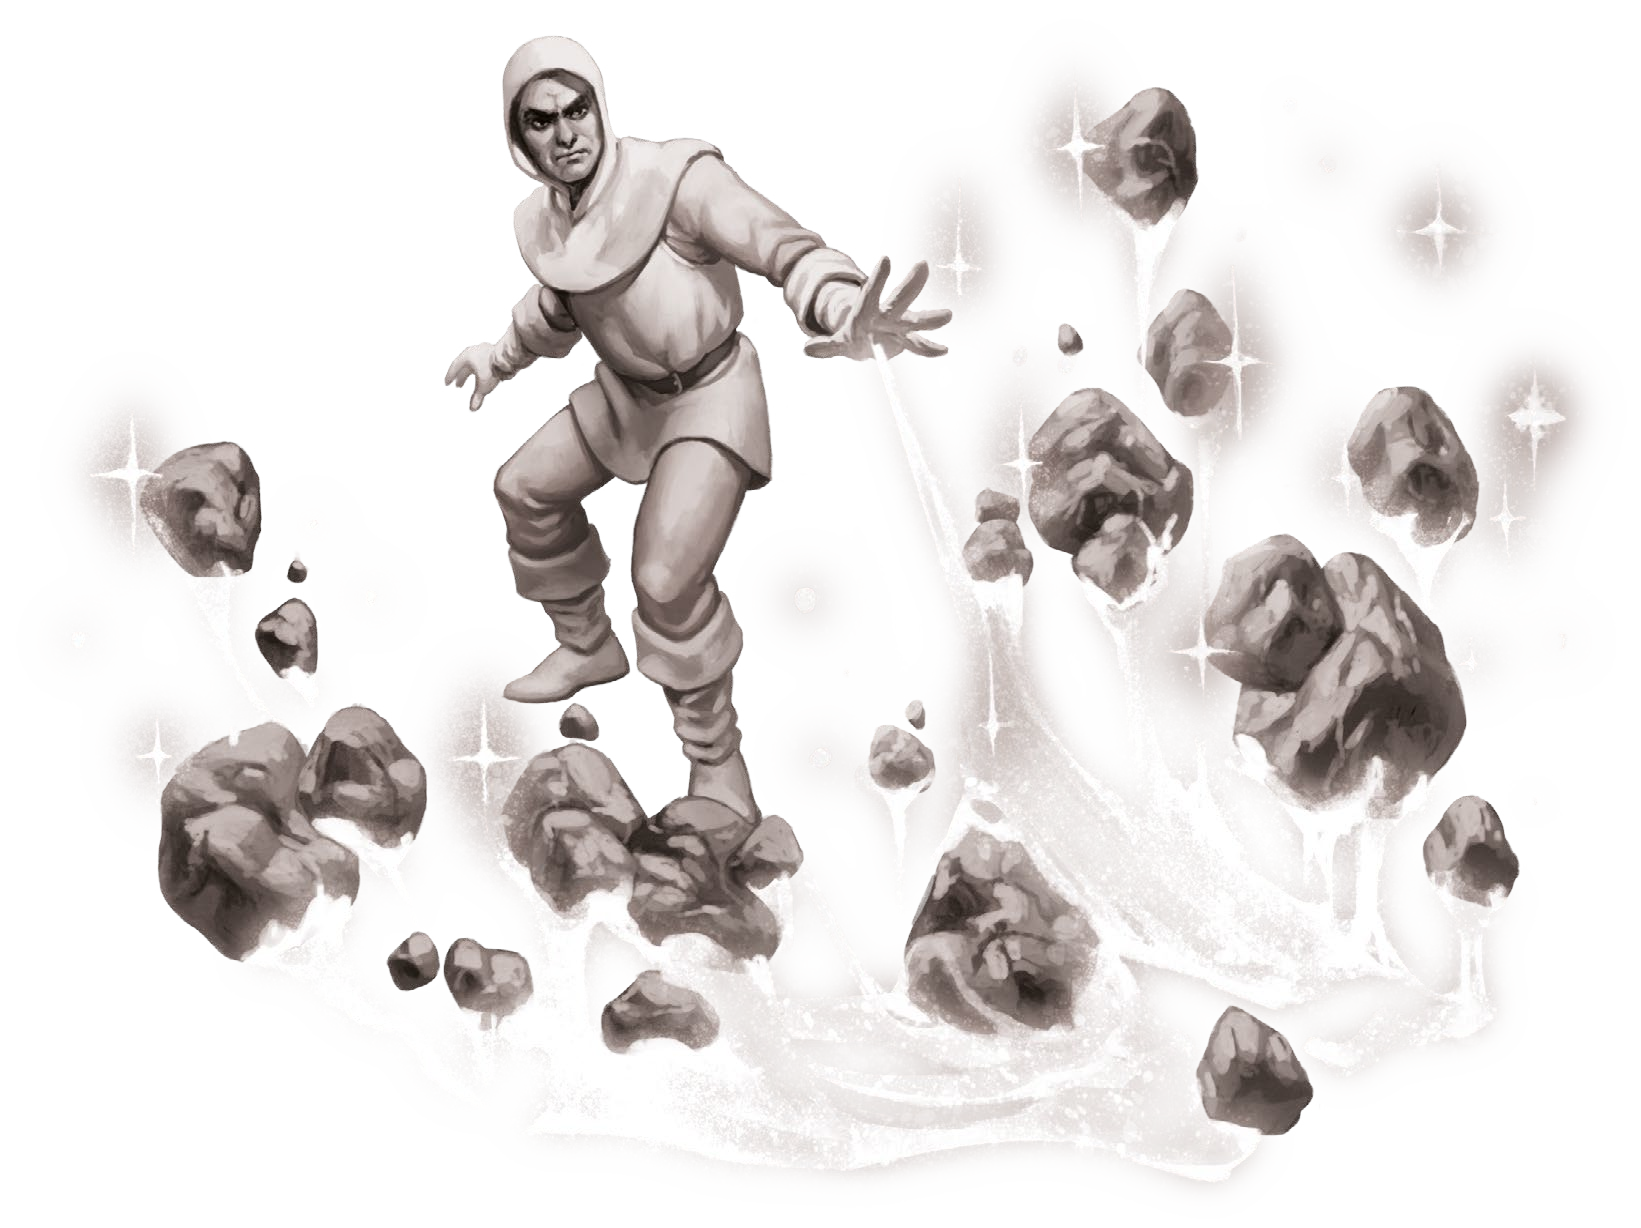
\includegraphics[width=0.6\linewidth, keepaspectratio]{\art/land_mine.png}}
\end{center}

\vspace*{\fill}

\newpage

\begin{minipage}{0.4\paperwidth}
  \centering
  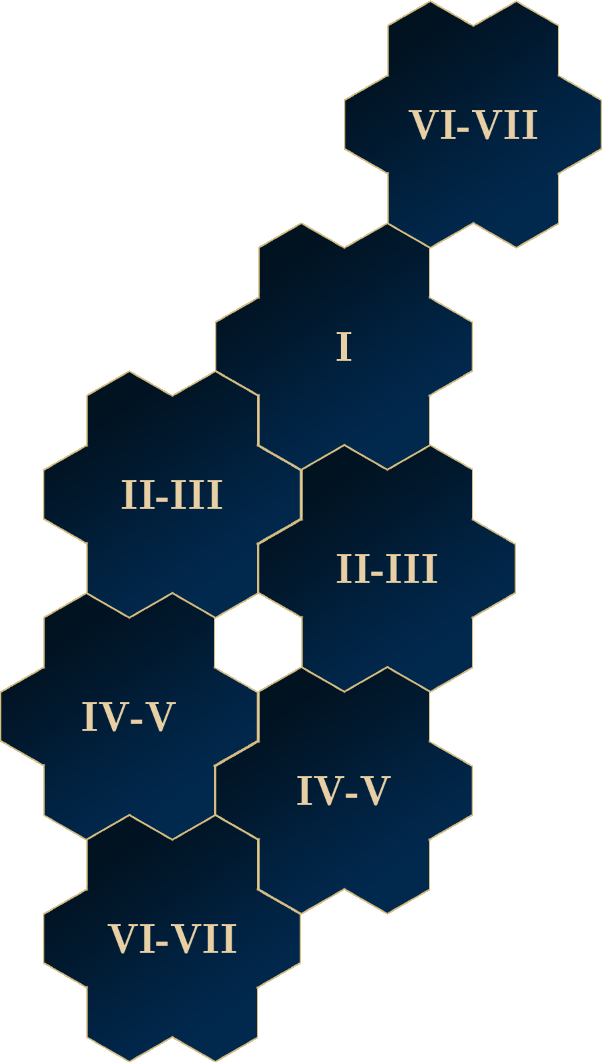
\includegraphics[width=0.18\paperwidth]{\_assets/maps/titans-1.png}
  \captionof{figure}{1-PLAYER SCENARIO}
\end{minipage}
\begin{minipage}{0.4\paperwidth}
  \centering
  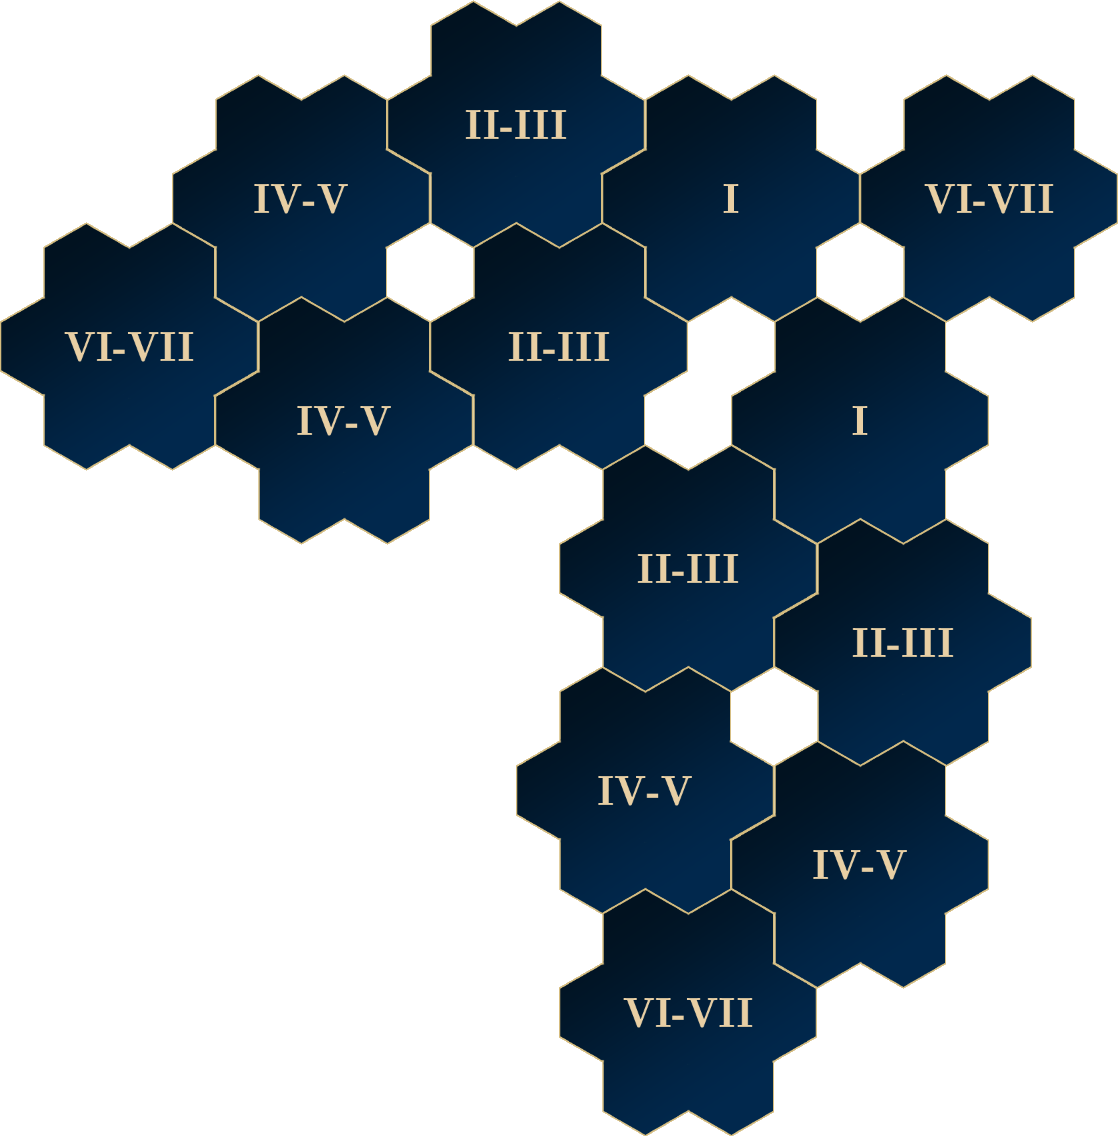
\includegraphics[width=0.36\paperwidth]{\_assets/maps/titans-2.png}
  \captionof{figure}{2-PLAYER SCENARIO}
\end{minipage}
\vspace{1em}
\linebreak
\begin{minipage}{0.4\paperwidth}
  \centering
  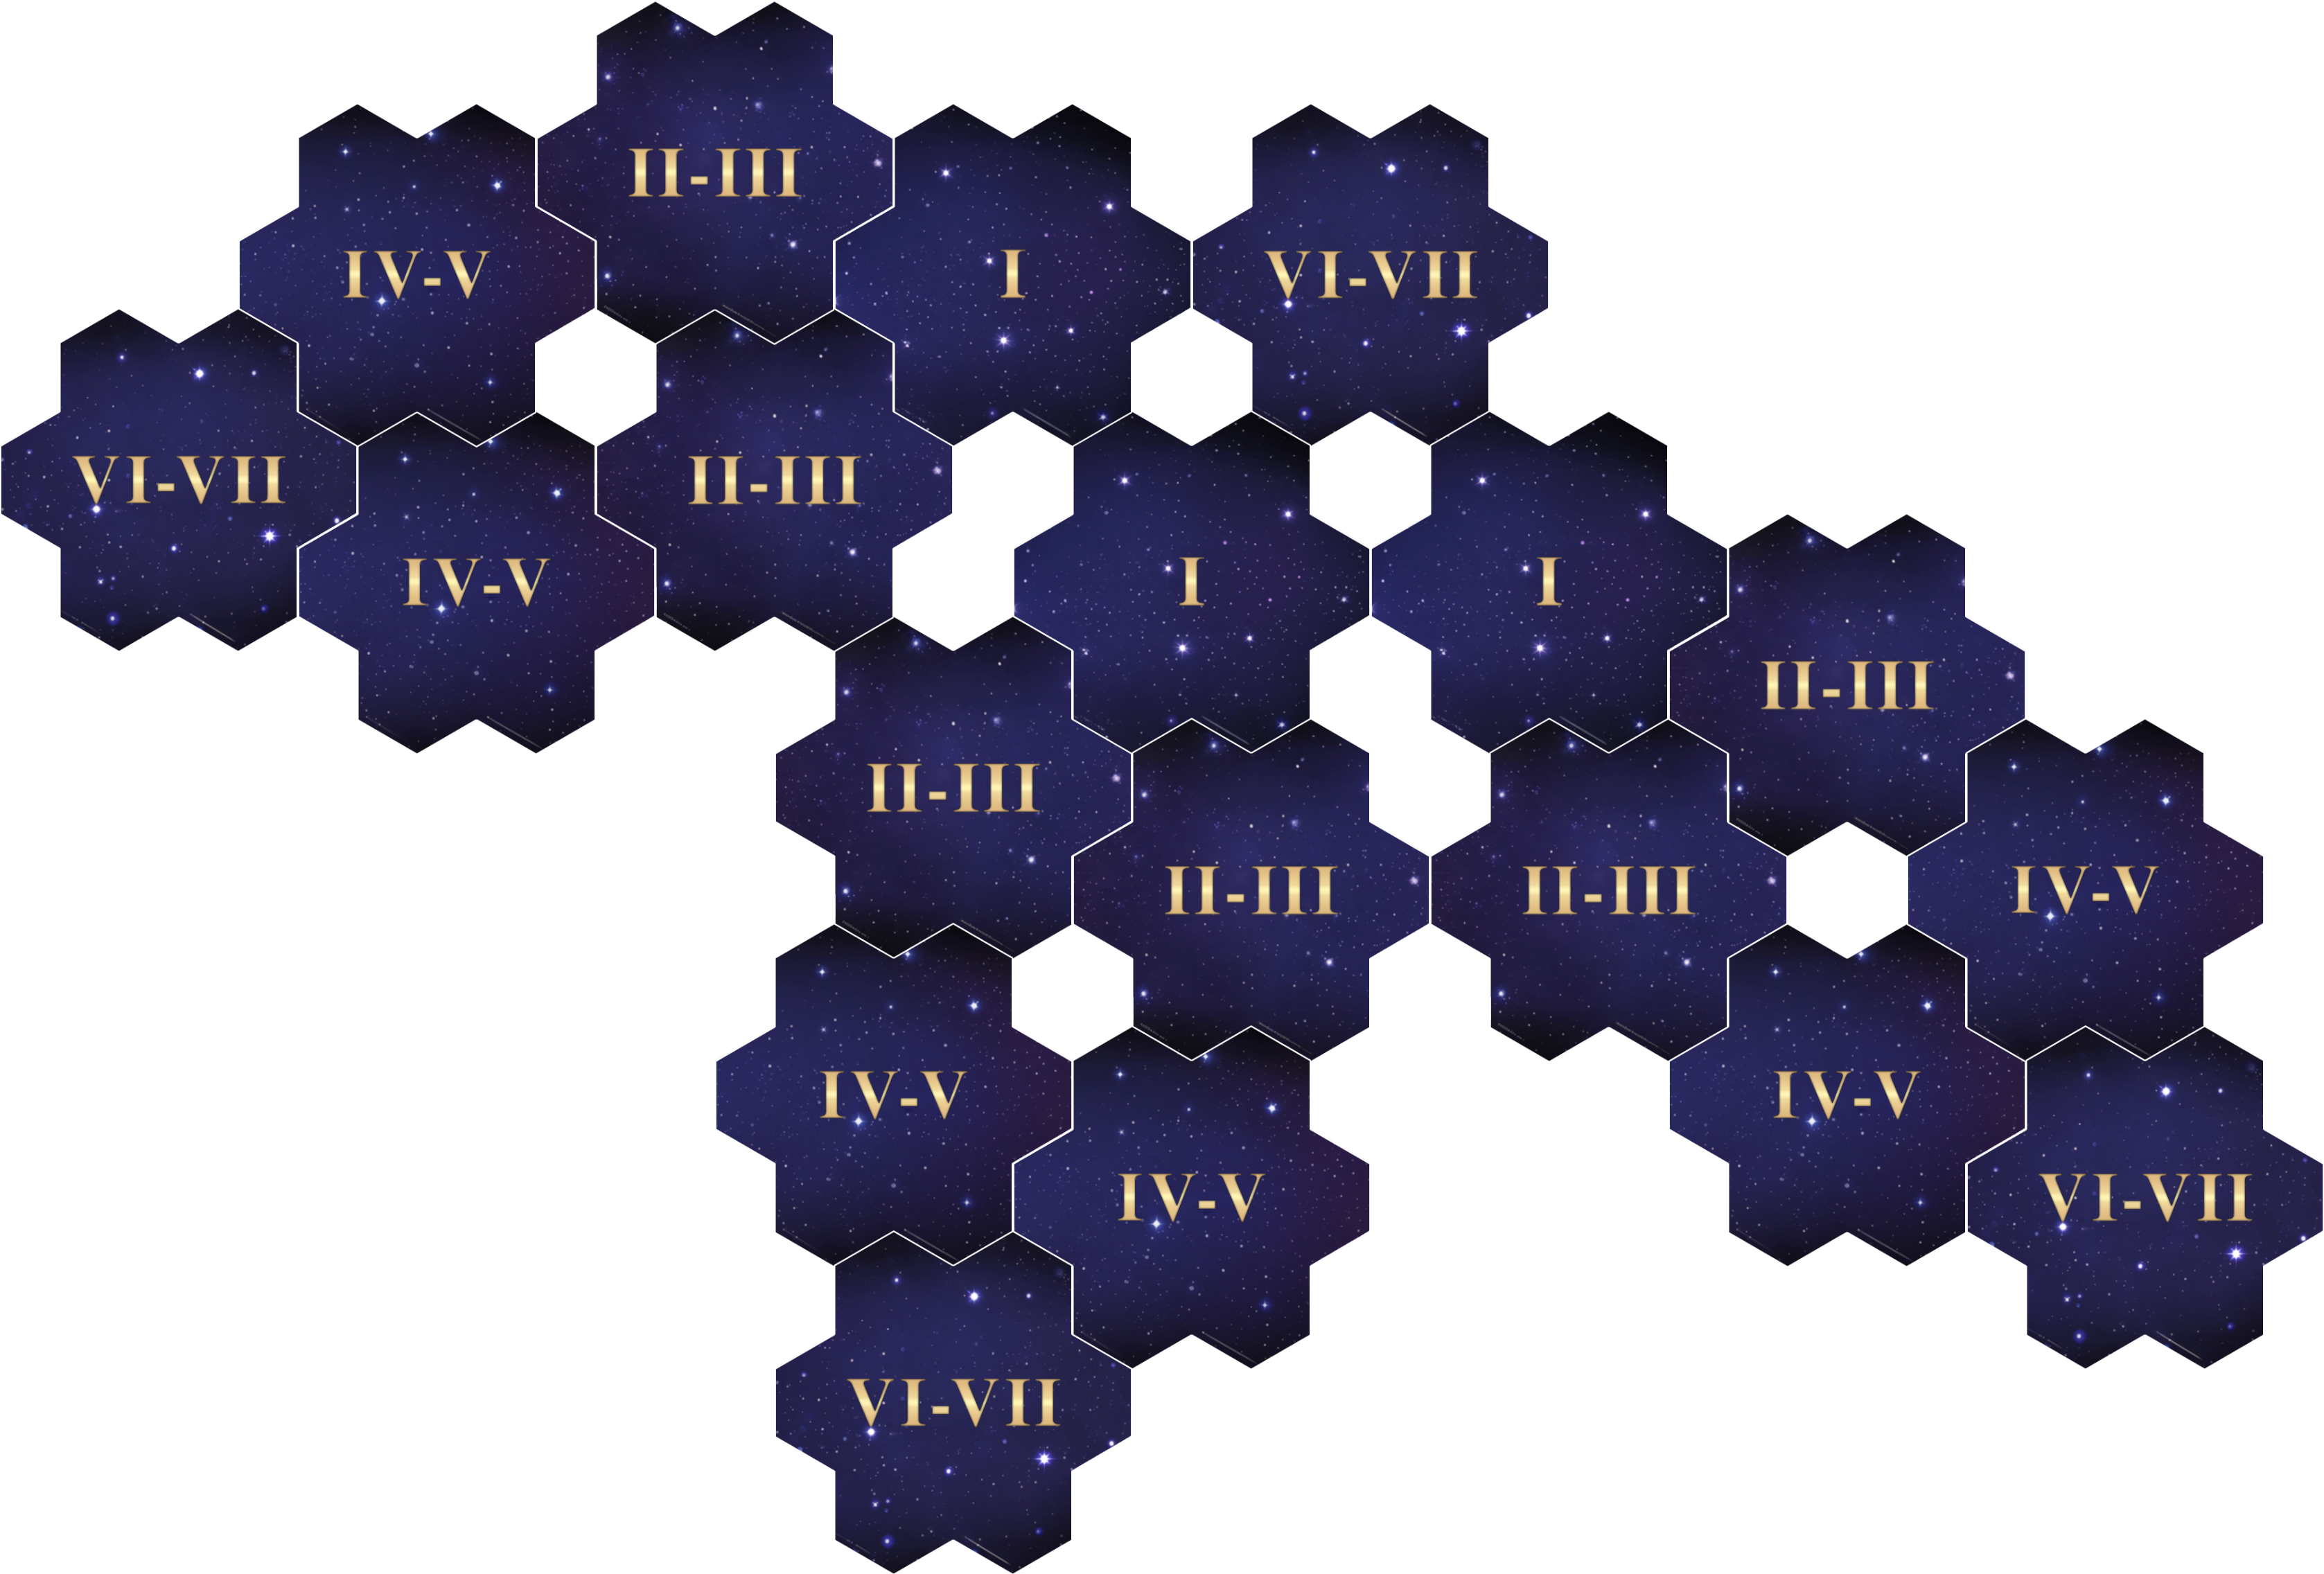
\includegraphics[width=0.38\paperwidth]{\_assets/maps/titans-3.png}
  \captionof{figure}{3-PLAYER SCENARIO}
\end{minipage}
\begin{minipage}{0.4\paperwidth}
  \centering
  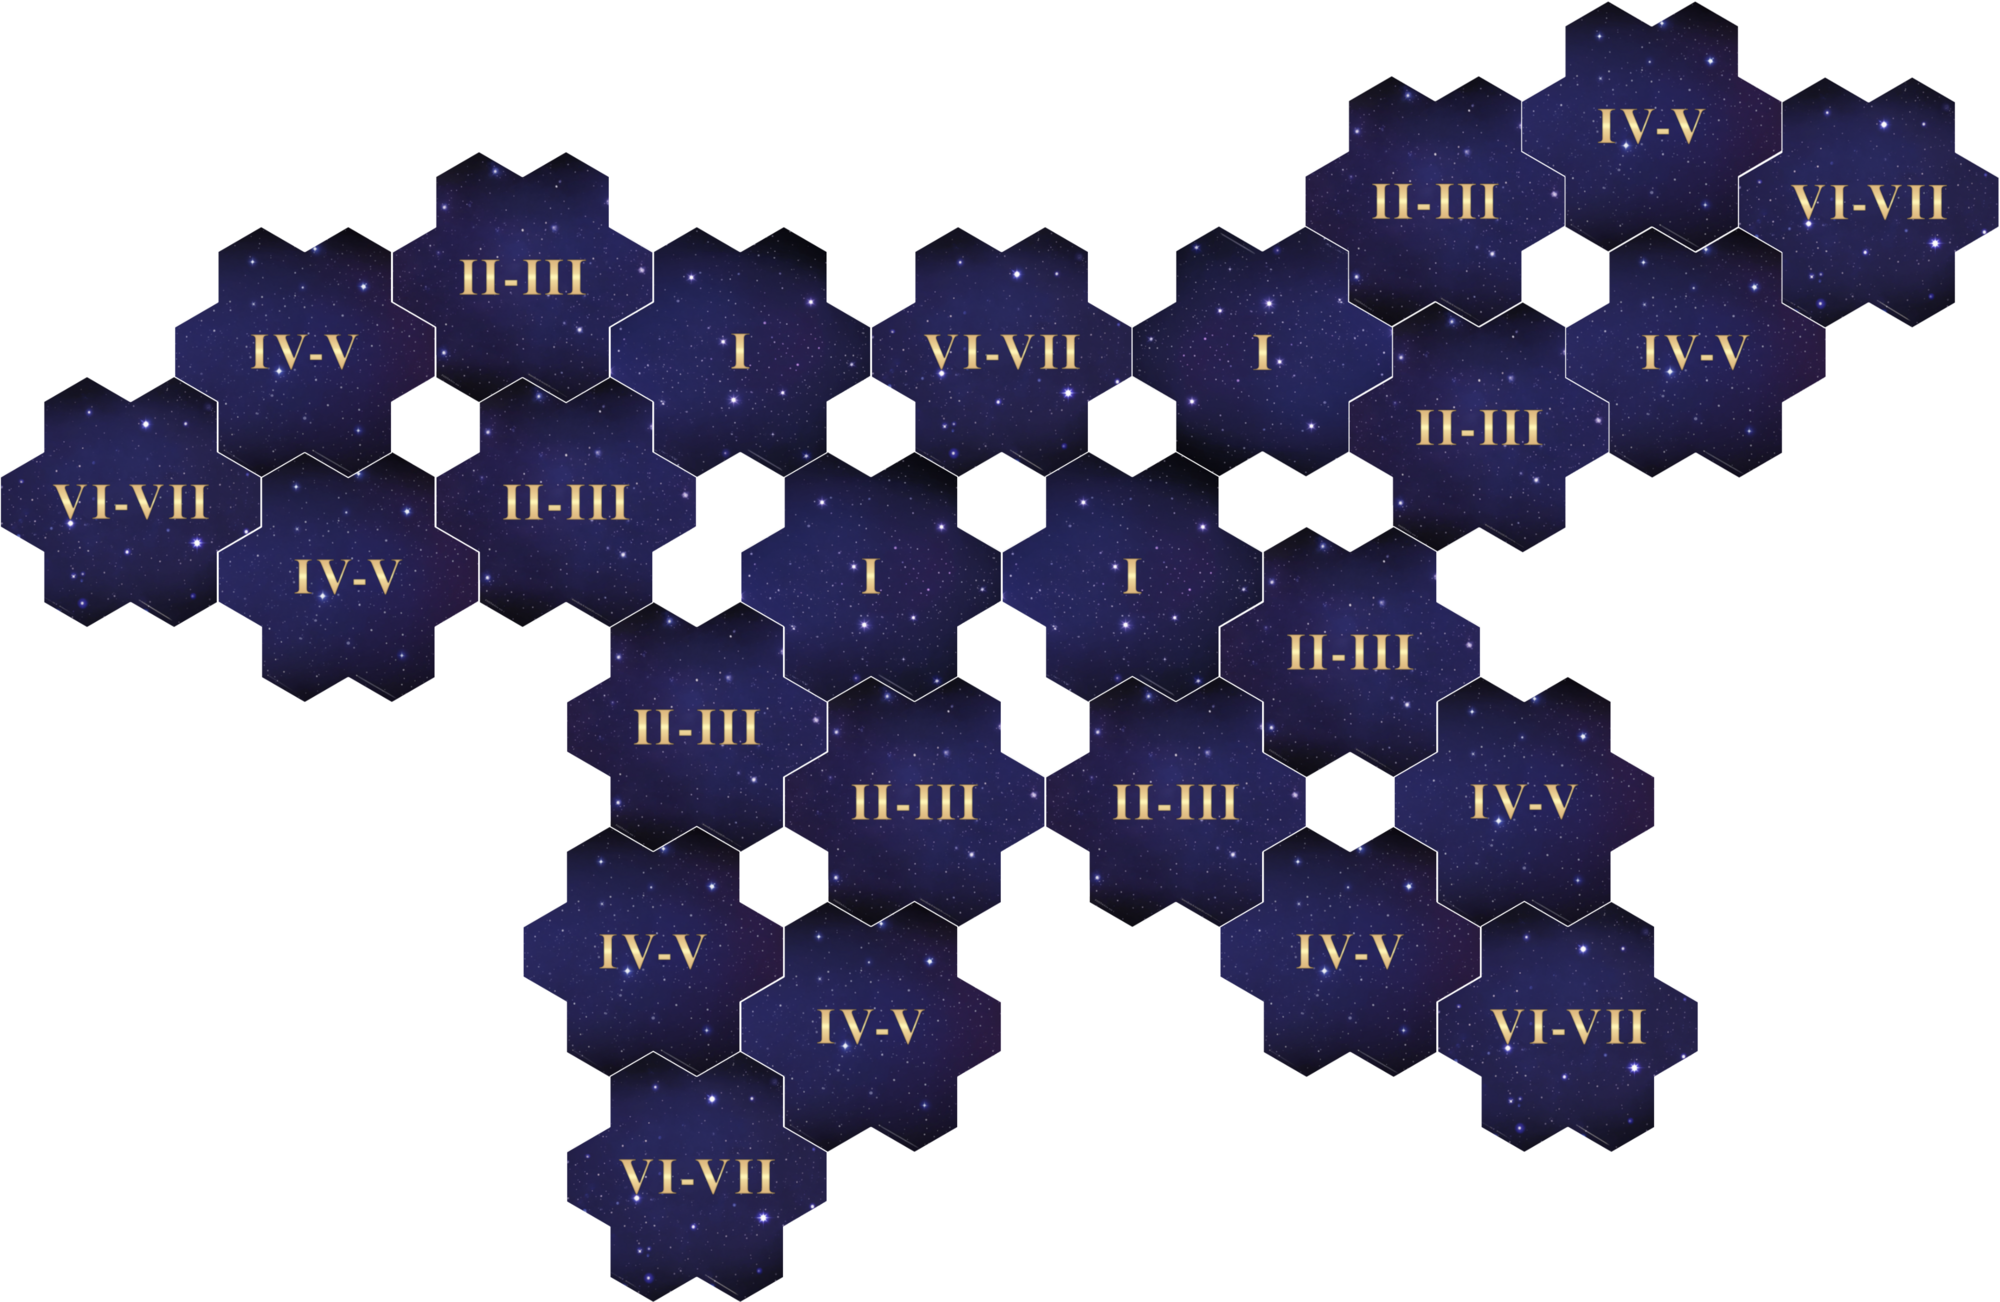
\includegraphics[width=0.38\paperwidth]{\_assets/maps/titans-4.png}
  \captionof{figure}{4-PLAYER SCENARIO}
\end{minipage}
\vspace{1em}
\linebreak
\begin{minipage}{0.4\paperwidth}
  \centering
  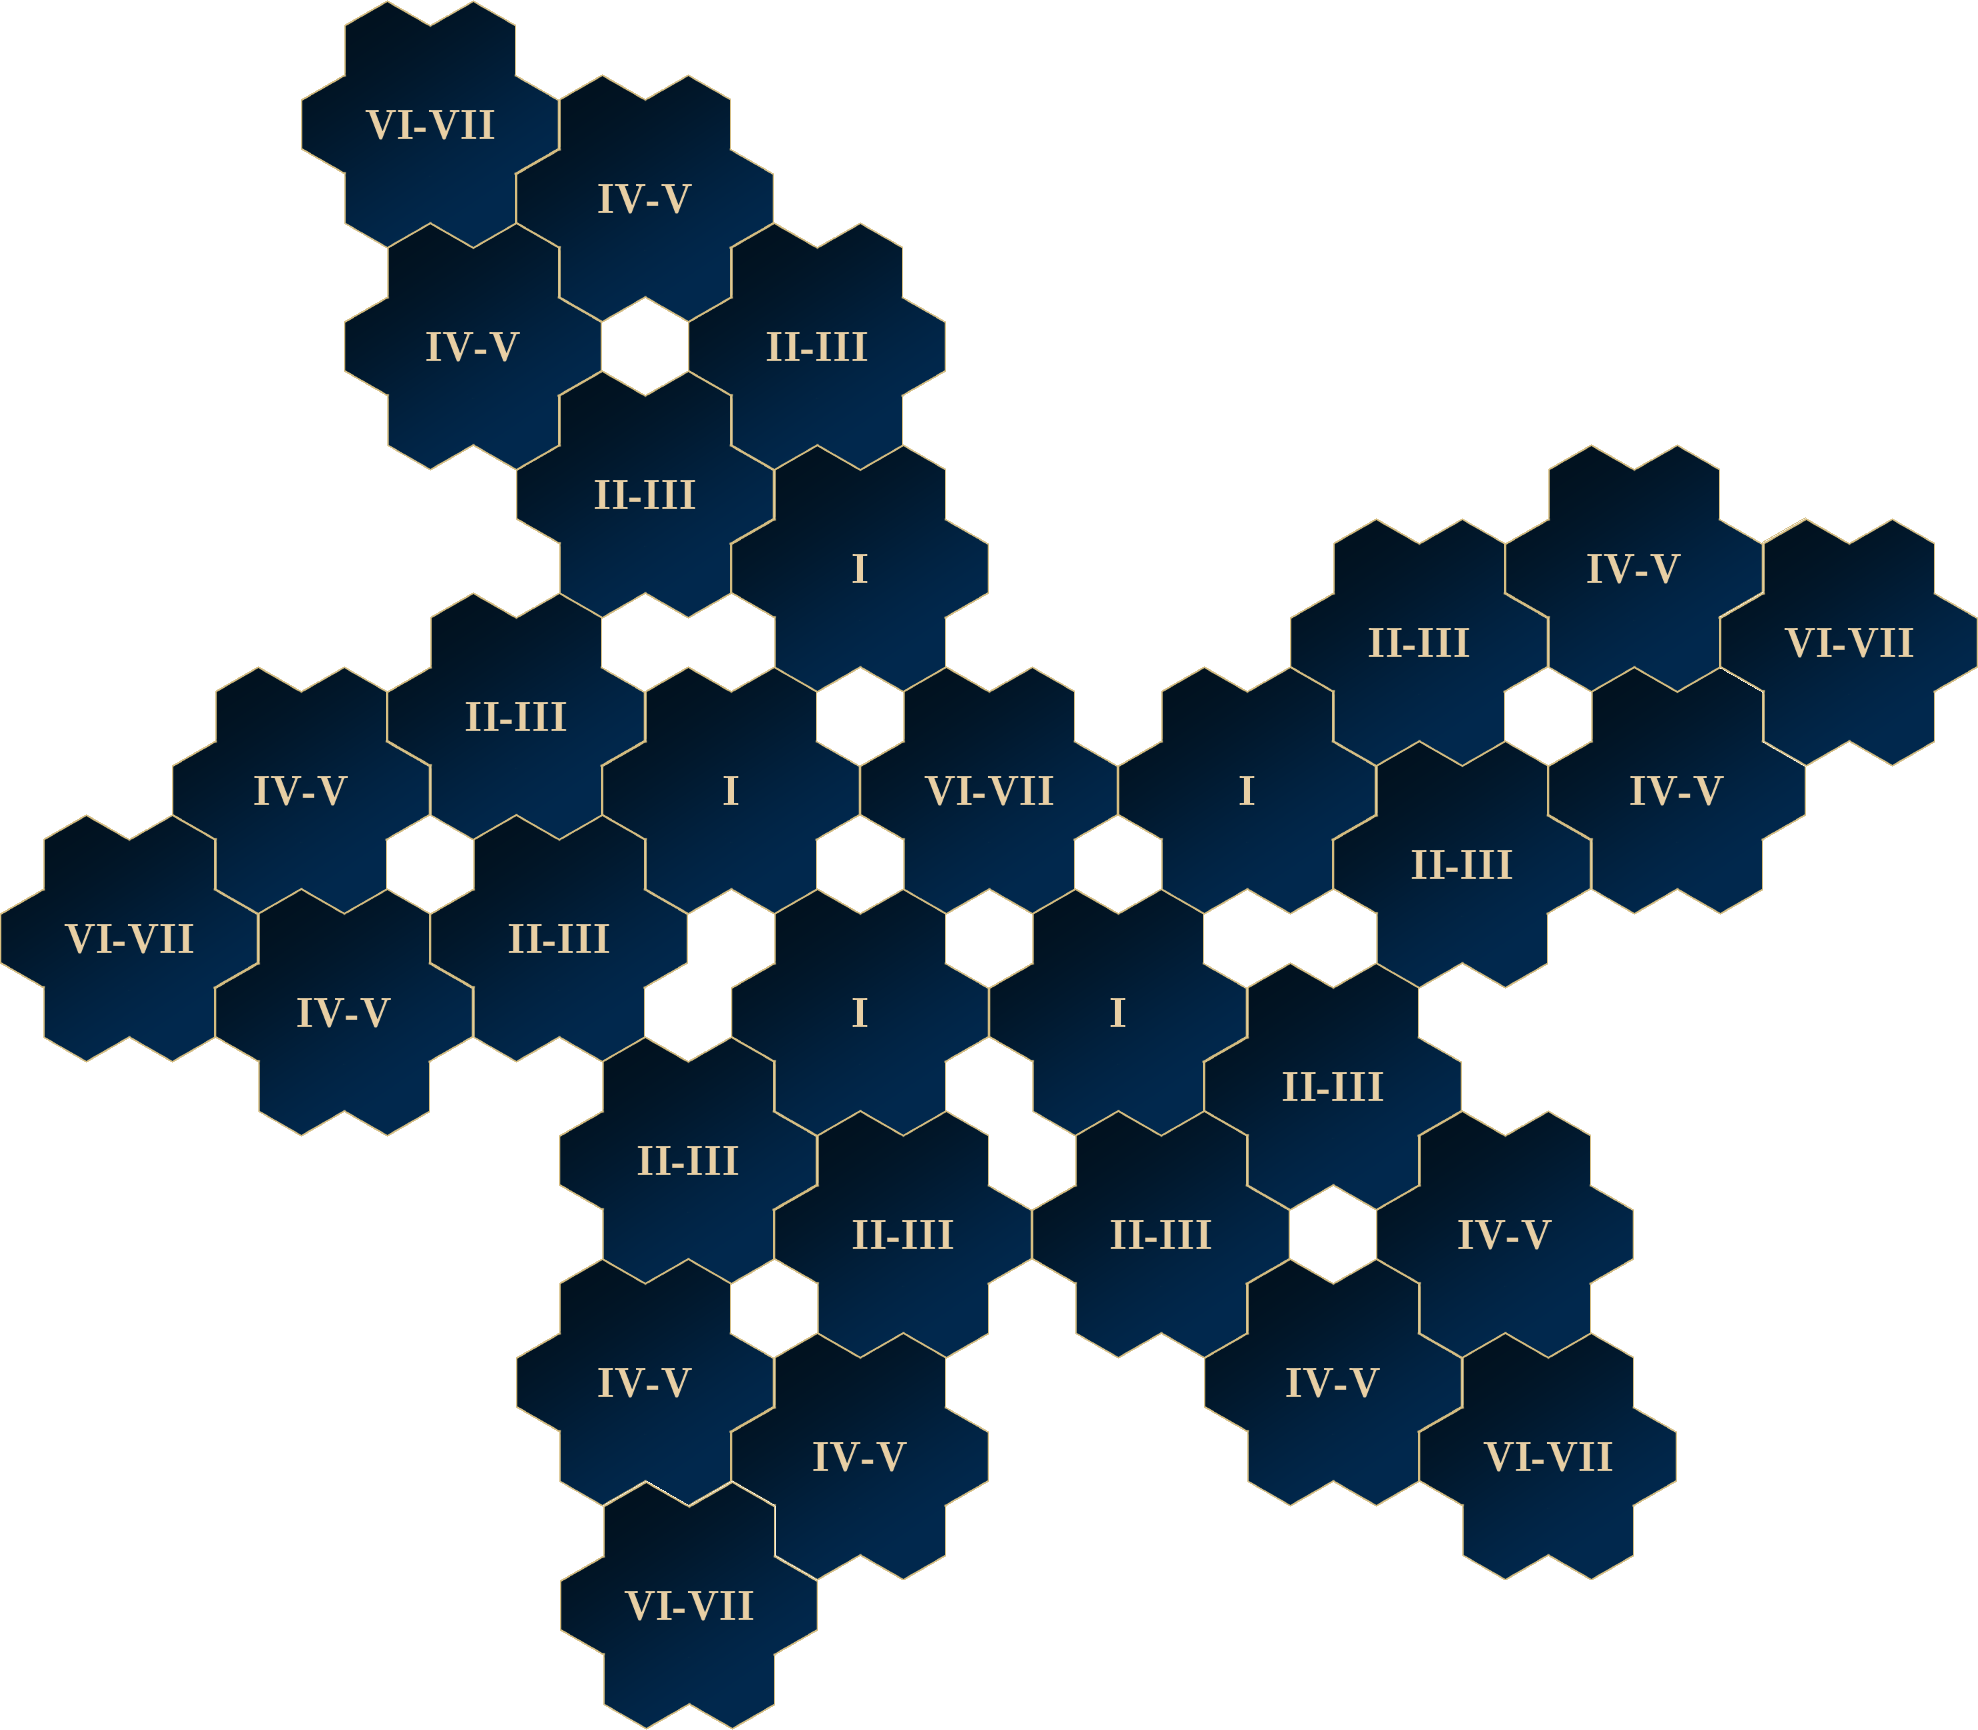
\includegraphics[width=0.38\paperwidth]{\_assets/maps/titans-5.png}
  \captionof{figure}{5-PLAYER SCENARIO}
\end{minipage}
\begin{minipage}{0.4\paperwidth}
  \centering
  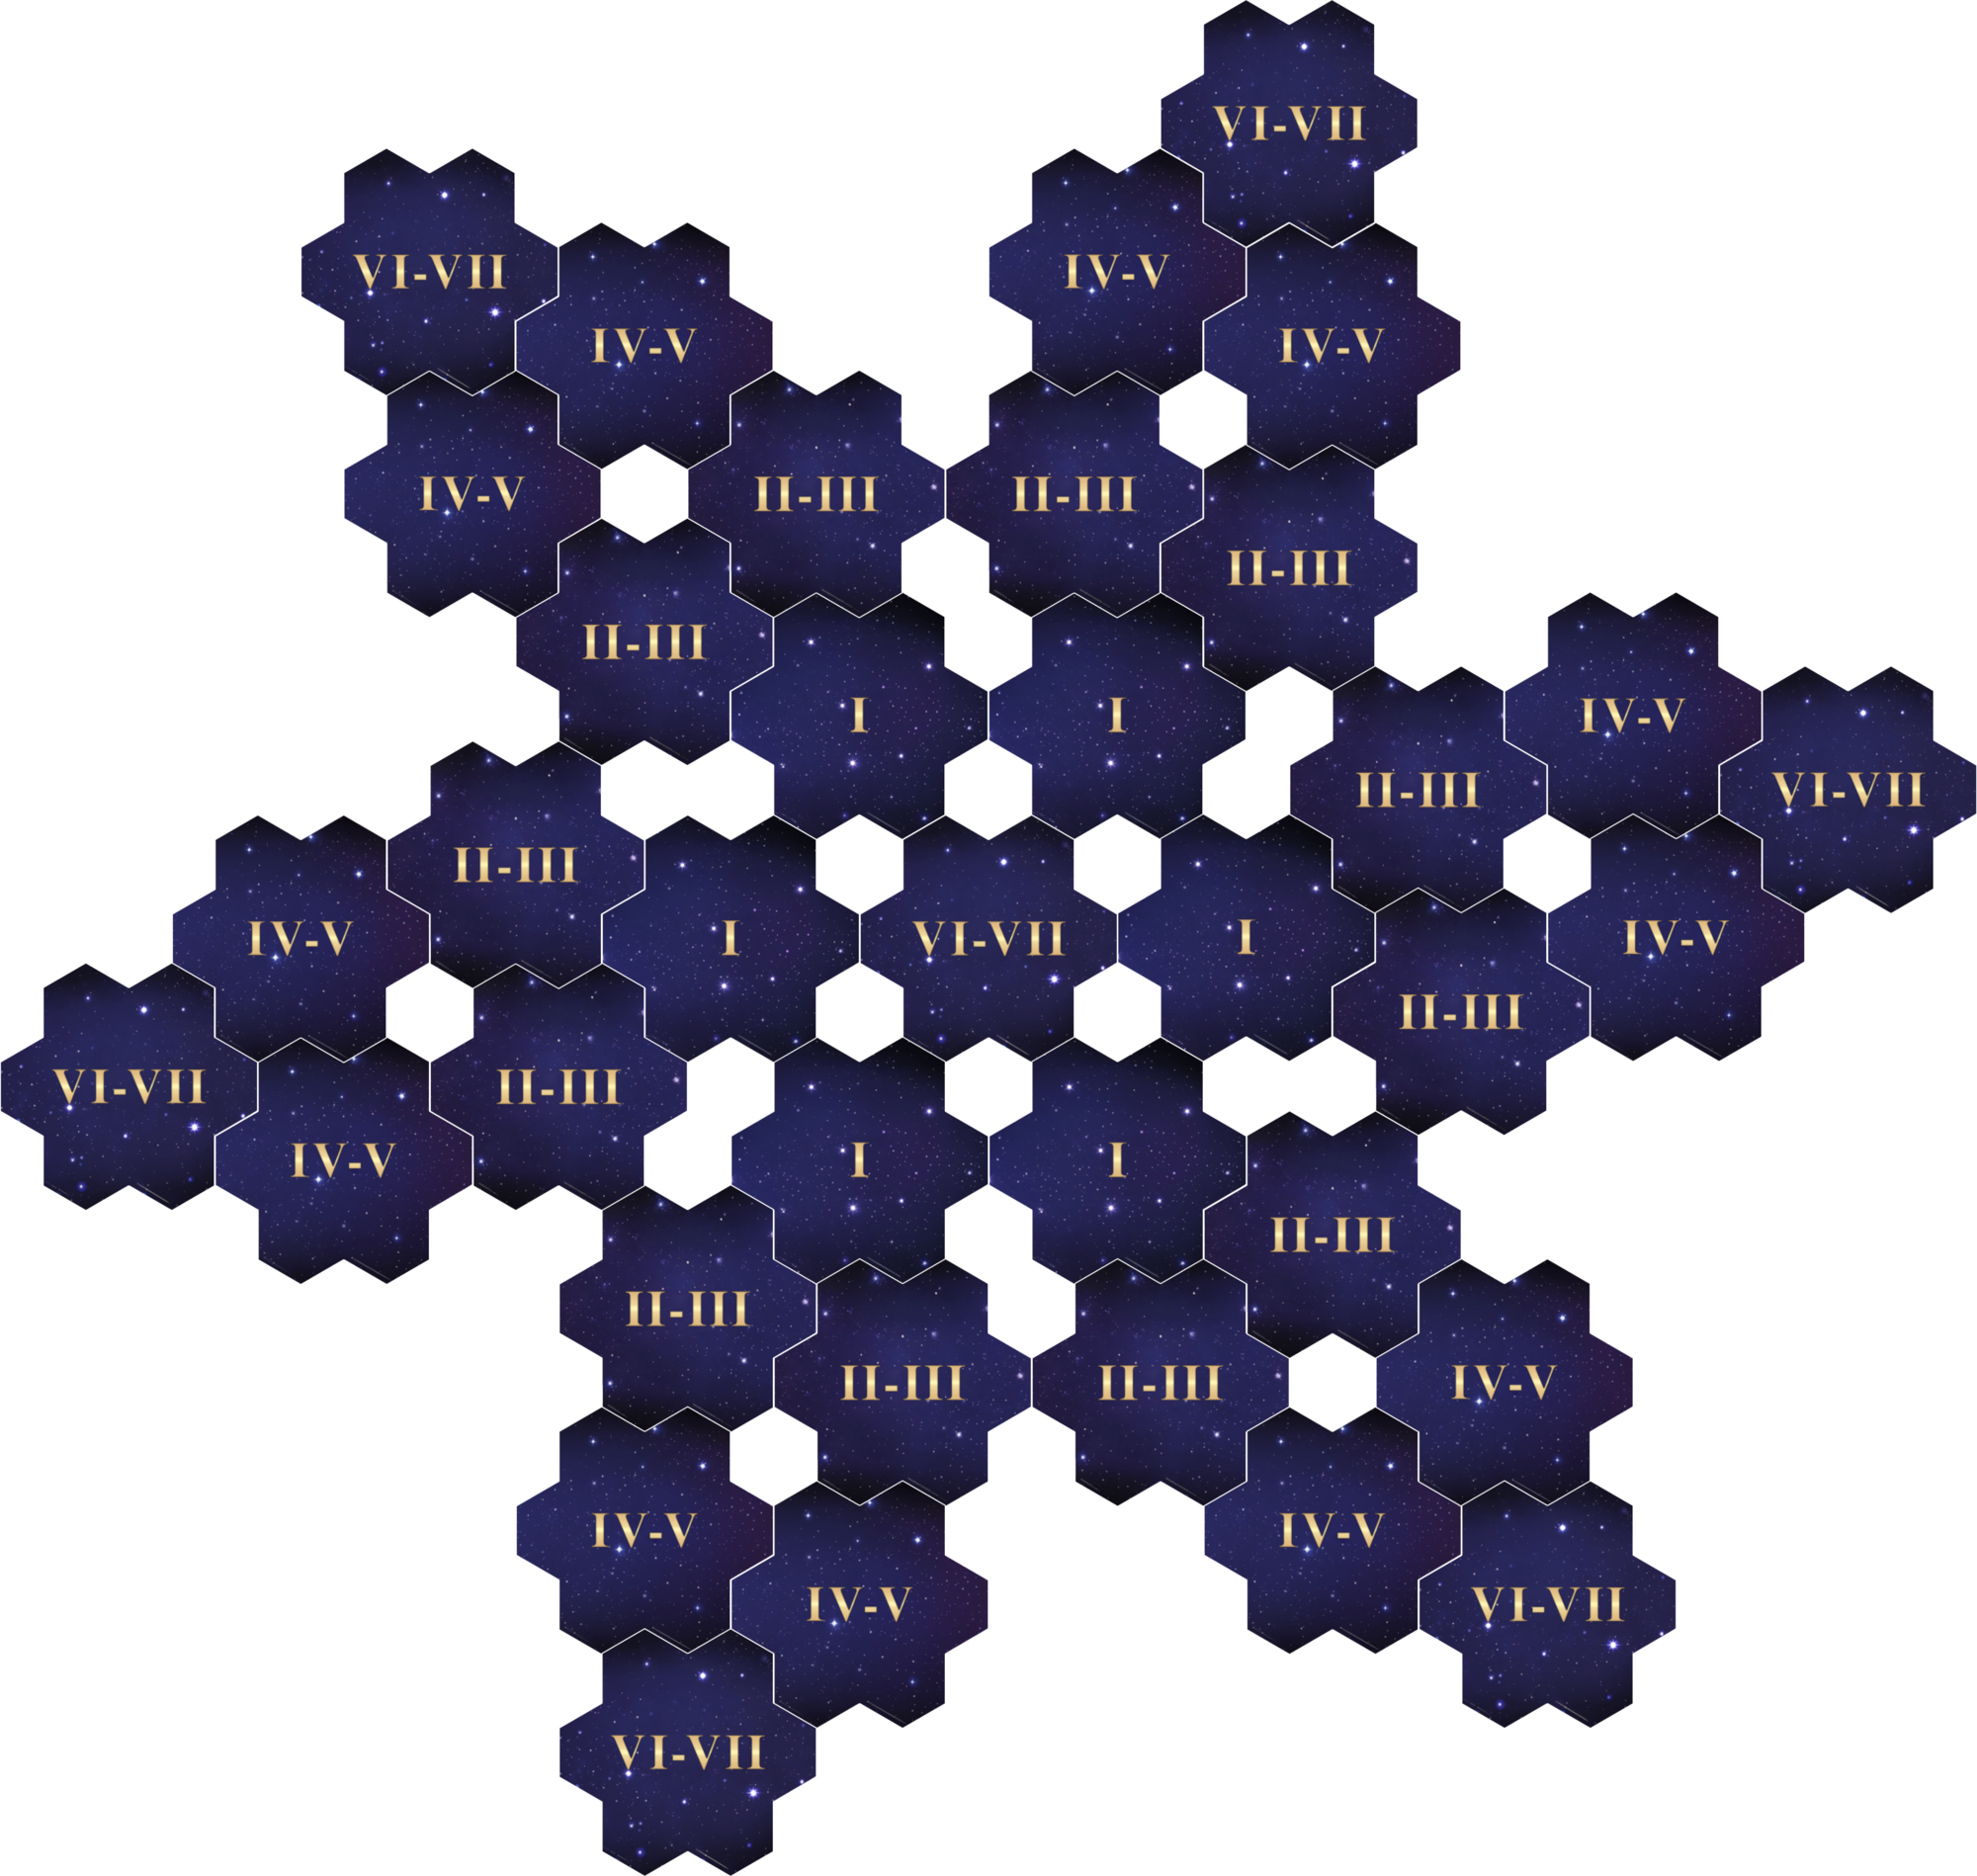
\includegraphics[width=0.38\paperwidth]{\_assets/maps/titans-6.png}
  \captionof{figure}{6-PLAYER SCENARIO}
\end{minipage}


\clearpage

% !TeX spellcheck = en_US
\addscenariosection{1}{Cooperative Scenario}{Emerald Island}{\images/logistics.png}

\begin{multicols*}{2}

\textbf{Author:} Invoceusse

\textbf{Source:} \href{https://discord.com/channels/740870068178649108/1222679455261261986}{Archon Studio Discord}

\textit{Lord Markham has decided to organize a treasure hunt and you and your friends are going to take part.
  But hurry up! Other teams are also on the trail, and one of them is almost finished!
  And above all, beware: it seems that a creature identified as a dragon lurks on this island!}
\subsection*{\MakeUppercase{Scenario Length}}

This Scenario is played over 8 Rounds.

\subsection*{\MakeUppercase{Player Setup}}

\textbf{Player Count:} 1 -- 4

\textbf{Starting Resources:} 5 \svg{gold}, 2 \svg{building_materials}, 1 \svg{valuables}

\textbf{Starting Income:} 10 \svg{gold}, 0 \svg{building_materials}, 1 \svg{valuables}

\textbf{Starting Units:}
\begin{itemize}
  \item A Pack of \bronze\ Units of your choice
  \item A Few \bronze\ Units of your choice
\end{itemize}

\textbf{Town Buildings:} \bronze\ Dwelling

\textbf{Map Tile Pool:} If you wish, you can distribute the II--III Tiles equally to each player rather than laying them out as proposed.

\textbf{Additional Bonus:} None

\subsection*{\MakeUppercase{Map Setup}}

Take the following Map Tiles and arrange them as shown in the Scenario map layout ($P$ stands for the number of players):

\begin{itemize}
  \item P × Starting (I) Map Tile
  \item 4P × Far (II--III) Map Tile
\end{itemize}

\subsection*{\MakeUppercase{Victory Conditions}}

Flag all Mines and Settlements. (Don't forget the Building Materials Mine in Tile I. Each Tile II--III contains one Mine or Settlement with a Level III fight.)

\subsection*{\MakeUppercase{Defeat Conditions}}

There are unflagged Mines or Settlements left in map at the end of Round 8.

\subsection*{\MakeUppercase{Timed Events}}

\textbf{\nth{5} Round:}
\begin{itemize}
  \item Gain again the result of one Field with a Black Cube.
\end{itemize}

\subsection*{\MakeUppercase{Additional Rules}}

\begin{itemize}
    \item Ignore any yellow lines between Tiles I (but not between Tiles I and Tiles II--III).

    \item You can't build a \golden\ Dwelling.

    \item You can give Units to another player, even outside your Turn, if one of your Heroes is:
    \begin{itemize}
        \item On the same Map Tile as another player's Hero.
        \item In another player's Town.
        \item Next to another player's Hero.
    \end{itemize}

    \item If you have no Units in your Unit Deck (after a battle or if you do not keep at least one Unit), return all your Units to your Faction's Unit pool (even if another player has one or more of your Units). This includes Units you've previously given to another player.

    \item When in another player's Town, you may Recruit or Reinforce their Units, either for them or for yourself. You need the other player's permission for it. Corresponding Dwellings or Citadel must be built to do so.

    \item For the last Mine/Settlement battle, add a \golden\ Neutral Unit. You have unlimited Turns for this battle. You can't use Expert Diplomacy to skip this battle!

    \item The first time you reach Level IV, gain your second specialty.

    \item When you reach Level IV, move your Token on the Level tracker to Level III.

    \item Additionally, no player can:
    \begin{itemize}
        \item Attack other Heroes.
        \item Capture a Mine or Settlement that is already Flagged.
    \end{itemize}
\end{itemize}

\vspace{2em}

\begin{center}
  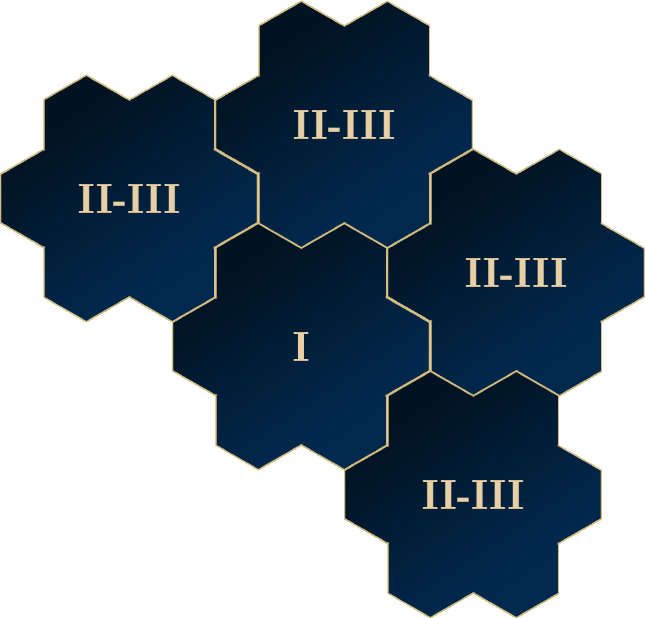
\includegraphics[width=0.2\paperwidth]{\maps/emerald-1.png}
  \captionof{figure}{\textbf{1-PLAYER SCENARIO}}
  \vspace{3em}
  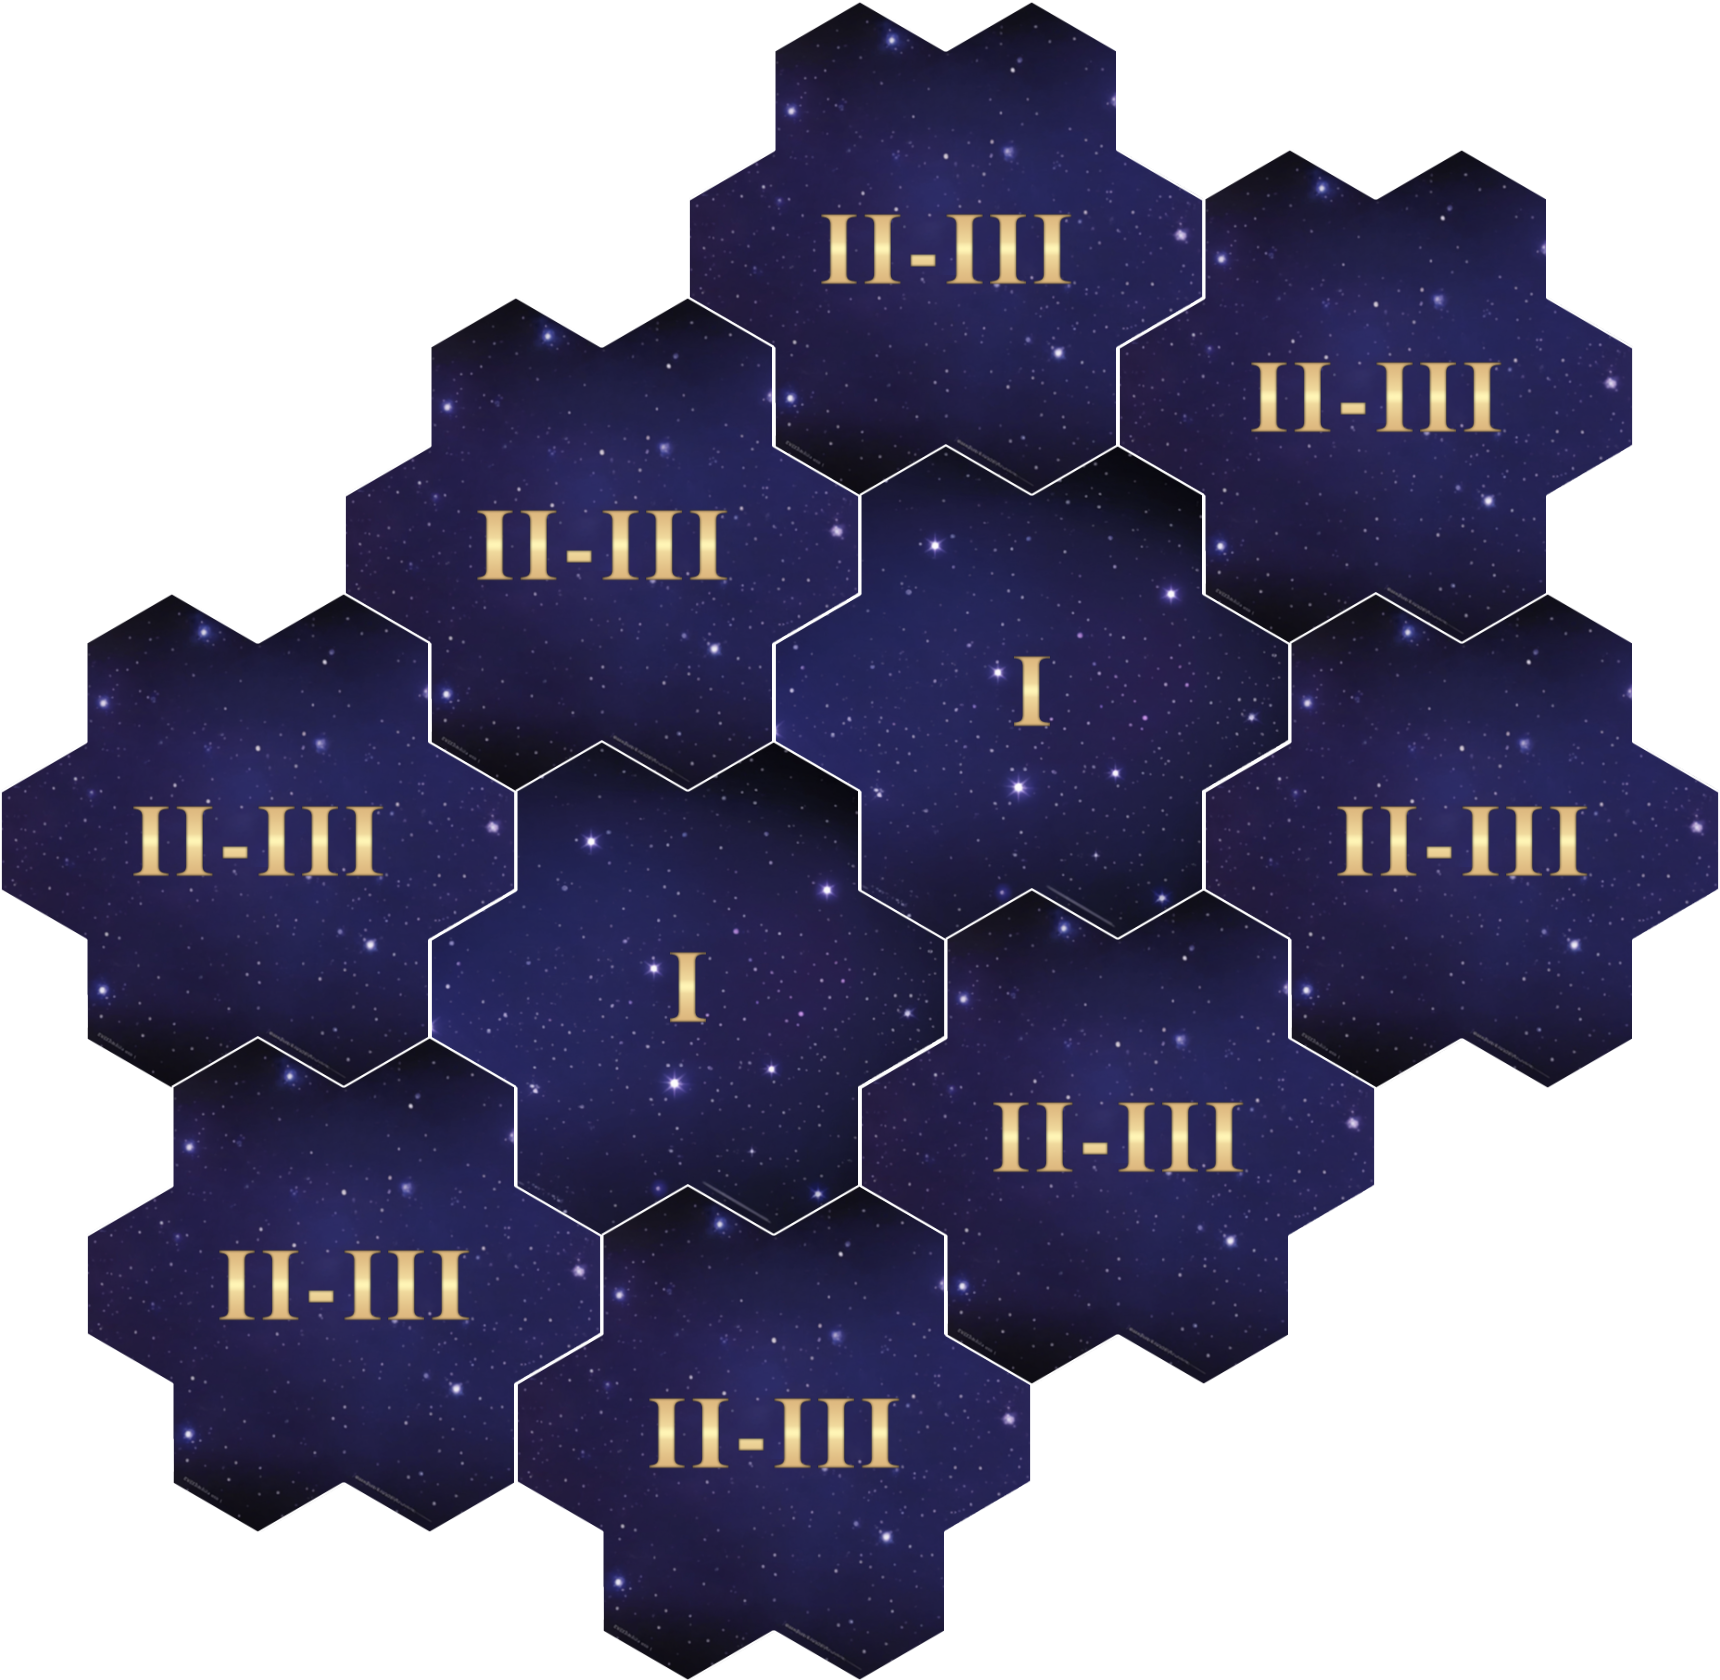
\includegraphics[width=0.3\paperwidth]{\maps/emerald-2.png}
  \captionof{figure}{\textbf{2-PLAYER SCENARIO}}
  \vspace{3em}
  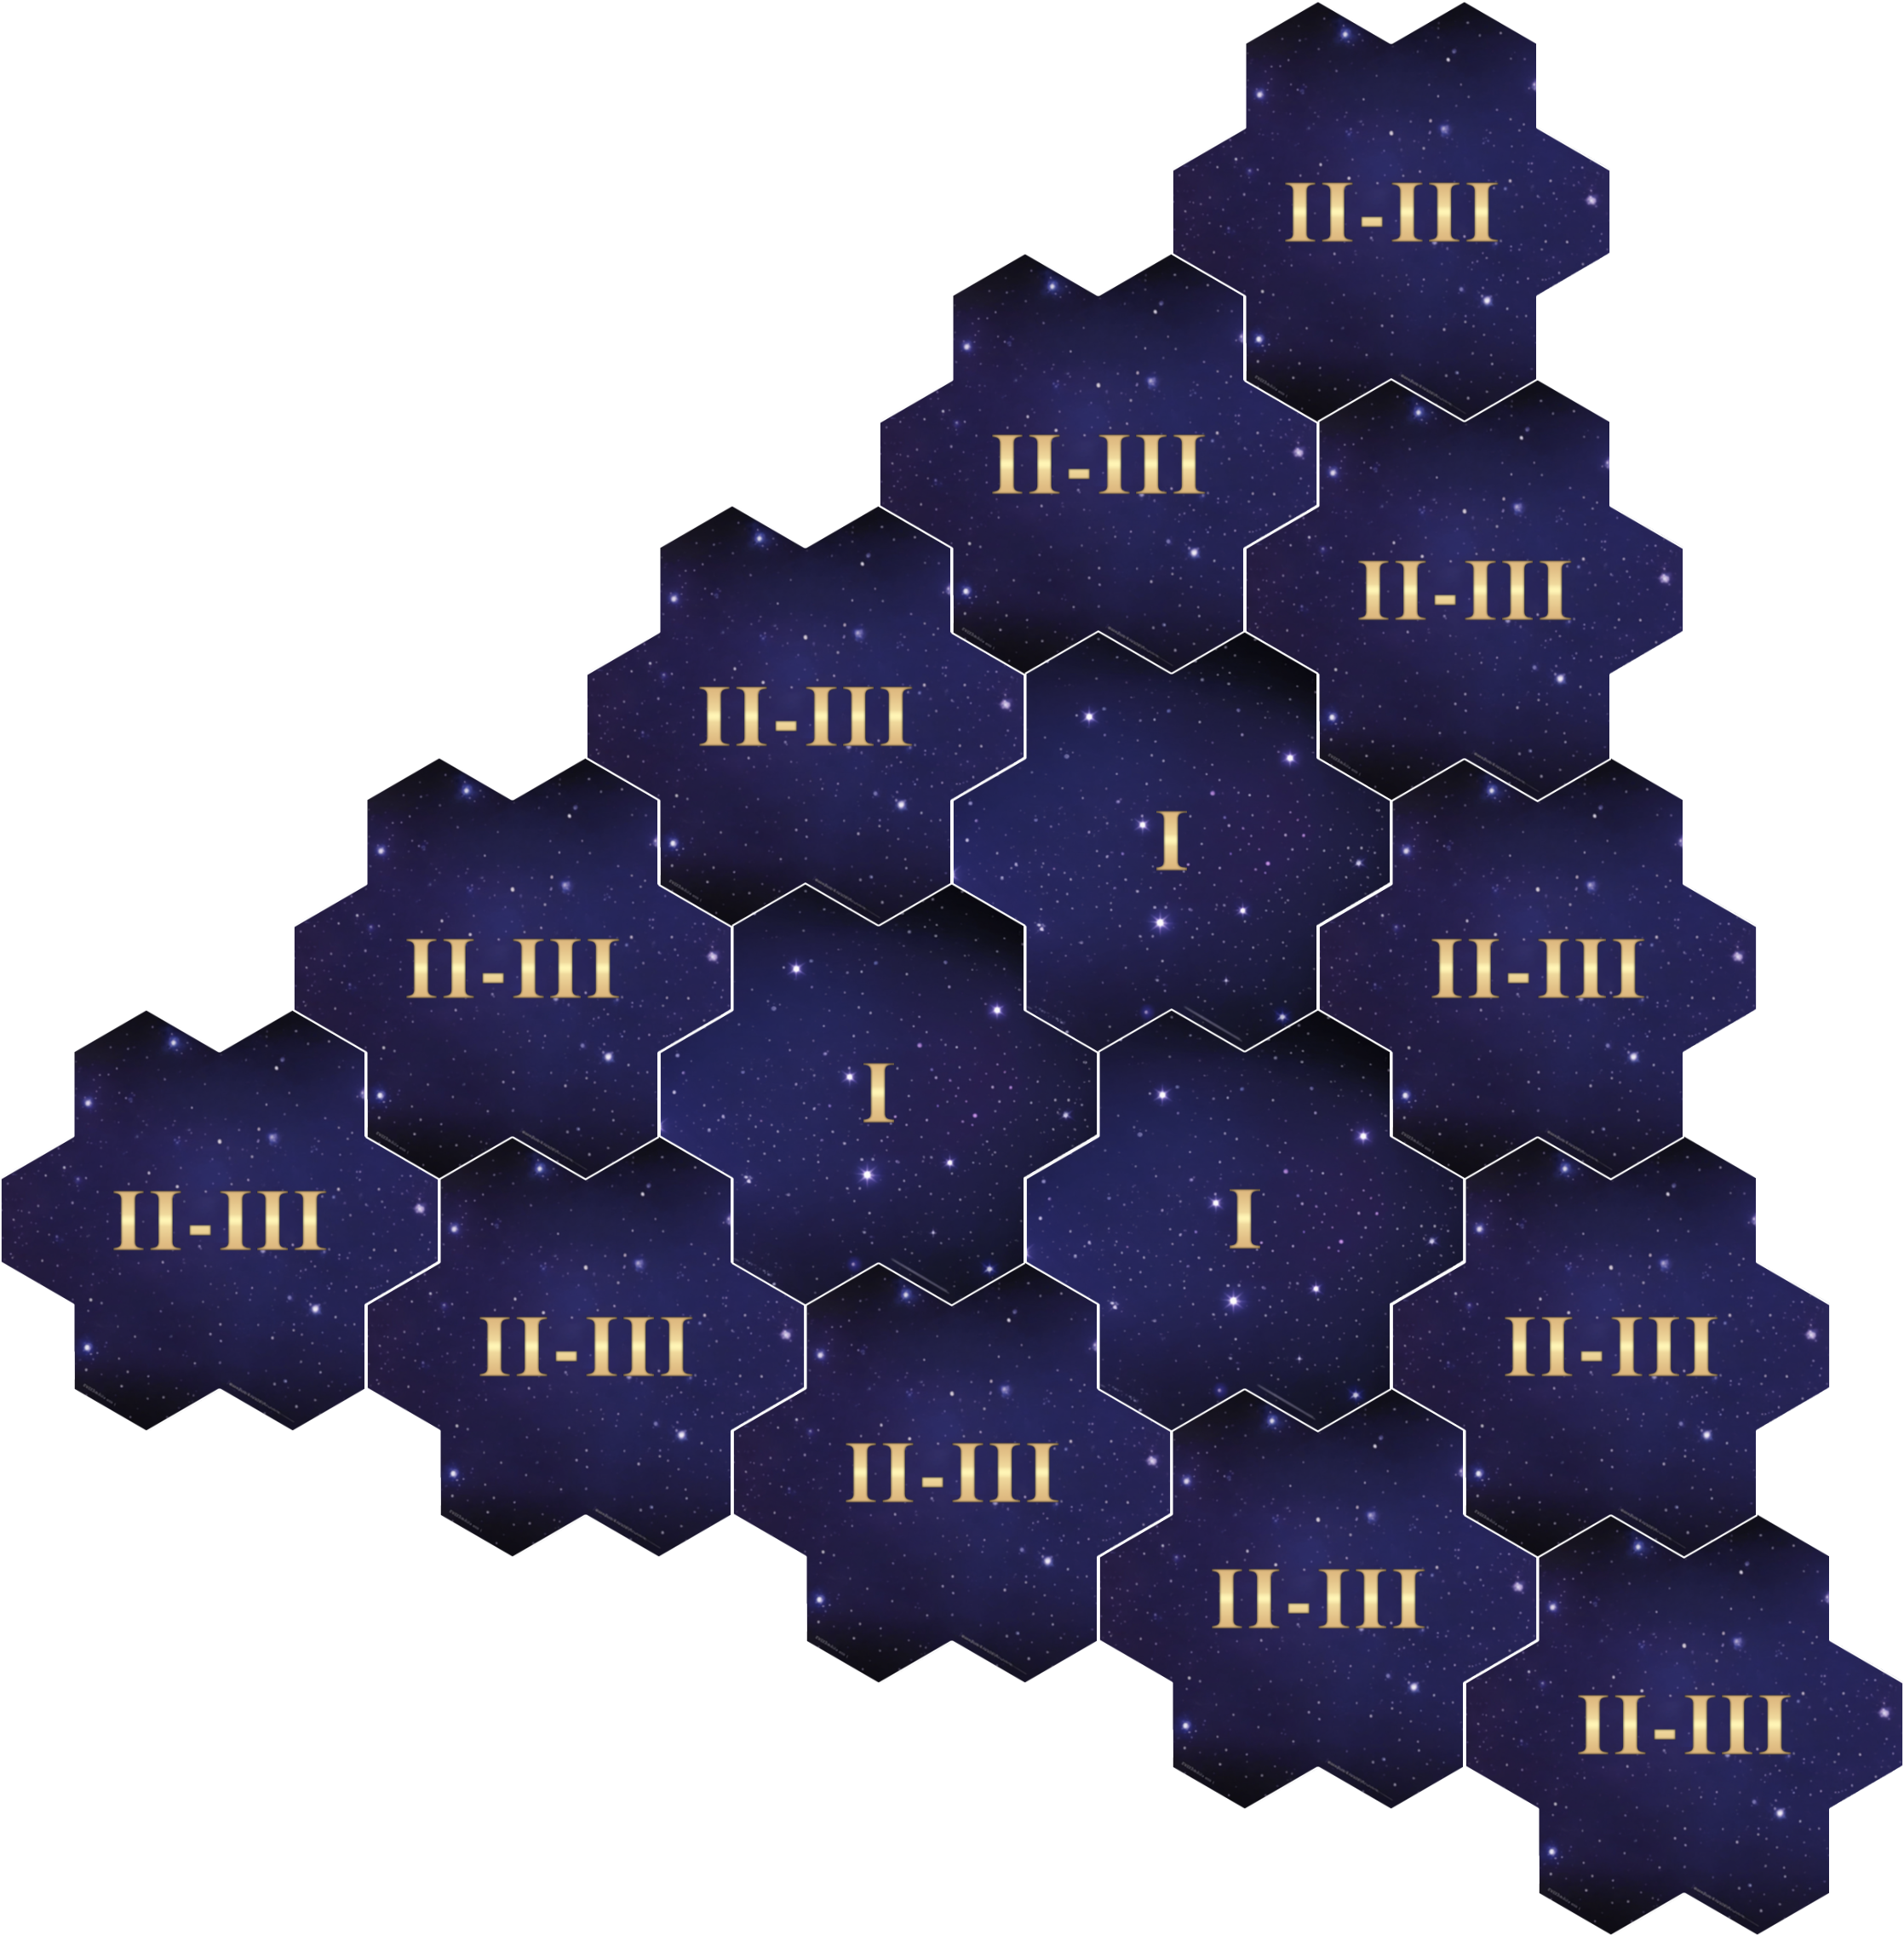
\includegraphics[width=0.3\paperwidth]{\maps/emerald-3.png}
  \captionof{figure}{\textbf{3-PLAYER SCENARIO}}
  \vspace{3em}
  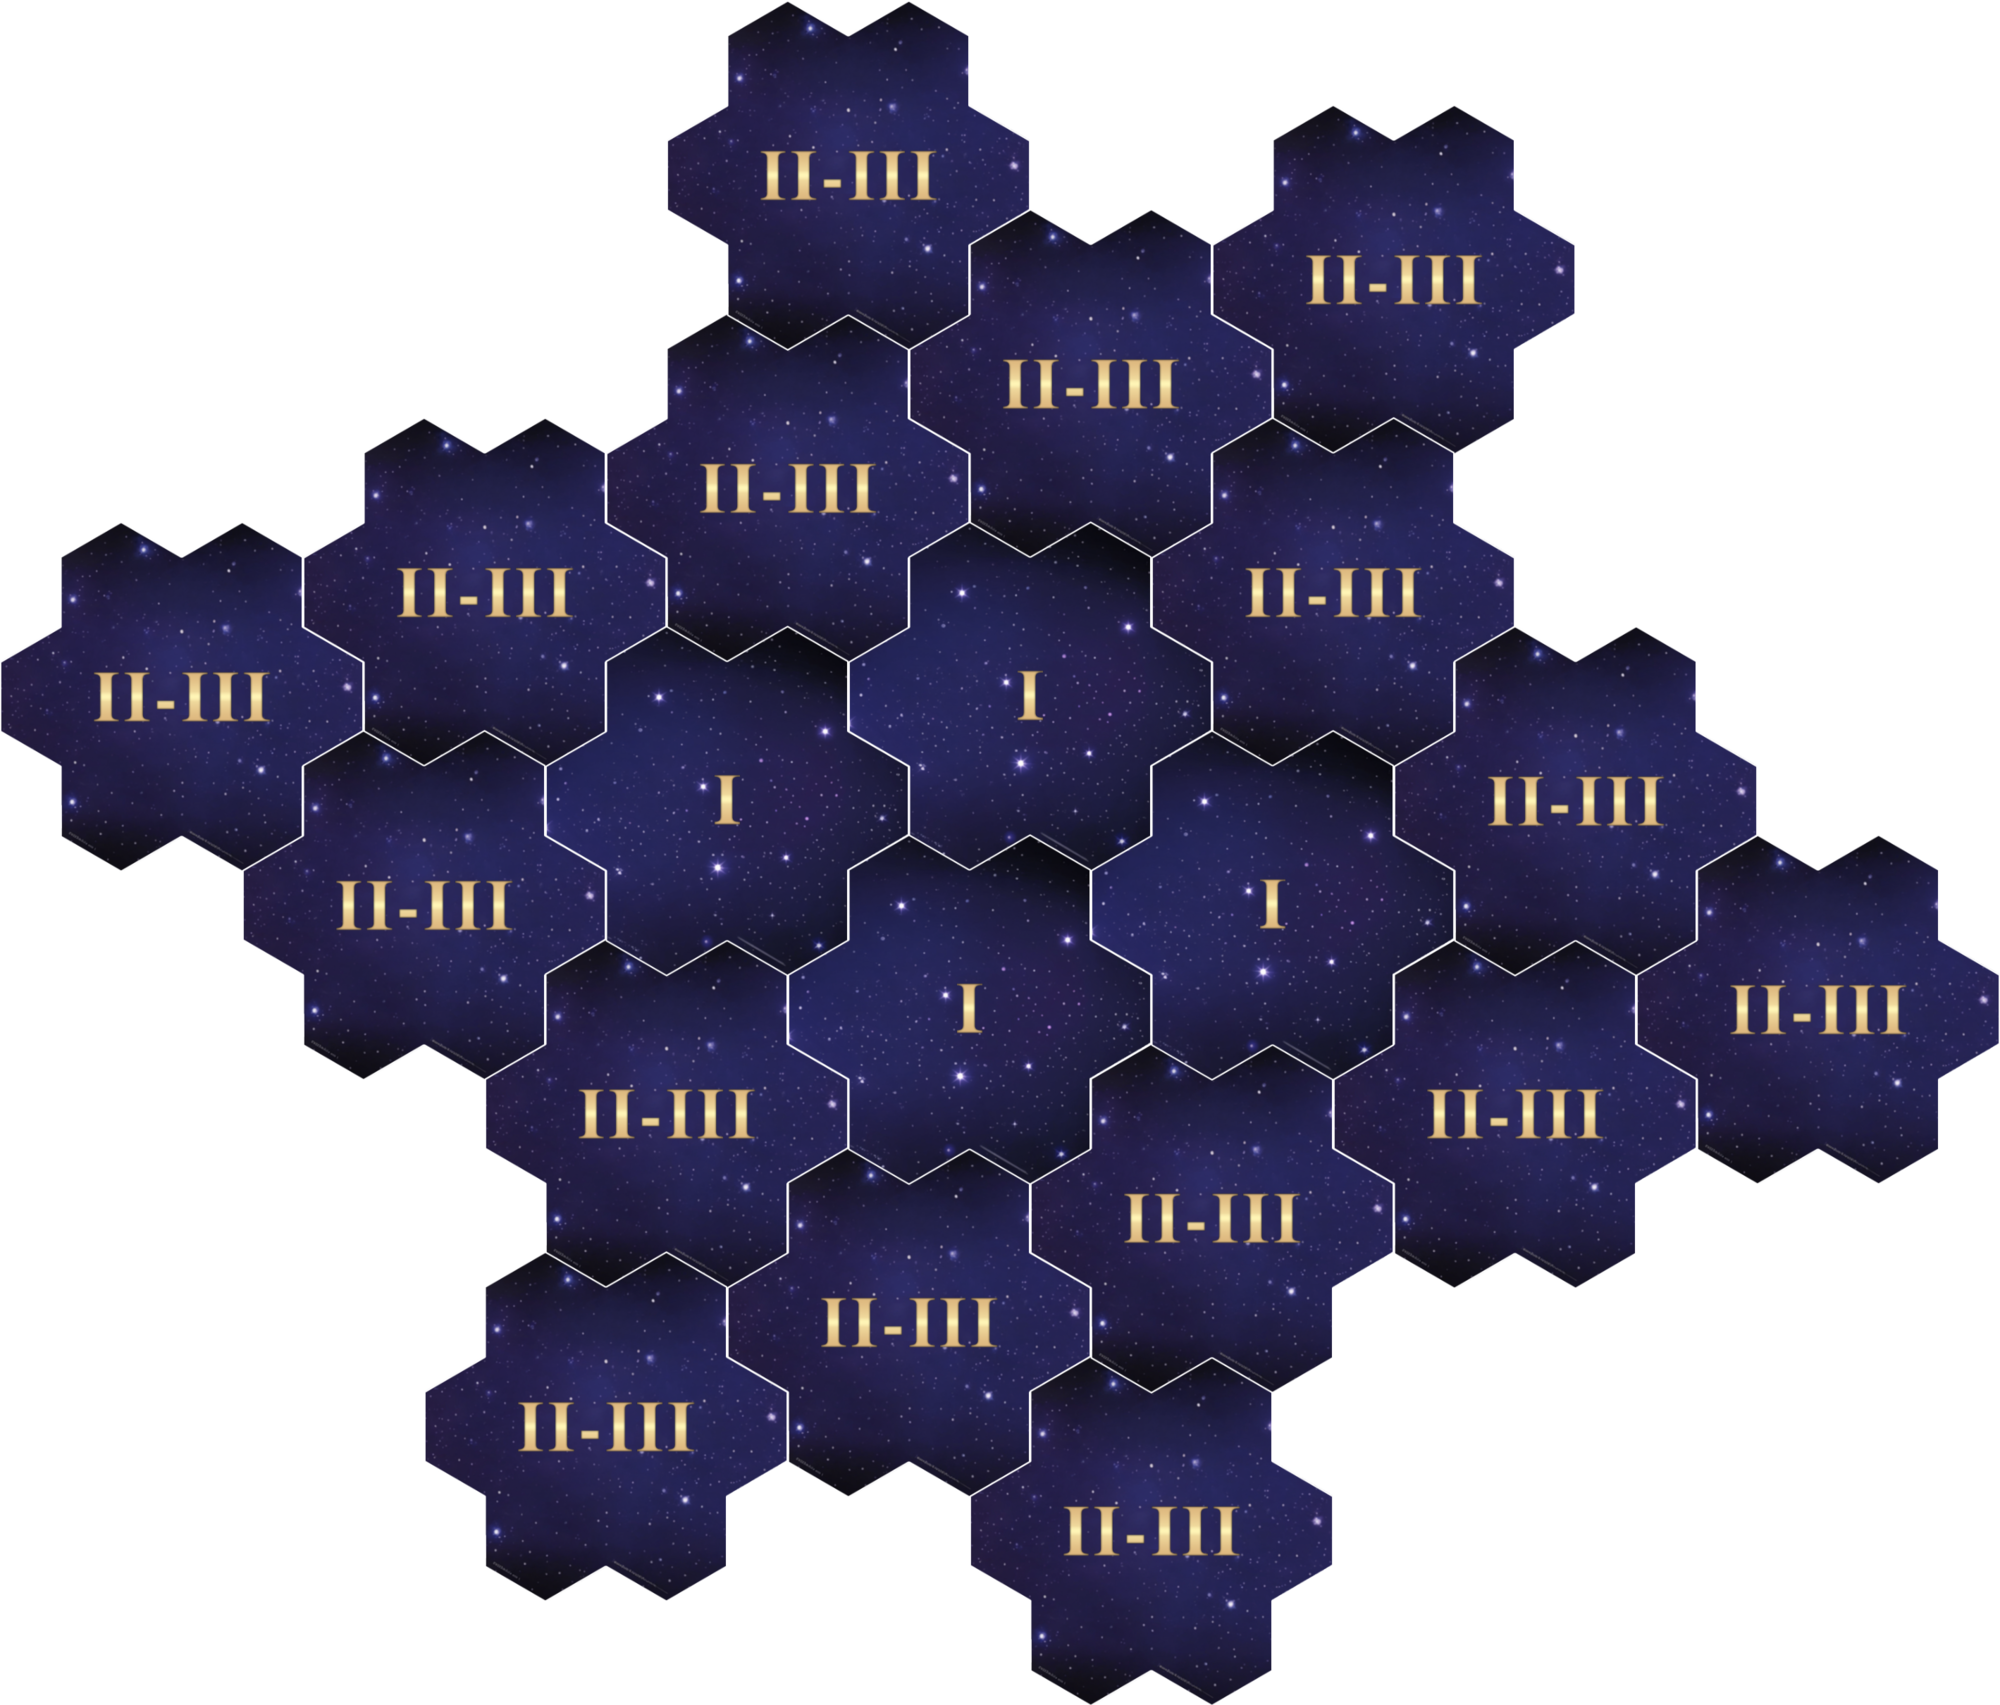
\includegraphics[width=0.3\paperwidth]{\maps/emerald-4.png}
  \captionof{figure}{\textbf{4-PLAYER SCENARIO}}
\end{center}

\end{multicols*}



\addscenariogroup{\clashtitle}{\layout/clash.png}

\clearpage

% !TeX spellcheck = en_US
\addscenariosection{1}{Clash Scenario}{Bloody Grail}{\images/bloody-grail.png}

\begin{multicols*}{2}

\textbf{Author:} Re4XN

\textbf{Source:} \href{https://discord.com/channels/740870068178649108/1239631918643941509}{Archon Studios Discord}

\textit{A Lady clad in dark robes visits you in your dreams, offering you a golden chalice full of blood-red wine. Waking up in a cold sweat, you decide to embark on a quest to find this unholy artifact.}

\subsection*{\MakeUppercase{Scenario Length}}
This scenario is played over 13 rounds.

\subsection*{\MakeUppercase{Player Setup}}
\textbf{Player Count:} 2 or 4

\textbf{Starting Resources:}\par
\resources{13}{2}{1}

\textbf{Starting Income:}\par
\resources{10}{0}{0}

\textbf{Starting Units:}
\begin{itemize}
  \item A Few \svg{bronze} units with the \textit{highest} Recruitment cost
  \item A Pack of \svg{bronze} units with the \textit{lowest} Recruitment cost
\end{itemize}

\textbf{Town Buildings:} \svg{bronze} Dwelling

\textbf{Map tile Pool:} Each player takes 2 random Far (II-III) Map tiles, one of which must contain a Settlement.

\textbf{Additional Bonus:} None

\subsection*{\MakeUppercase{Map Setup}}
Take the following Map tiles and set them up as shown in the scenario map layout:

\textbf{For a 2-player scenario:}
\begin{itemize}
  \item 2 × Starting (I) Map tile
  \item 4 × Near (IV-V) Map tile, all of which must contain an Obelisk
  \item 4 × Far (II-III) Map tile, 2 of which must contain a Settlement
  \item 1 × Center (VI-VII) Map tile, which must contain the Grail field
\end{itemize}

\textbf{For a 4-player scenario:}
\begin{itemize}
  \item 4 × Starting (I) Map tile
  \item 6 × Near (IV-V) Map tile, 4 of which must contain an Obelisk
  \item 8 × Far (II-III) Map tile, 4 of which must contain a Settlement
  \item 1 × Center (VI-VII) Map tile, which must contain the Grail field
\end{itemize}

\textbf{\MakeUppercase{Note:}} Before placing the Near tiles, separate them into 2 piles (with and without an Obelisk). Place them alternately so that the tiles with an Obelisk are not placed adjacent to each other.

\subsection*{\MakeUppercase{Victory Conditions}}
To win the scenario, a Hero must obtain the Grail token and bring it to their faction Town.

\subsection*{\MakeUppercase{Defeat Conditions}}
If the Grail is not obtained at least once by the end of the 13th round, the game ends, and all players lose the scenario.

If the Grail token has been obtained, the players gain additional time – until the end of the 16th round – to bring the Grail to their faction Town. Otherwise, all players lose the scenario.

\subsection*{\MakeUppercase{Timed Events}}
At the beginning of the 6th, 9th, and 12th rounds, remove all Black cubes from all Water Wheels and Windmills on the map. Additionally, all players possessing the title of ``\textcolor{darkcerulean}{Grail Knight}'' gain \svg{morale_positive}. Finally, any players who do not possess a title gain 2 \svg{morale_negative}.
\end{multicols*}

\subsection*{\MakeUppercase{Additional Rules}}
Before this scenario:

\begin{itemize}
  \item Split the Artifact deck by rarity into 3 separate decks (Minor, Major, and Relic). A player may gain only Minor Artifacts on Starting or Far tiles, Minor or Major Artifacts on Near tiles, and Major or Relic Artifacts on Center tiles.
\end{itemize}

During this scenario:

\begin{itemize}
  \item When a player Visits an Obelisk, they \textit{must} resolve one of the following effects:
  \begin{enumerate}[leftmargin=15pt]
    \item \textbf{[Cleanse]} The player receives one of the following boons, depending on how many Obelisks they have Visited:
    \begin{enumerate}
      \item \textbf{[1st Obelisk]} Roll 2 \svg{treasure} and choose 1 to resolve; then, gain \svg{morale_negative}.
      \item \textbf{[2nd Obelisk]} Increase your \svg{gold}, \svg{building_materials}, or \svg{valuables} income by 1 step.
      \item \textbf{[3rd Obelisk]} You gain a Secondary Hero. Place their model on this field. If you already have a Secondary Hero, gain 3 \svg{gold} instead. Then, choose one enemy player to discard 2 random cards from their hand.
      \item \textbf{[4th Obelisk]} Remove up to 4 cards from your hand, except Statistic cards; then, search each corresponding deck for a card of your choice and put it in your hand.
    \end{enumerate}
    \item \textbf{[Sacrifice]} Remove a * faction Unit card from your Unit deck in exchange for:
    \begin{enumerate}
      \item *\svg{bronze}: Gain 6 \svg{gold}, 3 \svg{building_materials}, and 1 \svg{valuables}. Additionally, if the Unit card was on the Pack side, \textbf{Search (4)} the Minor Artifact deck.
      \item *\svg{silver}: Gain 12 \svg{gold}, 6 \svg{building_materials}, and 2 \svg{valuables}. Additionally, if the Unit card was on the Pack side, \textbf{Search (3)} the Major Artifact deck.
      \item *\svg{golden}: Gain 18 \svg{gold}, 9 \svg{building_materials}, and 3 \svg{valuables}. Additionally, \textbf{Search (2)} the Relic card deck. Finally, if the Unit card was on the Pack side, \textbf{Search (2)} the \svg{azure} Unit deck; you may Recruit one of these Units for half the cost (rounded down).
    \end{enumerate}
  \end{enumerate}
  \item A player that chooses \textbf{Sacrifice} at an Obelisk gains the title of ``\textcolor{darkcandyapplered}{Blood Knight}.'' Place a red faction cube on their Hero portrait to mark this effect. A \textcolor{darkcandyapplered}{Blood Knight} may never choose the \textbf{Cleanse} option when Visiting an Obelisk.
  \item A player that chooses \textbf{Cleanse} at an Obelisk gains the title of ``\textcolor{darkcerulean}{Grail Knight}.'' Place a blue faction cube on their Hero portrait to mark this effect. A \textcolor{darkcerulean}{Grail Knight} may never choose the \textbf{Sacrifice} option when Visiting an Obelisk.
  \item When a player chooses \textbf{Sacrifice} at an Obelisk, place a number of faction cubes on the sacrificed Unit card and on the Obelisk field equivalent to the number of times the player has chosen the \textbf{Sacrifice} option. For example, if the player is sacrificing for the second time, place 2 faction cubes on the Unit card and 2 faction cubes on the Obelisk field.
  \item A player who possesses the title of ``\textcolor{darkcerulean}{Grail Knight}'' may, after Visiting an Obelisk, recruit an enemy Unit sacrificed at that Obelisk for half the cost (rounded down); if a Pack was sacrificed, the player may choose to recruit Few instead.
  \item If a Unit recruited at an Obelisk is defeated, Remove it.
  \item A player who possesses no title or the title of ``\textcolor{darkcandyapplered}{Blood Knight}'' may not use the Diplomacy Ability card. If a player who possesses no title or the title of ``\textcolor{darkcandyapplered}{Blood Knight}'' draws the Diplomacy Ability card, they may show it to the other players, then discard it and draw a new Ability card in its stead.
  \item A player who possesses the title of ``\textcolor{darkcerulean}{Grail Knight}'' may not use the Diplomacy Ability card to Recruit Neutral Azure Units.
  \item Whenever an Astrologers Proclaim or Event card that allows you to Recruit Neutral Units is drawn, ignore it, and draw a new Astrologers Proclaim or Event card.
  \item Players can use their Deck of Might \& Magic when paying gold to defend their faction Town.
  \item Ignore Combat encounters on the field with the Grail.
  \item Players may not Visit the field with the Grail token unless they have already Visited at least two Obelisks or the Grail token has been taken by any Hero at least once.
  \item To obtain the Grail token, a player’s Hero must spend 2 MPs on the field with the Grail.
  \item If a player does not possess the title of ``\textcolor{darkcandyapplered}{Blood Knight},'' they must Remove a faction Unit card from their Unit deck immediately after obtaining the Grail token. This effect can only occur once per player.
  \item If another Hero defeats the Hero with the Grail token, they also take the Grail token.
  \item If a Hero with the Grail token Surrenders, the Grail token is placed on the hex where the Hero Surrendered.
  \item If a Neutral army defeats the Hero with the Grail token, the Grail token is placed on the field where the Hero was defeated.
  \item If a Hero with the Grail token casts Town Portal or uses the Inferno faction Castle Gate building, the Grail token is placed on the hex where the spell was cast or the building used.
  \item The Grail token behaves like a Permanent card that does not count towards your hand limit and cannot be discarded; it grants the following effect when played: ``$\infty$ Once during each Combat, if the Hero is a \textcolor{darkcandyapplered}{Blood Knight}, discard a card to remove up to 2 \svg{damage-red} from your units and assign it to enemy units.''
  \item A Hero with the Grail token who possesses the title of ``\textcolor{darkcerulean}{Grail Knight}'' may pay 10 \svg{gold} or 3 \svg{valuables} at any Temple map location to cleanse the Grail. Place a blue faction cube on the Grail token to mark this effect.
  \item Once cleansed, the Grail token behaves like a Permanent card that does not count towards your hand limit and cannot be discarded; it grants the following effect when played: ``$\infty$ Once during each Combat round, if the Hero is a \textcolor{darkcerulean}{Grail Knight}, discard a card to remove up to 2 \svg{damage-red} from your units.''
\end{itemize}

\begin{tikzpicture}[overlay]
  \centering
  \node at (4.5, -5) {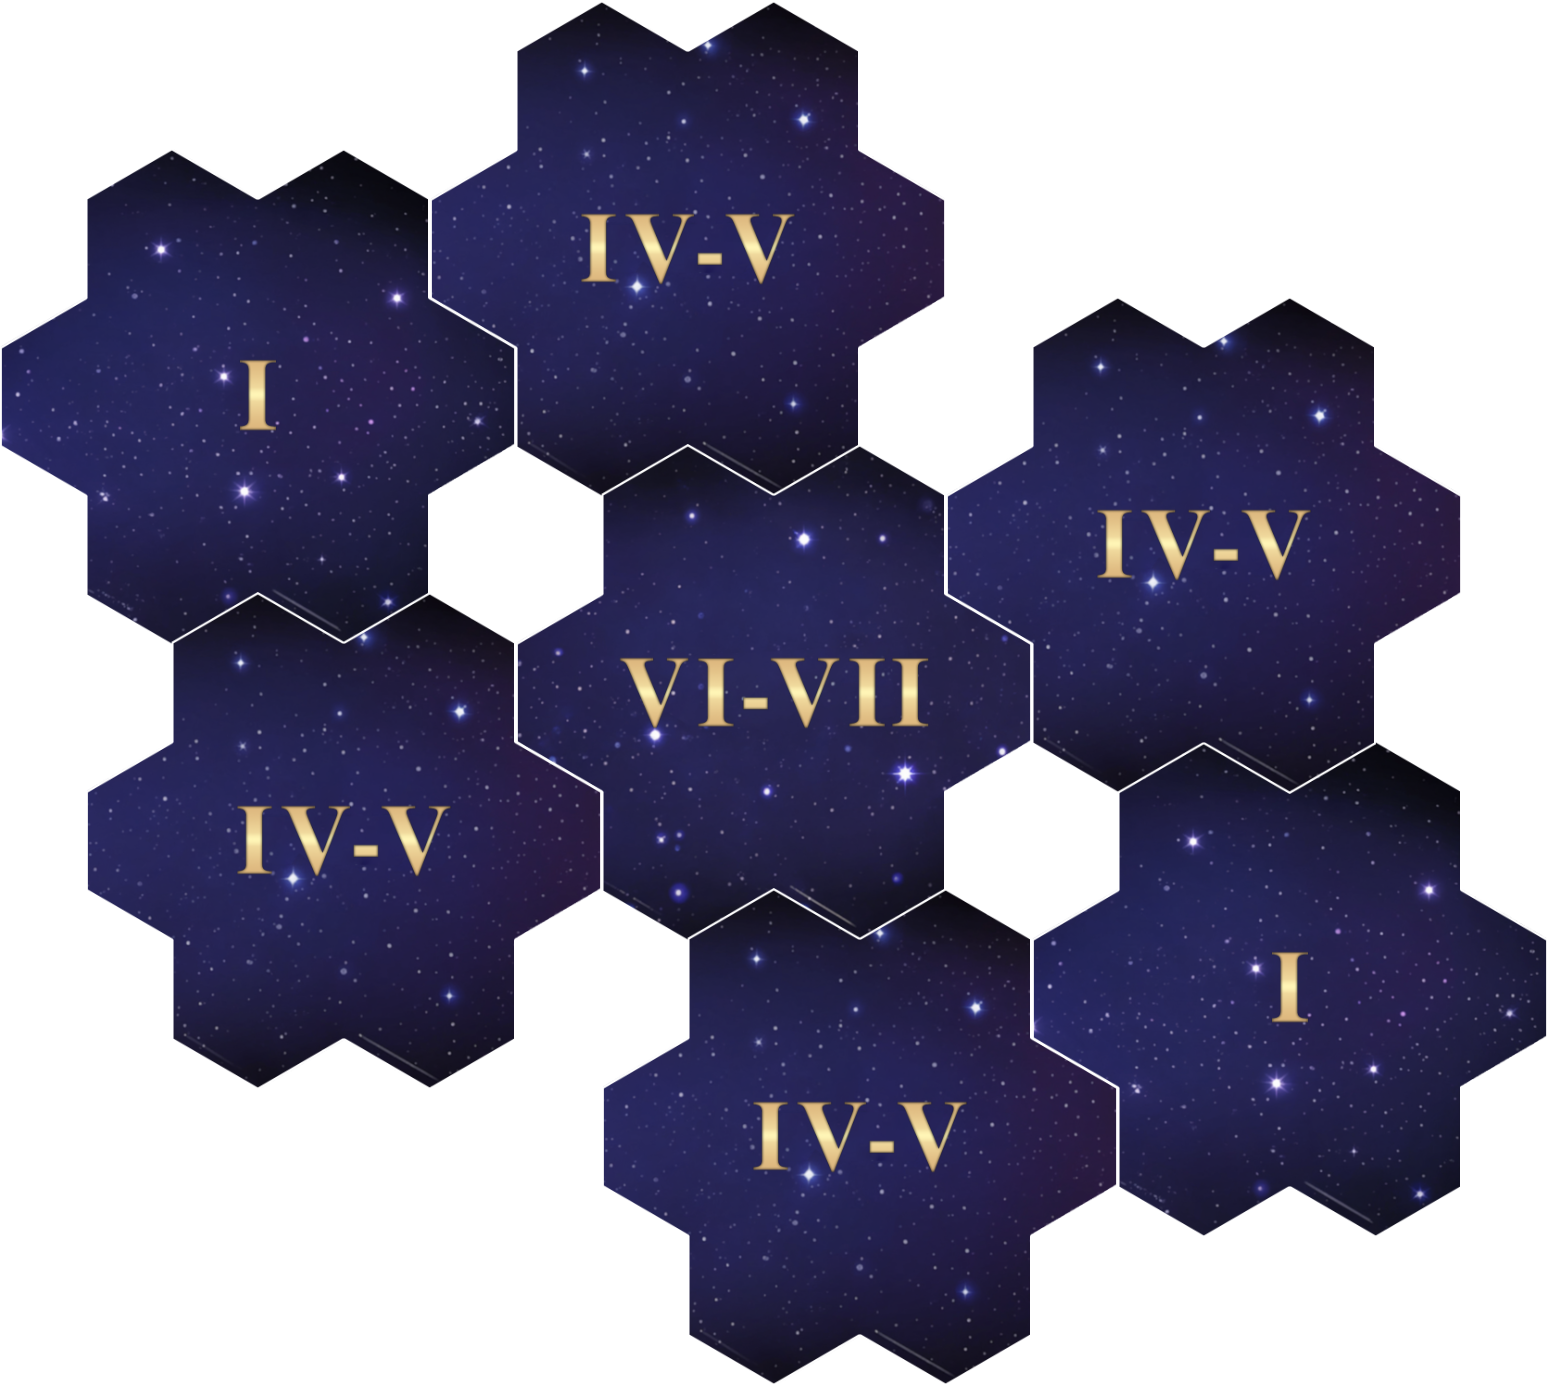
\includegraphics[scale=0.45]{\_assets/maps/bloody-grail-2p.png}};
  \node at (4.5, -10) {\footnotesize{\textbf{\MakeUppercase{2-PLAYER SCENARIO}}}};
  \node at (12.1, -14) {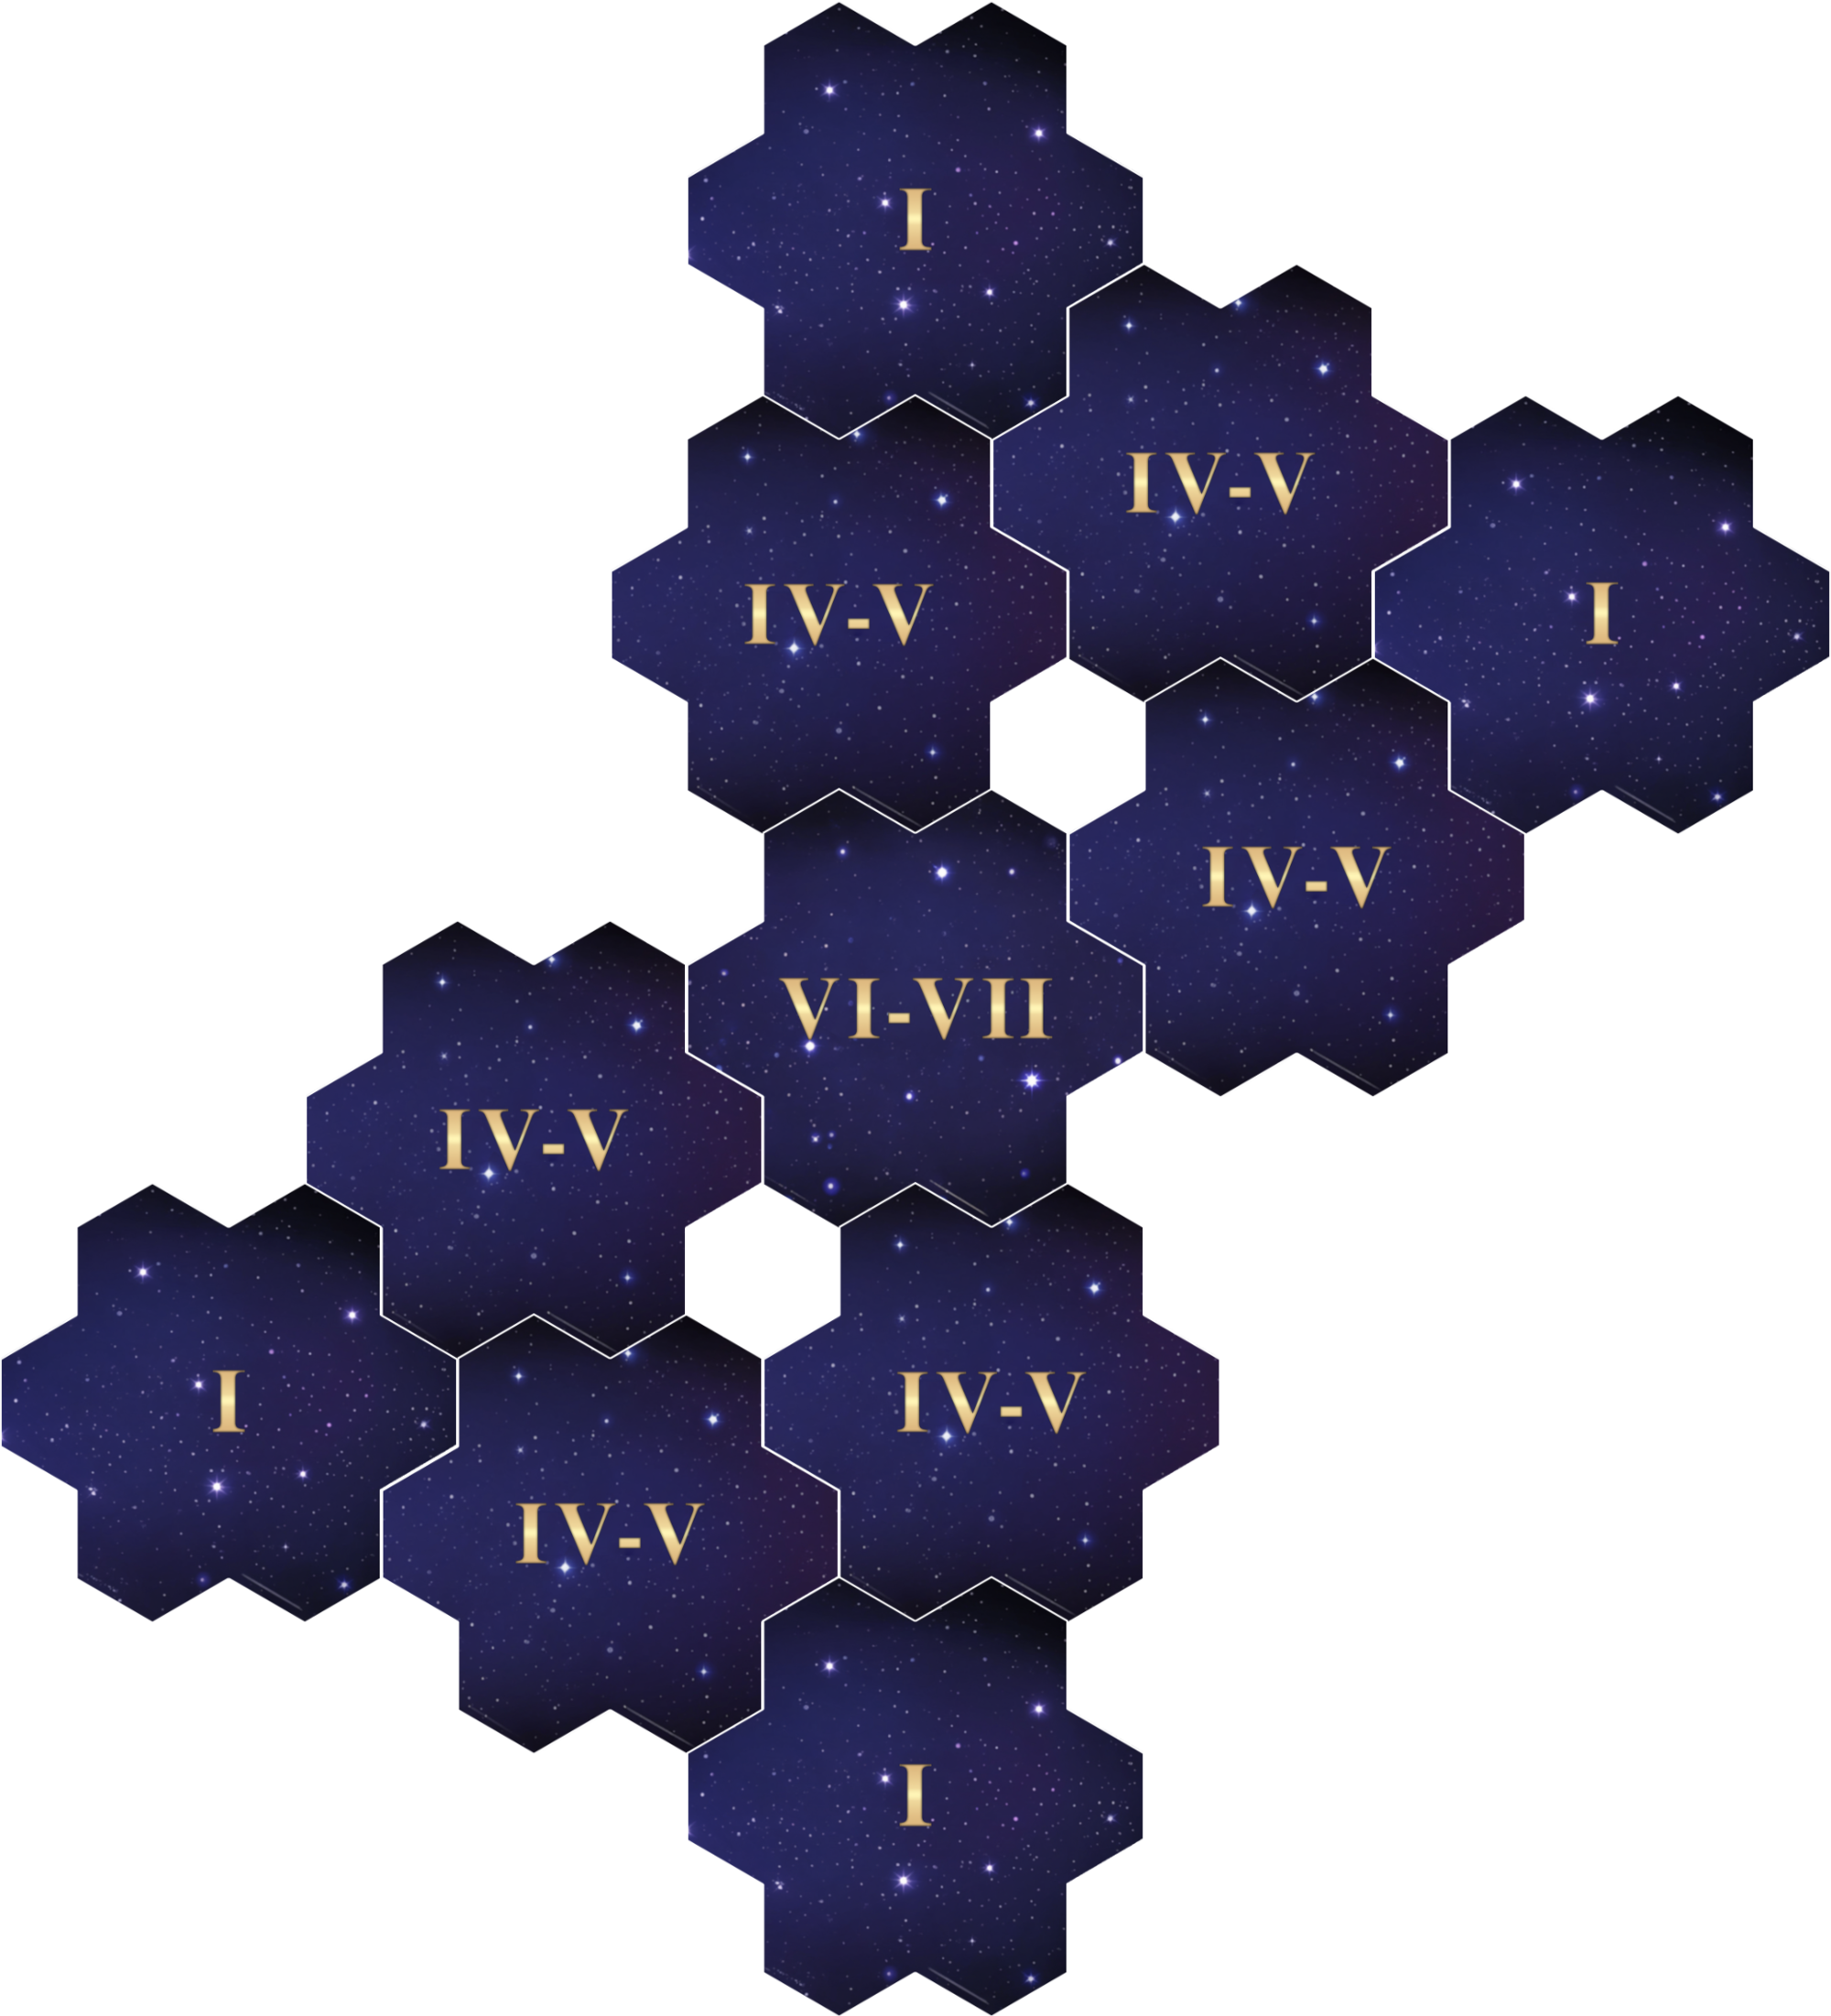
\includegraphics[scale=0.45]{\_assets/maps/bloody-grail-4p.png}};
  \node at (12.1, -21.6) {\footnotesize{\textbf{\MakeUppercase{4-PLAYER SCENARIO}}}};
\end{tikzpicture}


\clearpage

% % !TeX spellcheck = en_US
\addscenariosection{1}{Clash Scenario}{The Hunt}{\images/slayer.png}

\begin{multicols*}{2}

\textbf{Author:} Mateusz ``MATMOT'' Motyka

\textbf{Source:} \href{https://boardgamegeek.com/filepage/277736/clash-scenario-the-hunt-v10}{BoardGameGeek}

\textit{The land quivers under the reign of the fearsome Dragon.
  The one who dares to slay this monstrous beast shall ascend to the throne, crowned as the rightful ruler of the shattered kingdom.
}

\subsection*{\MakeUppercase{Scenario Length}}
This Scenario is played over 14 Rounds.

\subsection*{\MakeUppercase{Player Setup}}
\textbf{Player Count:} 2 or 3

\textbf{Starting Resources:} 15 \svg{gold}, 4 \svg{building_materials}, 2 \svg{valuables}

\textbf{Starting Income:} 10 \svg{gold}, 2 \svg{building_materials}, 1 \svg{valuables}

\textbf{Starting Units:}
\begin{itemize}
  \item A Pack of \bronze\ Units with the \textit{lowest} Recruitment cost
  \item A Few \bronze\ Units with the \textit{highest} Recruitment cost
\end{itemize}

\textbf{Town Buildings:} \bronze\ Dwelling, City Hall

\textbf{Map Tile Pool:} Each player takes 1 random Far (II--III) Map Tile

\subsection*{\MakeUppercase{Map Setup}}

Take the following Map Tiles and arrange them as shown in the Scenario map layout.

\textbf{For a 2-player Scenario:}
\begin{itemize}
  \item 2 × Starting (I) Map Tile
  \item 2 × Far (II--III) Map Tile
  \item 2 × Near (IV--V) Map Tile
  \item 1 × Center (VI--VII) Map Tile
\end{itemize}

\textbf{For a 3-player Scenario:}
\begin{itemize}
  \item 3 × Starting (I) Map Tile
  \item 3 × Far (II--III) Map Tile
  \item 3 × Near (IV--V) Map Tile
  \item 1 × Center (VI--VII) Map Tile
\end{itemize}

\subsection*{\MakeUppercase{Victory Conditions}}
Slay the Dragon Boss with your Main Hero.

\subsection*{\MakeUppercase{Defeat Conditions}}
If the Dragon Boss still lives at the end of the \nth{14} Round, all players lose the Scenario.

\subsection*{\MakeUppercase{Timed Events}}

\textbf{\nth{4}, \nth{8} and \nth{12} Rounds:}
\begin{itemize}
  \item Remove all Black Cubes from all the Water Wheels, Windmills and Mystical Gardens on the map.
\end{itemize}

\subsection*{\MakeUppercase{Additional Rules}}

Before the start of this Scenario:

\begin{itemize}
  \item Select one of the Dragons from the boss list: Azure Dragon, Crystal Dragon, Rust Dragon, or Faerie Dragon.
    You can choose randomly by picking one of the four shuffled Statistic Cards: \textit{Attack} -- Azure, \textit{Defense} -- Crystal, \textit{Knowledge} -- Rust, \textit{Power} -- Faerie.
  \item Place a Black Cube or a Miniature representing the Dragon in the center of the Center Map Tile.
\end{itemize}

\columnbreak
During this Scenario:

\begin{itemize}
  \item Only a Main Hero can kill the Dragon.
  \item The final battle with the Dragon occurs at the center Field of the Center Map Tile.
    Please refer to the encounter rules specified in the rules of the selected Dragon Boss.
  \item While fighting a Dragon Boss, ignore Gorgon's special ability.
  \item Heroes are unable to retreat from battles with the Dragon Boss.
  \item When each player Visits an Obelisk, they can choose to roll a Treasure Die or receive 1 \svg{experience}.
  \item Players can Visit each Obelisk only once.
    Afterwards, they must place their Faction Cube on the Field.
  \item In the boss encounter, there is no battle Round limit.
\end{itemize}
\columnbreak

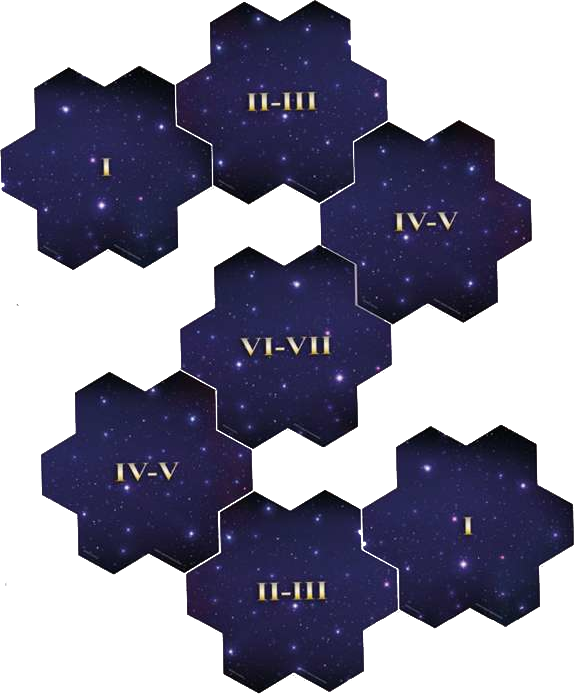
\includegraphics[width=\columnwidth, keepaspectratio]{\maps/the-hunt-2.png}

\medskip

{\footnotesize\centering\textbf{\MakeUppercase{2-PLAYER SCENARIO}}\par}

\begin{tikzpicture}[overlay, anchor=north]
  \centering
  \node at (0, 0) {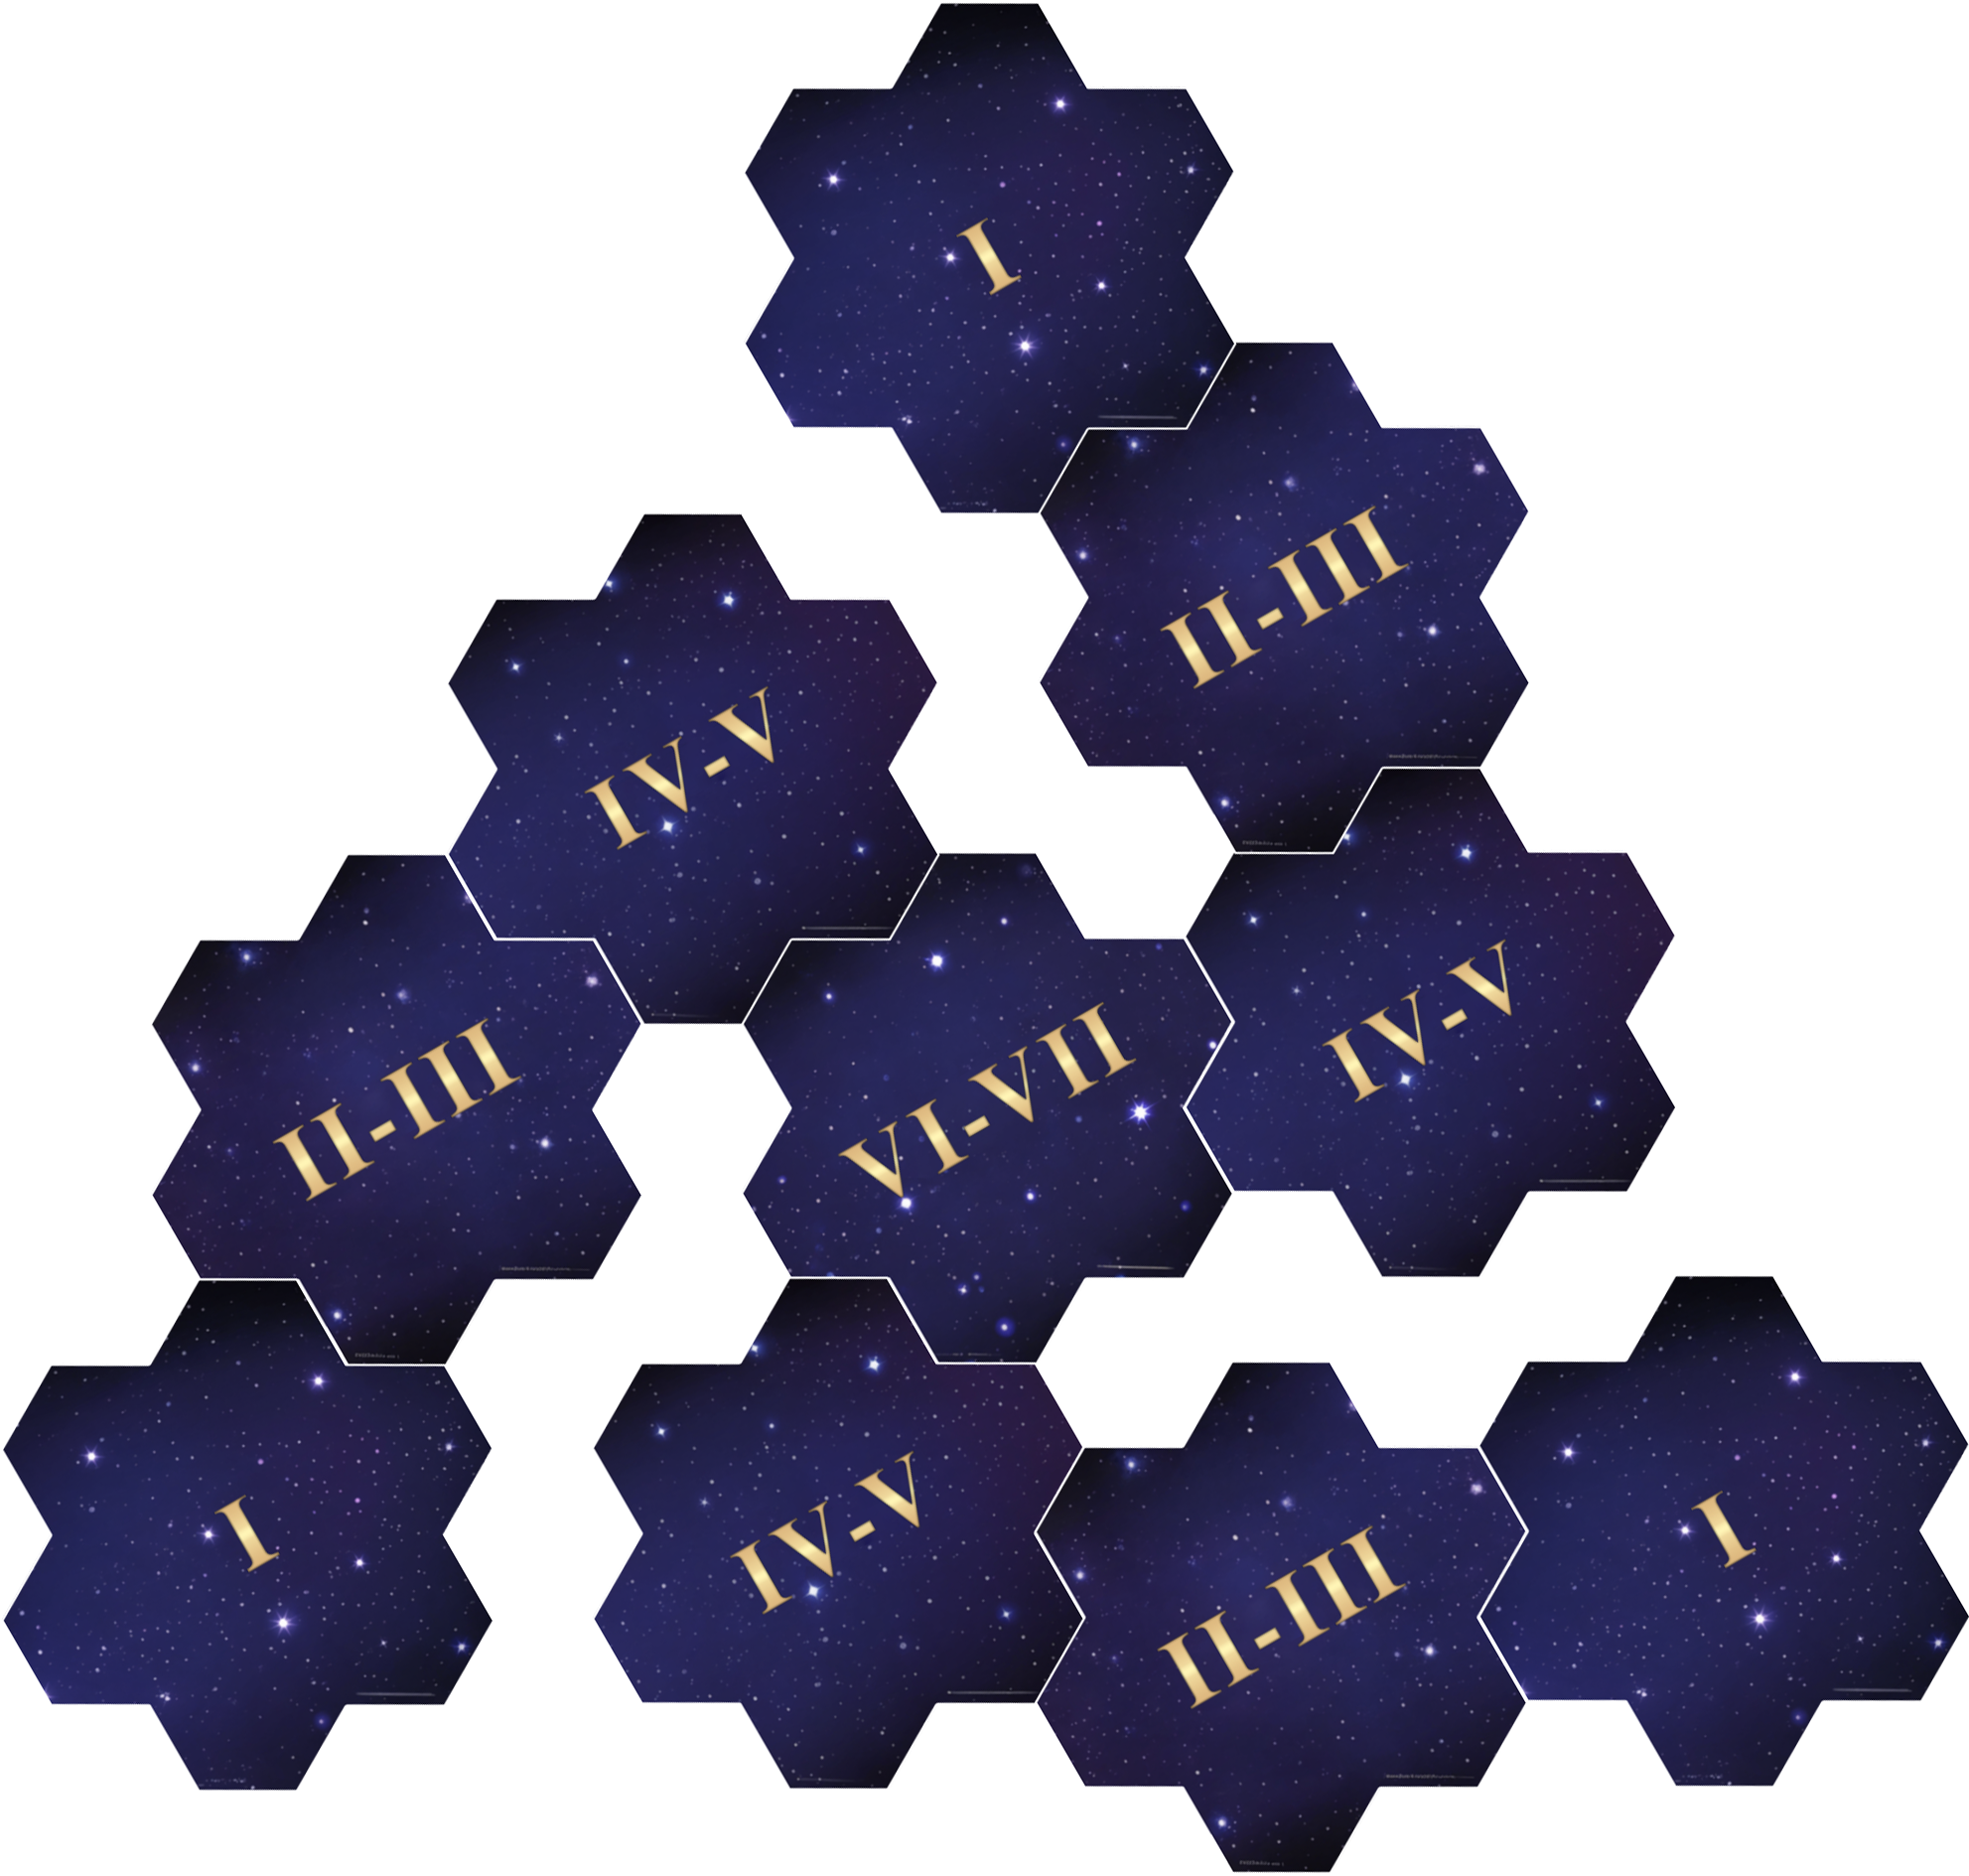
\includegraphics[width=\textwidth, height=0.48\textheight, keepaspectratio]{\maps/the-hunt-3.png}};
  \node at (0, -12) {\footnotesize{\textbf{\MakeUppercase{3-PLAYER SCENARIO}}}};
\end{tikzpicture}

\end{multicols*}

\clearpage

\begin{wrapfigure}{l}{0.3\textwidth}
  \raisebox{0pt}[\dimexpr\height-0.2\baselineskip\relax]{\framedimage[1.1\linewidth]{\art/azure_dragon.jpg}}
\end{wrapfigure}
{
  \textbf{\MakeUppercase{Boss: Azure Dragon}}

  \medskip

  \textit{Little is known of the Azure Dragon.
    It is both rare and mighty, thus few have seen it, and fewer still have survived its attacks.
    This powerful creature is not much bigger than most dragons, but is said to be capable of enduring prolonged physical attack.
    It is said those standing face-to-face with an Azure Dragon tend to freeze from pure fear.
  }

  \medskip

  \textbf{Fighting the Azure Dragon:}
  \begin{enumerate}
    \item Place the Azure Dragon Miniature/Card on the battlefield.
      Ignore its ability.
    \item Prepare a pile of discarded Artifacts and shuffle it.
  \end{enumerate}

  \medskip

  \textbf{Rules:}
  \begin{itemize}
    \item \textit{Hoarding Tendency:} At the start of each Turn, randomly choose a Card from the shuffled pile of discarded Artifacts.
      If the Artifact is:
      \begin{itemize}
        \item A weapon: The Dragon gains one Breath attack that targets three creatures in a row.
          The Unit directly hit in the middle suffers full damage, while the Units on both sides suffer 3\,\svg{damage} less.
        \item A piece of armor, shield, or clothing: The Dragon gains 3\,\svg{defense}, represented with spare Faction Cubes.
          Remove them after they have absorbed damage.
        \item A trinket: The Azure Dragon roars and summons an ice storm, causing all creatures to freeze in fear.
          This results in every Unit moving only 1 Field per Round, while the Azure Dragon can fly to any Field on the Combat Board.
      \end{itemize}
    \item The Azure Dragon is immune to all Spells cast against it.
    \item Buffs and enhancements cast on player's Units remain effective.
  \end{itemize}
}

\bigskip

\hommtable[]{8}{
  \centering
  \medskip

  \let\origbronze\bronze
  \let\origsilver\silver
  \let\origgolden\golden
  \let\origazure\azure
  \renewcommand{\bronze}{\origbronze[20]}
  \renewcommand{\silver}{\origsilver[20]}
  \renewcommand{\golden}{\origgolden[20]}
  \renewcommand{\azure}{\origazure[20]}

  \begin{tabularx}{0.95\linewidth}{XXXX}
  \darkcell{\raisebox{-.2\height}{\bronze} \textbf{Easy}} &
  \darkcell{\raisebox{-.2\height}{\silver} \textbf{Normal}} &
  \darkcell{\raisebox{-.2\height}{\golden} \textbf{Hard}} &
  \darkcell{\raisebox{-.2\height}{\azure} \textbf{Impossible}}\\
  \lightcell[1.8]{No additional\\changes} &
  \lightcell[1.8]{\raisebox{-.25\height}{
\includegraphics[height=15px]{\images/hp.png}} 22} &
  \lightcell[1.8]{\raisebox{-.25\height}{
\includegraphics[height=15px]{\images/hp.png}} 30} &
  \lightcell[1.8]{\raisebox{-.25\height}{
\includegraphics[height=15px]{\images/hp.png}} 40 \\ +2 \svg{attack-yellow} \\ +2 \svg{defense-yellow}}
  \end{tabularx}
}

\clearpage

\begin{wrapfigure}{l}{0.3\textwidth}
  \raisebox{0pt}[\dimexpr\height-0.2\baselineskip\relax]{\framedimage[1.1\linewidth]{\art/crystal_dragon.jpg}}
\end{wrapfigure}
{
  \textbf{\MakeUppercase{Boss: Crystal Dragon}}

  \medskip

  \textit{Made entirely from red crystal and brought to life through magical means, the Crystal Dragon is literally semitransparent, lit from the center by its magical heart.
    Used frequently as a training tool for young dragon slayers, many wizards also create these creatures for the crystal they shed.
  }

  \medskip

  \textbf{Fighting the Crystal Dragon:}
  \begin{enumerate}
    \item Place the Crystal Dragon Miniature/Card on the battlefield.
      Ignore its ability.
    \item Place two Gold Golems and two Diamond Golems on the battlefield.
  \end{enumerate}

  \medskip

  \textbf{Rules:}
  \begin{itemize}
    \item At the start of every battle Round, check if any of the Golems were removed in the previous Round.
      If so, spawn one new Diamond or Gold Golem (chosen randomly) in the last row of the battlefield.
    \item \textit{Golem Devour:} The Crystal Dragon can consume Golems to regain health.
      During its Turn, if the Crystal Dragon is adjacent to a Golem, it can choose to consume it, removing a certain amount of \svg{damage} based on the type of Golem consumed:
      \begin{itemize}
        \item Consuming a Gold Golem: Remove 2 \svg{damage}.
        \item Consuming a Diamond Golem: Remove 4 \svg{damage}.
        \item[] \textbf{Note:} The Crystal Dragon can only consume one Golem per Turn.
      \end{itemize}
    \item Golem Abilities: Gold and Diamond Golems do not possess any additional abilities beyond those specified on their Cards.
      They primarily serve as fodder for the Crystal Dragon's health regeneration.
    \item The Crystal Dragon \textit{retaliates twice} per battle Round.
  \end{itemize}
}

\bigskip

\hommtable[]{10}{
  \centering
  \medskip

  \let\origbronze\bronze
  \let\origsilver\silver
  \let\origgolden\golden
  \let\origazure\azure
  \renewcommand{\bronze}{\origbronze[20]}
  \renewcommand{\silver}{\origsilver[20]}
  \renewcommand{\golden}{\origgolden[20]}
  \renewcommand{\azure}{\origazure[20]}

  \begin{tabularx}{0.95\linewidth}{XXXX}
  \darkcell{\raisebox{-.2\height}{\bronze} \textbf{Easy}} &
  \darkcell{\raisebox{-.2\height}{\silver} \textbf{Normal}} &
  \darkcell{\raisebox{-.2\height}{\golden} \textbf{Hard}} &
  \darkcell{\raisebox{-.2\height}{\azure} \textbf{Impossible}}\\
  \lightcell[2.8]{No additional\\changes} &
  \lightcell[2.8]{\raisebox{-.25\height}{
\includegraphics[height=15px]{\images/hp.png}} 22} &
  \lightcell[2.8]{{\raisebox{-.25\height}{
\includegraphics[height=15px]{\images/hp.png}} 26 \\ +1 Retaliation}} &
  \lightcell[2.8]{\raisebox{-.25\height}{
\includegraphics[height=15px]{\images/hp.png}} 32 \\ +1 Retaliation  \\ Remove additional 2 \svg{damage-yellow} by consuming Golems} \\
  \end{tabularx}
}

\vspace{-1em}

\begin{wrapfigure}{l}{0.3\textwidth}
  \raisebox{0pt}[\dimexpr\height-1.2\baselineskip\relax]{\framedimage[1.1\linewidth]{\art/rust_dragon.jpg}}
\end{wrapfigure}
{
  \textbf{\MakeUppercase{Boss: Rust Dragon {\scriptsize Requires Fortress Expansion}}}

  \medskip

  \textit{Rust Dragons are known to hunt Gorgons, and live and feed in sulfur mines.
    With this appetite, Rust Dragons spew a concentrated acid as their primary attack.
    This acid is capable of eating through the strongest armor, lowering the defense of its target while inflicting further damage.
  }

  \medskip

  \textbf{Fighting the Rust Dragon:}
  \begin{enumerate}
    \item Place the Rust Dragon Miniature/Card on the battlefield.
      Ignore its ability.
    \item Prepare four spare M\&M Deck Cards to mark pools of acid.
  \end{enumerate}

  \medskip

  \textbf{Rules:}
  \begin{itemize}
    \item The Rust Dragon is immune to basic Spells.
    \item \textit{Corrosive Vomit:} The Rust Dragon has a powerful crowd control ability that allows it to spew four pools of sulfuric acid onto the battlefield \textit{at the beginning} of each Combat Round.
      Use M\&M Deck Cards placed face down to mark their locations.
    \item The Rust Dragon cannot place pools on the same Fields as in the previous Round.
      Mark the Fields with spare Faction Cubes to indicate where the pools were located.
    \item The pools of sulfuric acid block battlefield Fields and impede movement for one Round only.
      They serve as Obstacles for both players and the Dragon.
    \item The Rust Dragon's passive ability, \textit{Corrosion}, decreases an enemy Unit's armor by 2 with each attack.
      Place a spare Faction Cube on the Unit's Card to indicate this effect.
      Corrosion stacks up to -4 \svg{defense}.
  \end{itemize}
}

\vspace{5em}

\hommtable[]{9}{
  \centering
  \medskip

  \let\origbronze\bronze
  \let\origsilver\silver
  \let\origgolden\golden
  \let\origazure\azure
  \renewcommand{\bronze}{\origbronze[20]}
  \renewcommand{\silver}{\origsilver[20]}
  \renewcommand{\golden}{\origgolden[20]}
  \renewcommand{\azure}{\origazure[20]}

  \begin{tabularx}{0.95\linewidth}{XXXX}
  \darkcell{\raisebox{-.2\height}{\bronze} \textbf{Easy}} &
  \darkcell{\raisebox{-.2\height}{\silver} \textbf{Normal}} &
  \darkcell{\raisebox{-.2\height}{\golden} \textbf{Hard}} &
  \darkcell{\raisebox{-.2\height}{\azure} \textbf{Impossible}}\\
  \lightcell[2.5]{No additional\\changes} &
  \lightcell[2.5]{\raisebox{-.25\height}{
\includegraphics[height=15px]{\images/hp.png}} 20} &
  \lightcell[2.5]{\raisebox{-.25\height}{
\includegraphics[height=15px]{\images/hp.png}} 32} &
  \lightcell[2.5]{\raisebox{-.25\height}{
\includegraphics[height=15px]{\images/hp.png}} 40 \\ +1 to Corrosion armor decrease} \\
  \end{tabularx}
}

\vspace{-1em}

\begin{wrapfigure}{l}{0.28\textwidth}
  \raisebox{0pt}[\dimexpr\height-0.2\baselineskip\relax]{\framedimage[1.1\linewidth]{\art/faerie_dragon.jpg}}
\end{wrapfigure}
{
  \textbf{\MakeUppercase{Boss: Faerie Dragon {\scriptsize Requires Rampart Expansion}}}

  \medskip

  \textit{Faerie Dragons are deceptively cute, but in truth, are mischievous tricksters.
    Little is known about these notorious troublemakers.
    What is known is found more in storybooks than magical tomes.
    Some say they are invisible.
    Some say they can cast spells.
    Some say Magic Mirror is one of their natural defensive traits.
  }

  \medskip

  \textbf{Fighting the Faerie Dragon:}
  \begin{enumerate}
    \item Place 2 Faerie Dragon Cards on the battlefield.
      Ignore their abilities.
    \item Place 1 Dendroid Card from the \svg{silver} Neutral Units Deck onto the battlefield, and place 3 additional Cards face down to represent the other 3 Dendroids.
  \end{enumerate}

  \medskip

  \textbf{Rules:}
  \begin{itemize}
    \item The Faerie Dragon is immune to basic Spells.
    \item The Faerie Dragon can cast up to two different Spells per battle Round.
    \item All Spells are displayed visibly next to the Combat Board:
      \begin{enumerate}
        \item The first Spell is \textit{Lightning}.
        \item The second Spell is \textit{Cure}.
        \item For the third Spell, the Faerie Dragon randomly picks an expert Spell from the Spell Deck, excluding Map \svg{map} Spells.
          If a Map \svg{map} Spell is picked, draw another Spell.
      \end{enumerate}
    \item \textit{Trickster:} In the first Round of the battle, the first targeted Faerie Dragon is a mere mirage.
      It inflicts damage, but disappears from the battlefield when hit by an enemy.
    \item Dendroids' Ability: Each Dendroid holds a key to the Faerie Dragon's power.
      After the second Dendroid dies, start removing one Spell from the Faerie Dragon's spellbook, beginning with the third Spell.
      Decrease the dragon's Spell Empowerment \svg{empower} by one (starting from its maximum) upon vanquishing the 2nd, 3rd, and 4th Dendroids.
      When there are no Dendroids left, the dragon loses the ability to cast Spells.
  \end{itemize}
}

\bigskip

\hommtable[]{7}{
  \centering
  \medskip

  \let\origbronze\bronze
  \let\origsilver\silver
  \let\origgolden\golden
  \let\origazure\azure
  \renewcommand{\bronze}{\origbronze[20]}
  \renewcommand{\silver}{\origsilver[20]}
  \renewcommand{\golden}{\origgolden[20]}
  \renewcommand{\azure}{\origazure[20]}

  \begin{tabularx}{0.95\linewidth}{XXXX}
  \darkcell{\raisebox{-.2\height}{\bronze} \textbf{Easy}} &
  \darkcell{\raisebox{-.2\height}{\silver} \textbf{Normal}} &
  \darkcell{\raisebox{-.2\height}{\golden} \textbf{Hard}} &
  \darkcell{\raisebox{-.2\height}{\azure} \textbf{Impossible}}\\
  \lightcell[1.6]{No additional\\changes} &
  \lightcell[1.6]{\raisebox{-.25\height}{
\includegraphics[height=15px]{\images/hp.png}} 18} &
  \lightcell[1.6]{\raisebox{-.25\height}{\includegraphics[height=15px]{\images/hp.png}} 26} &
  \lightcell[1.6]{\raisebox{-.25\height}{\includegraphics[height=15px]{\images/hp.png}} 32 \\ +1 Mirage} \\
  \end{tabularx}
}



\addscenariogroup{\campaignstitle}{\layout/campaigns.png}

\clearpage

% !TeX spellcheck = en_US
\addscenariosection{1}{Inferno Campaign -- Dungeons and Devils}{1. A Devilish Plan}{\images/inferno.png}

\begin{multicols*}{2}

\textbf{Author:} Tm335

\textbf{Source:} \href{https://discord.com/channels/740870068178649108/1243057664666238996/1243057664666238996}{Archon Studios Discord}

\textit{A large elvish population inhabits Erathia's southeastern coast.
  Green and gold dragons, native to the region, augment their military strength.
  Before we conquer this region and redirect our forces to Steadwick, we must annihilate these dragons.
  Our Kreegan allies from Eeofol have requested the honor of this mission.
  The Kreegans are fierce warriors; they will relish the slaughter.}

\subsection*{\MakeUppercase{Scenario length}}

This scenario plays out over 13 rounds.

\subsection*{\MakeUppercase{Player setup}}

\textbf{Faction:} Inferno

\textbf{Faction Hero:} Choose any   

\textbf{Starting Resources:}\par
\resources{15}{3}{1}

\textbf{Starting Income:}\par
\resources{10}{0}{0}

\textbf{Starting Units:}

\begin{itemize}
  \item A Pack of Familiars
  \item A Few Magogs
\end{itemize}

\textbf{Town Buildings:} \svg{bronze} Dwelling, City Hall

\vspace*{\fill}\columnbreak

\textbf{Bonus:} Choose one of the following options: 
\begin{itemize}
  \item Add a ``Slayer'' spell to your hand
  \item Add the ``Armor of Wonder'' Artifact to your hand
  \item Reinforce Magogs and gain 1 \svg{valuables}
\end{itemize}

\subsection*{\MakeUppercase{AI hero setup}}

\textbf{Faction:} Rampart

\textbf{Enemy Armies:} 

\begin{itemize}
  \item \textbf{Gold Dragon Army:} A Pack of Gold Dragons, a Pack of Unicorns, a Pack of Dendroids, a Pack of Centaurs
  \item \textbf{Ivor's Army:} A Few Elves\footnote{In Round 9, the Few Elves in Ivor's Army are reinforced to a Pack of Elves.}, Neutral Army at the same level as your Hero level\footnote{See page 35, ``Field Difficulty Level Table'' in the Core Rulebook, for further details on the number of Neutral Units you have to draw for this Neutral Army.}
\end{itemize}

\textbf{Ivor's Deck:} 1 × Might card, 2 × Magic card, 1 × Skill card

\textbf{Ivor's Spell Deck:} 1 × Precision Spell card (it resolves on the first ranged unit able to make a ranged attack), 1 × Magic Arrow Spell card

\textbf{Ivor's Skill:} Archery Ability card (it always resolves its Basic effect)

\subsection*{\MakeUppercase{Map setup}}

Take the following Map tiles and set them up as shown in the scenario map layout:

\textbf{2 × Starting Map tile (I)}
\begin{itemize}
  \item 1 × Inferno (S6)
  \item 1 × Rampart (S4)
\end{itemize}

\vspace*{\fill}\columnbreak

\textbf{3 × Far Map tile (II-III)}
\begin{itemize}
  \item \mbox{2 × Inferno (choose from: F16-F18, \#F10)}
  \item 1 × Rampart (choose from: F10-F12)
\end{itemize}

\textbf{2 × Near Map tile (IV-V)}
\begin{itemize}
  \item 2 × Rampart (N7, N8)
\end{itemize}

\textbf{1 × Center Map tile (VI-VII)}
\begin{itemize}
  \item 1 × Dragon Utopia Center Map tile (C1)
\end{itemize}

\subsection*{\MakeUppercase{Heroes placement}}

The Enemy Hero is represented by one Rampart faction Hero model of your choice
and appears in the center field of the S4 Starting Map tile.

Place your Hero in the center field of the Inferno Starting Map tile.

\subsection*{\MakeUppercase{Victory Conditions}}

Defeat the Enemy Hero and the Gold Dragons Armies.

\subsection*{\MakeUppercase{Defeat Conditions}}

You lose one Combat encounter.

You fail to defeat the Enemy Hero and the Gold Dragon Armies by the end of the Round 13.

\subsection*{\MakeUppercase{Timed Events}}

\textbf{1$^{st}$ Round:}
\begin{itemize}
  \item Read: ``Our underlings have done well. They have managed to raise a volcano
    and erect a fort in a sparsely populated forest just outside of Erathia's border.
    While the Dungeon Overlords make their way underground toward the Erathian capitol,
    you must strike at their allies, the elves of AvLee.'
\end{itemize}

\textbf{2$^{nd}$ Round:}
\begin{itemize}
  \item Read: ``The Gold Dragon Queen is a powerful ally of AvLee.
    You must find her lair and see to her demise, as this will greatly weaken
    the elves and make them less of a threat to our plans to destroy Erathia.
    Go now, and make us proud!''
\end{itemize}

\textbf{9$^{th}$ Round:}
\begin{itemize}
  \item The Few Elves of Ivor's Army are Reinforced to a Pack of Elves.
    Ivor's Army also gains an Ammo Cart.
\end{itemize}

\textbf{10$^{th}$ Round:}
\begin{itemize}
  \item The Rampart Faction Town that Ivor's Army resides in gains an Arrow Tower.
\end{itemize}

\textbf{13$^{th}$ Round:}
\begin{itemize}
  \item At the end of the round, if both the Enemy Hero and the Gold Dragon Armies are not defeated, all is lost - you lose!
\end{itemize}

\textbf{When you complete the scenario:}
\begin{itemize}
  \item Read: ``Congratulations! You have completed your quest to kill the fearsome beast, and can claim victory!'
\end{itemize}


\subsection*{\MakeUppercase{Additional rules}}

During this ``Inferno'' campaign scenario, the following rules apply:

\begin{itemize}
    \item Your Hero does not gain Experience past Level 5.
    \item The Enemy Hero does not move and only waits in their Town. They start with Walls and a Gate on their side of the Combat Board.
    \item The N7 Map tile cannot be entered until Ivor is defeated.
    \item At the Dragon Utopia location, your Hero fights the Gold Dragons Army.
    \item The ``Castle Gate'' cannot be built.
    \item If your Hero visits an Obelisk, you may Search (2) the Ability deck, the Artifact deck, or the Spell deck.
\end{itemize}

\end{multicols*}

\begin{figure*}[!hb]
  \newcommand{\maplabel}[1]{}
  \centering
  \includegraphics[width=0.8\textwidth]{\_assets/maps/inferno_devilish_plan.png}
  \begin{tikzpicture}[overlay]
    \node at (-13, 9.2) {\large{{\textbf{\textcolor{darkcandyapplered}{N8}}}}};
    \node at (-4, 9.3) {\large{{\textbf{\textcolor{darkcandyapplered}{N7}}}}};
    \node at (-11.3, 0.2) {\large{{\textbf{\textcolor{darkcandyapplered}{Inferno Map}}}}};
    \node at (-11.3, -0.5) {\large{{\textbf{\textcolor{darkcandyapplered}{Tiles}}}}};
  \end{tikzpicture}
\end{figure*}


\clearpage

% !TeX spellcheck = en_US
\addscenariosection[subsection]{1}{Inferno Campaign $-$ Dungeons and Devils}{2. Steadwick's Fall}{\images/firewall.png}

\begin{multicols*}{2}

\textbf{Author:} Tm335

\textbf{Source:} \href{https://discord.com/channels/740870068178649108/1246353361456861276/1246353361456861276}{Archon Studios Discord}

\textit{Catherine Ironfist has enlisted aid from Bracada and AvLee.
She knows we are close to Steadwick.
We must occupy Steadwick before she arrives.
Once we own Erathia's capitol, not even Catherine Ironfist will wrench it from our hands.}

\subsection*{\MakeUppercase{Scenario Length}}

This Scenario plays out over 16 Rounds.

\subsection*{\MakeUppercase{Player Setup}}

\textbf{Faction:} Inferno

\textbf{Faction Hero:} Choose any

\textbf{Starting Resources:} 15 \svg{gold}, 1 \svg{building_materials}, 1 \svg{valuables}

\textbf{Starting Income:} 10 \svg{gold}, 2 \svg{building_materials}, 0 \svg{valuables}

\textbf{Starting Units:}

\begin{itemize}
  \item A Few Troglodytes
  \item A Few Evil Eyes
  \item A Pack of Familiars
\end{itemize}

\textbf{Town Buildings:} \svgunit{bronze} Dwelling, \svgunit{silver} Dwelling

\textbf{Bonus:} Choose one of the following options:
\begin{itemize}
  \item Add a Pack of Harpies to your hand.
  \item Add a Pack of Magogs to your hand.
  \item Add an Ammo Cart to your hand.
  \item Search (4) the Spell Deck.
\end{itemize}

\subsection*{\MakeUppercase{AI Hero Setup}}

\textbf{General Kendal (Castle):}
\begin{itemize}
    \item \textbf{Army:}
    \begin{itemize}
        \item A Pack of Archangels
        \item A Pack of Champions
        \item A Pack of Zealots
        \item A Pack of Crusaders
        \item A Pack of Griffins
        \item A Balista War Machine
    \end{itemize}
    \item \textbf{AI Deck:}
    \begin{itemize}
        \item 5 × Might \svg{might} Card
        \item 1 × Magic \svg{magic} Card
        \item 3 × Skill \svg{skill} Card
    \end{itemize}
    \item \textbf{Spells:}
    \begin{itemize}
        \item 2 × Haste
    \end{itemize}
    \item \textbf{Abilities:}
    \begin{itemize}
        \item Artillery\footnote{For General Kendal, the Artillery Ability Card always resolves the Expert effect and the Ballista War Machine Activates every time the Artillery Ability Card is drawn, as well as at the beginning of a Combat Round.}
    \end{itemize}
\end{itemize}

\textbf{Charging Heroes (Rampart, Tower, Castle):}
\begin{itemize}
    \item \textbf{Army:}
       Neutral Army one Level higher than your Hero Level (Max Level VI)\footnote{See page 35, ``Field Difficulty Level Table'' in the Core Rulebook, for further details on the number of Neutral Units you have to draw for this Neutral Army.}
    \item \textbf{AI Deck:}
    \begin{itemize}
        \item 2 × \svg{might} Might Card
        \item 2 × \svg{magic} Magic Card
    \end{itemize}
    \item \textbf{Spells:}
    \begin{itemize}
        \item 2 × Slow\footnote{All the Charging Heroes' Enemies use the same AI and Spell Decks. Reset them after every Combat.}
    \end{itemize}
\end{itemize}

\subsection*{\MakeUppercase{Map Setup}}

Take the following Map Tiles and set them up as shown in the Scenario map layout:

\textbf{2 × Starting (I) Map Tile}
\begin{itemize}
  \item 1 × Inferno (S6)
  \item 1 × Castle (S3)
\end{itemize}

\textbf{3 × Far (II--III) Map Tile}
\begin{itemize}
  \item 1 × Castle (F3)
  \item 1 × Rampart (F10)
  \item 1 × Dungeon (F2)
  \item 1 × Tower (\#F1)
  \item 1 × Rampart (choose from: F11, F12)
  \item 1 × Necropolis (choose from: F4, \#F6, F7)
\end{itemize}

\textbf{2 × Near (IV--V) Map Tile}
\begin{itemize}
  \item 2 × Castle (N3, choose from: \#N3, N6)
  \item 1 × Rampart (N8)
  \item 1 × Necropolis (N4)
\end{itemize}

\subsection*{\MakeUppercase{Heroes Placement}}

The Enemy Hero General Kendal is represented by a Castle Faction Hero model and appears on the center Field of the S3 Starting Map Tile.

The Castle Charging Hero is represented by a Castle Faction Hero model and appears on (and owns) the Settlement of the F3 Map Tile.

The Rampart Charging Hero is represented by a Rampart Faction Hero model and appears on (and owns) the Settlement of the F10 Map Tile.

The Tower Charging Hero is represented by one Tower Faction Hero model and appears on (and owns) the Settlement of the \#F1 Map Tile.

Place your Main Hero on the center Field of the Inferno Starting S6 Map Tile.

Place your Secondary Hero, represented by one Dungeon Faction Hero model of your choice, on the Settlement of the F2 Map Tile. This Settlement produces no resources.

\subsection*{\MakeUppercase{Victory Conditions}}

Capture all Enemy Settlements (F3, F10, \#F1) and Steadwick (S3) before Queen Catherine Ironfist arrives at the end of Round 16.

\subsection*{\MakeUppercase{Defeat Conditions}}

You lose if any of the following occur:
\begin{itemize}
  \item You lose one Combat encounter with your Main Hero (Surrendering costs 10 \svg{gold}, and does not count as a defeat).
  \item You lose your Faction Town on the S6 Map Tile.
  \item You run out of time -- you have time till the end of Round 16.
\end{itemize}

\subsection*{\MakeUppercase{Timed Events}}

\textbf{\nth{1} Round:}
\begin{itemize}
  \item Read ``Congratulations'' section.
\end{itemize}

\textbf{\nth{2} Round:}
\begin{itemize}
  \item Read ``News'' section.
\end{itemize}

\textbf{\nth{5} Round:}
\begin{itemize}
  \item Read: ``First Report'' section.
\end{itemize}

\textbf{\nth{10} Round:}
\begin{itemize}
  \item For any Enemy Settlements (F3, F10, \#F1) that have not been defeated, an additional Enemy
    Charging Hero of that Faction appears on each Settlement at the beginning of this Round.
\end{itemize}

\textbf{\nth{11} Round:}
\begin{itemize}
  \item Read ``Second Report'' section.
\end{itemize}

\textbf{\nth{13} Round:}
\begin{itemize}
  \item Read ``First Warning'' section.
\end{itemize}

\textbf{\nth{15} Round:}
\begin{itemize}
  \item Read ``Second Warning'' section.
\end{itemize}

\textbf{\nth{16} Round:}
\begin{itemize}
  \item Read ``The Ending'' section \textbf{at the end of the Round}.
\end{itemize}

\textbf{When you complete the Scenario:}
\begin{itemize}
  \item Read: ``Congratulations! You captured Steadwick and are victorious!''
\end{itemize}

\subsection*{\MakeUppercase{Additional Rules}}

During this ``Inferno'' Campaign Scenario, the following rules apply:

\begin{itemize}
    \item General Kendal does not move and only waits in his Town. He start with Walls, Gate,
      and Arrow Tower on his side of the Combat Board.
    \item The difficulty Level of every Combat encounter on the map increases by one till the end of the Scenario
      (see page 35, ``Field Difficulty Level Table'' in the Core Rulebook).
    \item The Enemy Charging Heroes have only 2 Movement Points, instead of 3. They ignore everything else
      (including Mines and Settlements if possible) and go straight for the player's Faction Town (on Map Tile S6).
      They do not pursue the player directly, but if they happen to be on the same Map Tile, they will
      attack the player's Main Hero (not Secondary).
    \item The borders on the Castle Starting Map Tile S3 cannot be crossed by any means until
      all Enemy Settlements (F3, F10, \#F1) have been defeated.
    \item Gain 2 \svg{valuables} every time you defeat Enemy Charging Heroes.
    \item Obelisks give you 1 \svg{valuables} and function as a ``Castle Gate'' location (only if you have the ``Castle Gate'' built in your Town).
\end{itemize}

\subsection*{\MakeUppercase{The Story}}

\textbf{Congratulations}

You are to be congratulated on your progress so far.
You have laid waste to Eastern Erathia, and are now within striking distance of the Erathian capital of Steadwick.
You must capture the capital quickly!

\textbf{News}

Not only have Bracada and AvLee sent reinforcements, but we have received news that Queen Catherine Ironfist is marching a sizeable army from the south.
We must control the capital and its garrisons before she arrives.

You have just received a report on the progress of Queen Catherine.
Forces from Nighon and Eeofol are attempting to delay her march to Steadwick, but doubt that they can delay her more than two or three months.

\textbf{First Report}

You receive a report from the south.
Queen Catherine's forces have been sufficiently delayed, allowing you at least two months more to reach the capitol, but our own forces have suffered significant losses.
Do not let their sacrifice go to waste.

\textbf{Second Report}

You receive a report from the south.
Our forces continue to throw themselves in the path of Queen Catherine's armies, yet she continues to march northward.
You have, at most, three or four weeks before she can reach the capital.

\textbf{First Warning}

Queen Catherine's march continues -- her forces are just two weeks away.
If you do not hurry, we will not have time to secure the capital before her arrival.

\textbf{Second Warning}

Your scouts report sighting Queen Catherine's army seven days to the southwest.
If she reaches the capitol before you, all is lost.

\textbf{The Ending}

This morning, a massive army lead by Queen Catherine Ironfist arrived at the Erathian capitol of Steadwick.
We have no choice but to retreat our forces.
You have failed us... miserably.

\textcolor{darkcandyapplered}{If Steadwick has not been captured, the Scenario is lost!}

\end{multicols*}

\begin{tikzpicture}[remember picture, overlay]
  \node(bg)[anchor=center, yshift=37em, opacity=0.17] at (current page.south) {
    \includegraphics[width=0.85\paperwidth, keepaspectratio]{\art/fire_shield.png}
  };
  \node(map)[anchor=center] at (current page.center) {
    \includegraphics[width=\textwidth]{\maps/inferno_steadwicks_fall.png}
  };

  \node at (3, -11.5) {\large{{\textbf{\textcolor{darkcandyapplered}{N3}}}}};
  \node at (4.4, -18.6) {\large{{\textbf{\textcolor{darkcandyapplered}{\#F1}}}}};
  \node at (15, -5.2) {\large{{\textbf{\textcolor{darkcandyapplered}{F10}}}}};
  \node at (17.3, -11.5) {\large{{\textbf{\textcolor{darkcandyapplered}{S6}}}}};
  \node at (8.8, -18.8) {\large{{\textbf{\textcolor{darkcandyapplered}{F3}}}}};
  \node at (15.9, -18.8) {\large{{\textbf{\textcolor{darkcandyapplered}{F2}}}}};
  \node at (2, -4.5) {\large{{\textbf{\textcolor{darkcandyapplered}{Steadwick}}}}};
  \node at (2, -5.2) {\large{{\textbf{\textcolor{darkcandyapplered}{S3}}}}};
  \node at (7.5, -5.4) {\large{{\textbf{\textcolor{darkcandyapplered}{Rampart}}}}};
  \node at (7.5, -6.1) {\large{{\textbf{\textcolor{darkcandyapplered}{Map Tiles}}}}};
  \node at (12.4, -17.8) {\large{{\textbf{\textcolor{darkcandyapplered}{Necropolis}}}}};
  \node at (12.4, -18.5) {\large{{\textbf{\textcolor{darkcandyapplered}{Map Tiles}}}}};
  \node at (2, -12.3) {\large{{\textbf{\textcolor{darkcandyapplered}{Castle}}}}};
  \node at (2, -13) {\large{{\textbf{\textcolor{darkcandyapplered}{Map Tiles}}}}};
\end{tikzpicture}


% !TeX spellcheck = en_US
\addsection{Recommendations}{\art/haste.png}

\iftoggle{printable}{}{\bigbreak}

\begin{multicols*}{2}
We've compiled some custom rules and best practices to enhance your gaming experience.
Keep in mind that these are just the \textbf{opinions of the authors} of this book.
Enjoy!

\subsection*{Play Time}

You can estimate your \textbf{minimal} play time using the following formula:

\begin{center}
  Play Time $= \boldsymbol{P × R × 5}$ [min]
\end{center}

Where:
\begin{itemize}
  \item[$\textbf{P}$] -- number of players
  \item[$\textbf{R}$] -- number of Rounds
\end{itemize}

For example, if you're playing a 3-player Scenario consisting of 12 Rounds, you can easily calculate that $3 \times 12 \times 5 = 180$.
Your expected minimal play time would be around 3 hours.

To calculate the \textbf{upper bound} of your play time (more realistic if there are inexperienced players), simply double the result.
In this case, that would be 6 hours.

\subsection*{Magic Arrows}

Except for the Magic Arrow, each Spell appears exactly twice in the Spell Deck.
After players prepare their starting M\&M Decks, it is recommended to remove Magic Arrows from the Spell Deck until no more than two remain.

\subsection*{Guaranteed Settlement}

When distributing Far Tiles (II--III) between players, each player's pool of Map Tiles must include one Settlement.

\includegraphics[width=\linewidth]{\art/rogue.jpg}

\includegraphics[width=\linewidth]{\art/medusa.jpg}

\subsection*{War Machines as Artifacts}

Shuffle one of each War Machine into the Artifact Deck before the start of the game.
If using the optional Tournament rule of splitting the Artifact Deck, shuffle the War Machines into the Major Artifact Deck.

\subsection*{Round One Mulligan}

At the start of the \nth{1} Round, each player may reshuffle their hand of Cards back into their Deck of Might and Magic and draw a new starting hand of Cards once.

\subsection*{Tier V--VII Combat on Hard+ Difficulty}

Treat Level V--VII Combats as one difficulty step lower when playing on Hard or Impossible.
For example, a Level VII Combat on Hard will be against 2 × \svgunit{azure} Neutral Units.

\subsection*{Trading Post}

Although rules as written state that you can remove only one card from your hand while Visiting a Trading Post, it is recommended to allow removing as many as you like.

\subsection*{Victory Points}

When playing with the optional Victory Points from the Tournament book, the following rules apply (unless overruled by the Scenario):
\begin{itemize}
  \item Faction Towns grant 1 VP.
  \item Possessing the Grail at the end of the match grants 3 VPs. If the Grail was transported to that player's Faction Town, it grants 5 VPs instead.
  \item Capturing a Dragon Utopia grants 3 VPs.
\end{itemize}

\end{multicols*}

\begin{multicols}{2}

\subsection*{Combat with Neutral Units}

During Combat with Neutral Units in clash Scenarios, if a player decides to deploy their Units only on one half (left or right) of the battle Board, the player positioning the Neutral Units must do the same.

Placing Neutral Units far apart only makes the other player waste MPs, which slows the game down.
The exception to this rule is when there are three Neutral \svg{unit_ground} or \svg{unit_flying} Units to position, as all of them must go to the front line.
See examples that follow.

\begin{center}
  \includegraphics[width=0.65\linewidth]{\art/resurrection.png}
\end{center}

\end{multicols}

\begin{figure*}[!h]
  \mbox{}
  \hfill
  \begin{minipage}[t]{0.44\textwidth}
    \centering
    \includegraphics[width=\linewidth]{\examples/battle_good.png}
    \caption[good protected]{\textit{Neutral Units are positioned correctly.}}
  \end{minipage}
  \hfill
  \begin{minipage}[t]{0.44\textwidth}
    \centering
    \includegraphics[width=\linewidth]{\examples/battle_bad.png}
    \caption[bad protected]{\textit{This deployment is not allowed because the Necropolis player placed their Units on the left half of the Combat Board.
      The Peasants must also start the Combat on the left side.}}
  \end{minipage}
  \hfill
  \mbox{}
\end{figure*}

\clearpage

\begin{figure*}[!h]
  \mbox{}
  \hfill
  \begin{minipage}[t]{0.44\textwidth}
    \centering
    \includegraphics[width=\linewidth]{\examples/battle_exception.png}
    \caption[exception protected]{\textit{\textbf{Exception:} Three non-\svg{unit_ranged} Units must be positioned on the front line.}}
  \end{minipage}
  \hfill
  \begin{minipage}[t]{0.44\textwidth}
    \centering
    \includegraphics[width=\linewidth]{\examples/battle_ranged_bad.png}
    \caption[ranged protected]{\textit{The Boars must occupy one of the green Fields.}}
  \end{minipage}
  \hfill
  \mbox{}
\end{figure*}

\begin{multicols}{2}

\subsection*{General Recommendations}

The following are not custom rules, but rather recommendations to help you get the most out of your game:

\begin{itemize}
  \item When deciding which building to construct in your Town, especially in the early game, it is \textit{usually} best to prioritize Units over the City Hall, Citadel, Mage Guild, or other Faction-specific buildings.
  \item If you're unsure which Spell, Artifact, or Ability to choose, prioritize those that help you cycle through your Deck.
    This includes any cards that allow you to draw cards or retrieve cards from your Discard Pile.
  \item Try to avoid using your Main Hero's Movement Points for Actions that your Secondary Hero can handle, such as flipping the Map Tiles, Visiting Water Wheels, and so on.
\end{itemize}

\begin{center}
  \includegraphics[width=0.7\linewidth]{\art/coin.png}
\end{center}

\end{multicols}


% !TeX spellcheck = en_US

\addsection{Credits}{\images/experience.png}

\iftoggle{printable}{\vspace{-\baselineskip}}{}

\bigbreak

\begin{multicols*}{2}

This project shamelessly borrows best practices from the \href{https://github.com/Heegu-sama/Homm3BG}{\textbf{Rule Book Rewrite Project}}, including \LaTeX{} code, GitHub engineering, and translation framework.
You should check it out if you haven't seen it yet.

\textbf{Scenario templating and \LaTeX{} writing}: Tomáš Zeman, Andrzej Wiącek, Saveliy Ivanov

\phantom{Translators placeholder}

\textbf{Special thanks}: Patrick Kersten for \href{https://zedero.github.io/HoMM3BoardgameScenarioEditor/}{Scenario Map Editor}.
Everyone from Archon Studio, for producing the game and answering our incessant queries about rules and other topics.
Jon Van Caneghem and everyone involved with the development of the original video game.
Everyone who has supported the project with suggestions, corrections, image resources, and words of encouragement either on Discord or BoardGameGeek.

\textbf{Artwork borrowed from the official release was made by}: Tomasz Badalski, Yoann Boissonnet, Shen Fei, Viviane Tybusch Souza, Iana Vengerova, Bartosz Winkler

\columnbreak

\vspace*{\fill}

\includegraphics[width=1.3\linewidth]{\art/genie.png}

\vspace*{\fill}

\end{multicols*}


% !TeX spellcheck = en_US

\restoregeometry

\pagestyle{empty}
\iftoggle{noartbackground}{}{
  \begin{tikzpicture}[remember picture, overlay, inner sep=10pt]
    \node(cover)[anchor=center] at (current page.center) {
      \includegraphics[height=\paperheight, keepaspectratio]{\layout/back.jpg}
    };
  \end{tikzpicture}
}


\end{document}
